\section{Task 1}
%\noindent\fcolorbox{black}{lightgray}{
%\parbox{\textwidth}{ \textbf{Task 1.} Use  the software {\tt CVX} from {\tt http://cvxr.com/cvx} to solve problem~\eqref{prob1} for $\lambda \in \{ 10^{-3}, 10^{-2}, 10^{-1}, 10^0, 10^1, 10^2, 10^3 \}$. So, you solve $7$ problems (one per value of $\lambda$ in the list). After each problem is solved, do the following: \begin{enumerate}[(a)]
%\item plot the optimal positions of the robot from $t = 0$ to $t = T$, marking its positions at the appointed times $\tau_k$, for $1 \leq k \leq K$;
%\item plot the optimal control signal $u(t)$, where $u(t) = ( u_1(t), u_2(t) )$, from $t = 0$ to $t = T-1$;
%\item report how many times the optimal control signal changes from $t = 1$ to $t = T-1$: we say that the control signal changes at time $t$ if $\left\| u(t) - u(t-1) \right\|_2 > 10^{-6}$; this tells us how much the fourth wish of a simple control is ignored;
%\item report the mean deviation from the waypoints, defined as \begin{equation} \frac{1}{K} \sum_{k = 1}^K \left\| E x(\tau_k) - w_k \right\|_2, \label{meanwaydev} \end{equation} which tells us how much the third wish (waypoints) is ignored.
%\end{enumerate}
%}
%}

The code used to solve the task 1 is described in the Listing \ref{task1:code}. \lstinline{vec_sqr_sum} function is described in the Listing \ref{task1:code:vecsqrsum}. The results of the task 1 for $\lambda \in \{ 10^{-3}, 10^{-2}, 10^{-1}, 10^0, 10^1, 10^2, 10^3 \}$ are described in the Table \ref{task1:table:results}.

\begin{lstlisting}[caption=Code for the Task 1., label=task1:code]
tau = [10 25 30 40 50 60];
w   = [10 20 30 30 20 10;
       10 10 10 0  0 -10];
A   = [1.0 0.0 0.1 0.0;
       0.0 1.0 0.0 0.1;
       0.0 0.0 0.9 0.0;
       0.0 0.0 0.0 0.9];
B   = [0.0 0.0;
       0.0 0.0;
       0.1 0.0;
       0.0 0.1];
E   = [1 0 0 0; 
       0 1 0 0];
p_initial = [ 0;   5];
p_final   = [15; -15];
U_max = 100;
T = 80;

for i = 0:7
    lambda = 10^(-3+i);
    cvx_begin
        variable x(4,T+1);
        variable u(2,T);

        % Minimize the objective function
        delta = u(:, 2:T) - u(:, 1:T-1);     
        minimize(sum(vec_sqr_sum(E*x(:,tau+1) - w))... 
            + lambda*sum(sum_square(delta))) 

        subject to
            % Initial and end speed need to be 0
            x(:,1)     == [p_initial; [0; 0]]
            x(:,T+1)   == [p_final;   [0; 0]]
            % Make sure that the robot moves using the constrains
            x(:,2:T+1) == A*x(:,1:T) + B*u(:,1:T);
            % Check the actuator force size
            for ux = u
                norm(ux, 2) <= U_max; 
            end
        cvx_end

    % Check how many times the control signal changes 
    count = control_signal_changes(u, T);

    % Get the mean deviation
    meandev = sum(vecnorm(x(1:2, tau+1) - w, 2, 1)) / length(tau);
end
\end{lstlisting}

\begin{lstlisting}[label=task1:code:vecsqrsum, caption=vec\_sqr\_sum function used in the Task 1., float=!htb]
function [norm_col] = vec_sqr_sum(A)
    % vec_sqr_sum squares elementwise and sums all the columns for a matrix 
    A = A.^2;
    for i = 1:length(A(1,:))
        aux = sum(A(:,i));
        norm_col(i) = aux;
    end
end
\end{lstlisting}

\begin{figure}[!htb]
\caption{Robot positions and control signal for Task 1.}
\label{fig:task1:graphs}
\begin{subfigure}
    \centering
    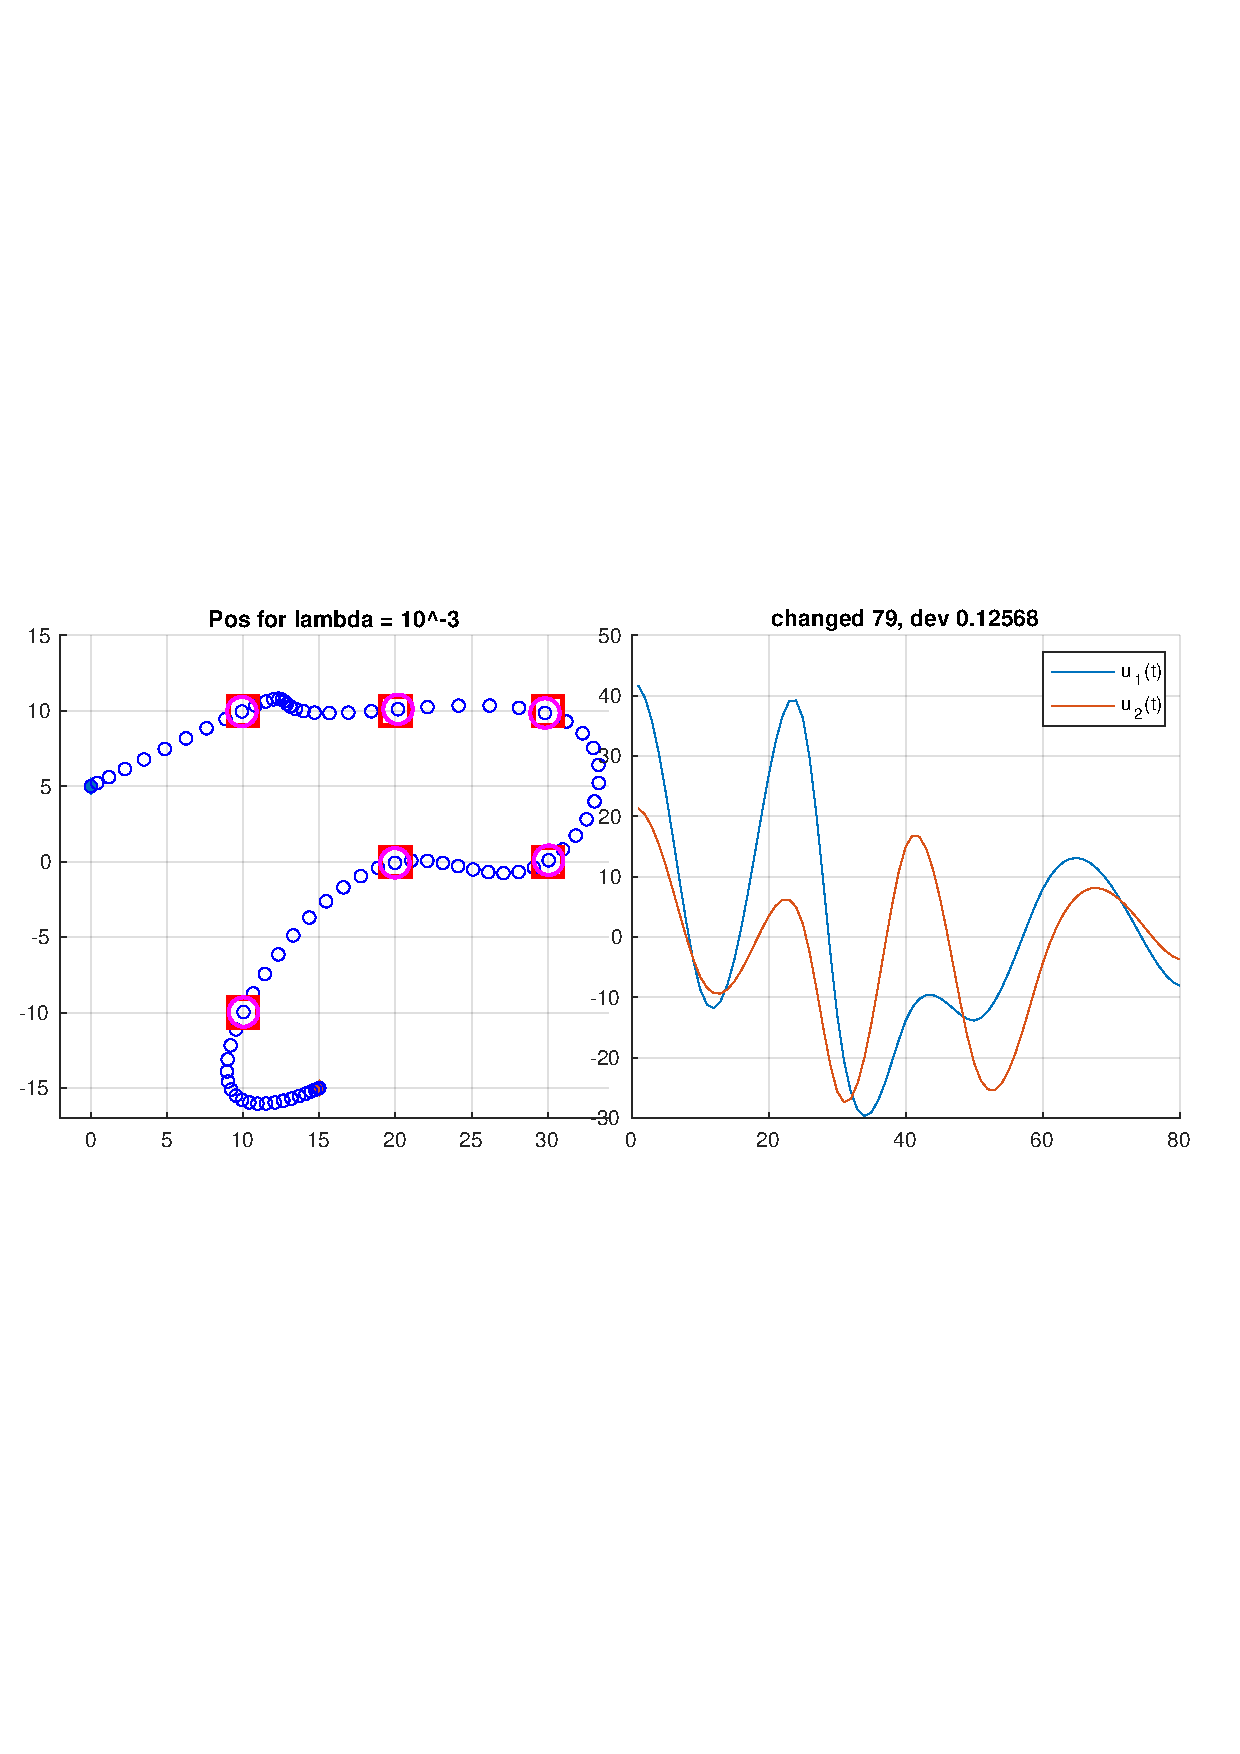
\includegraphics[width=0.5\linewidth]{part1/figures/task1/1_-3.pdf}\hspace{0em}
    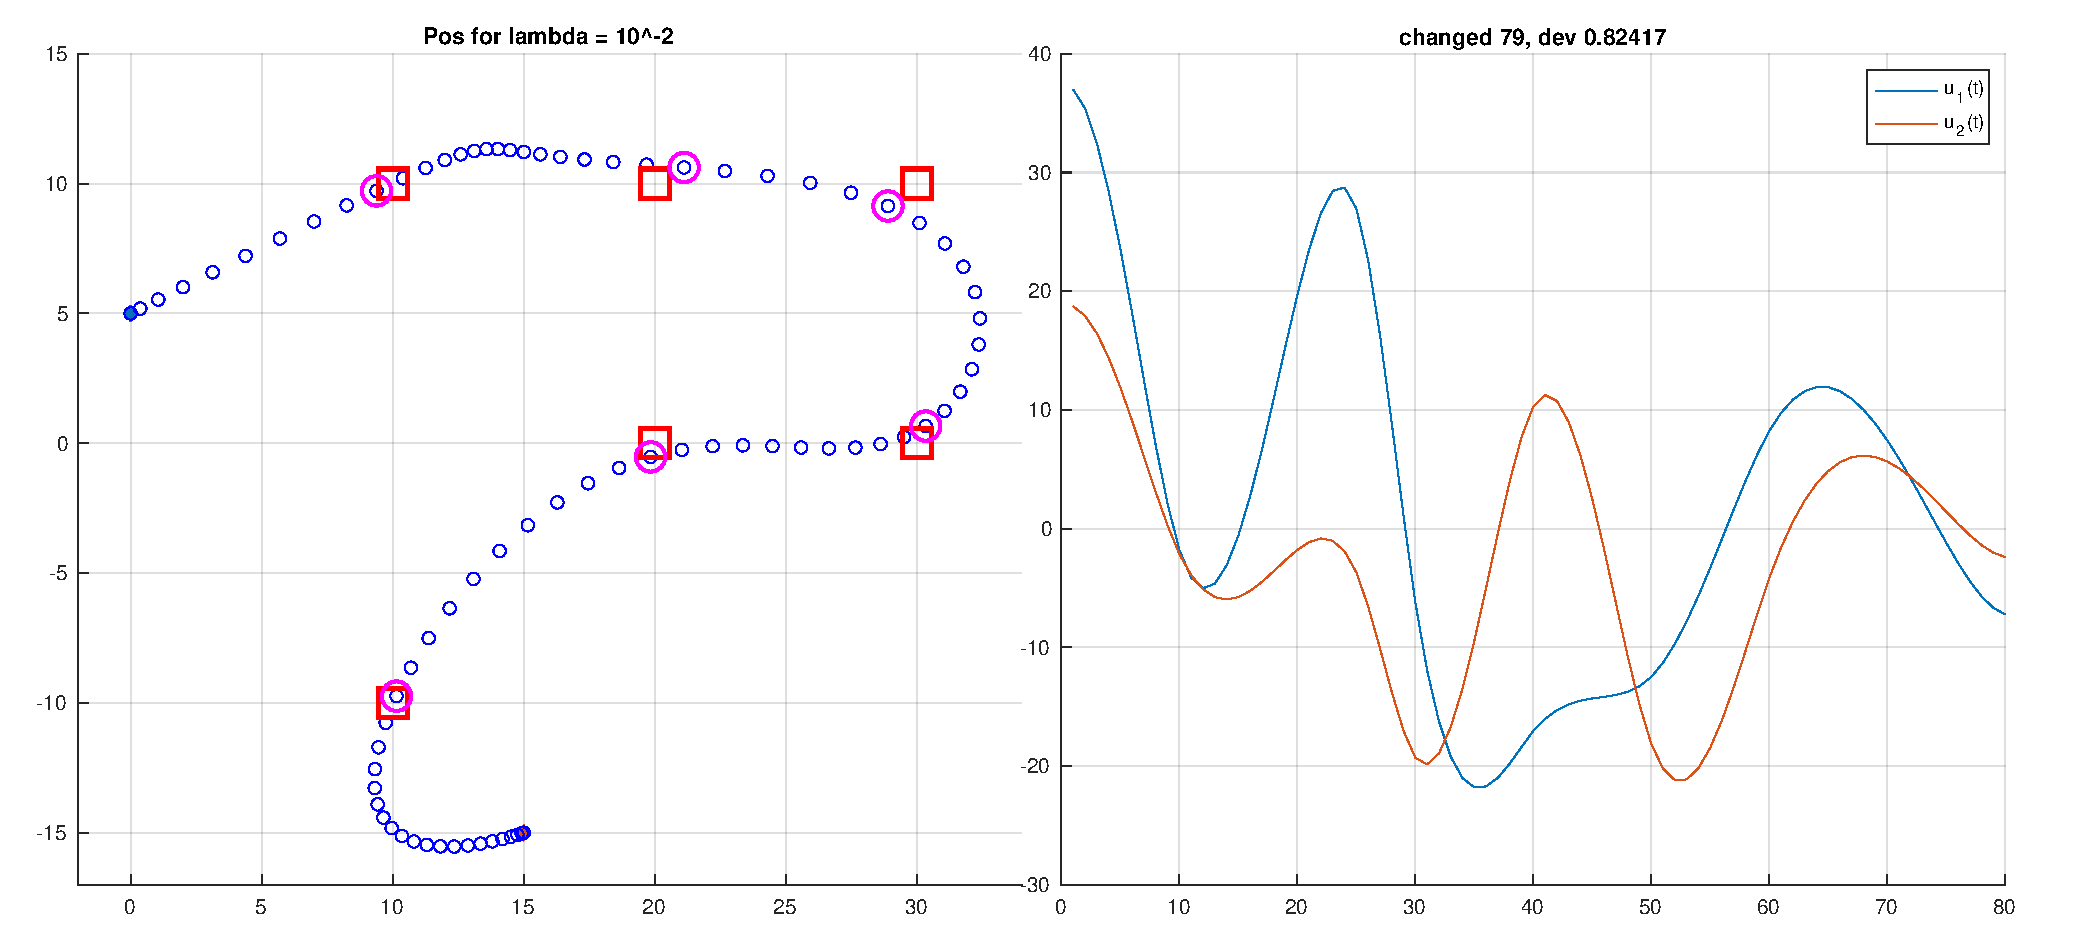
\includegraphics[width=0.5\linewidth]{part1/figures/task1/1_-2.pdf}
\end{subfigure}
\begin{subfigure}
    \centering
    \makebox[\linewidth]{%
        \hspace*{4px}
        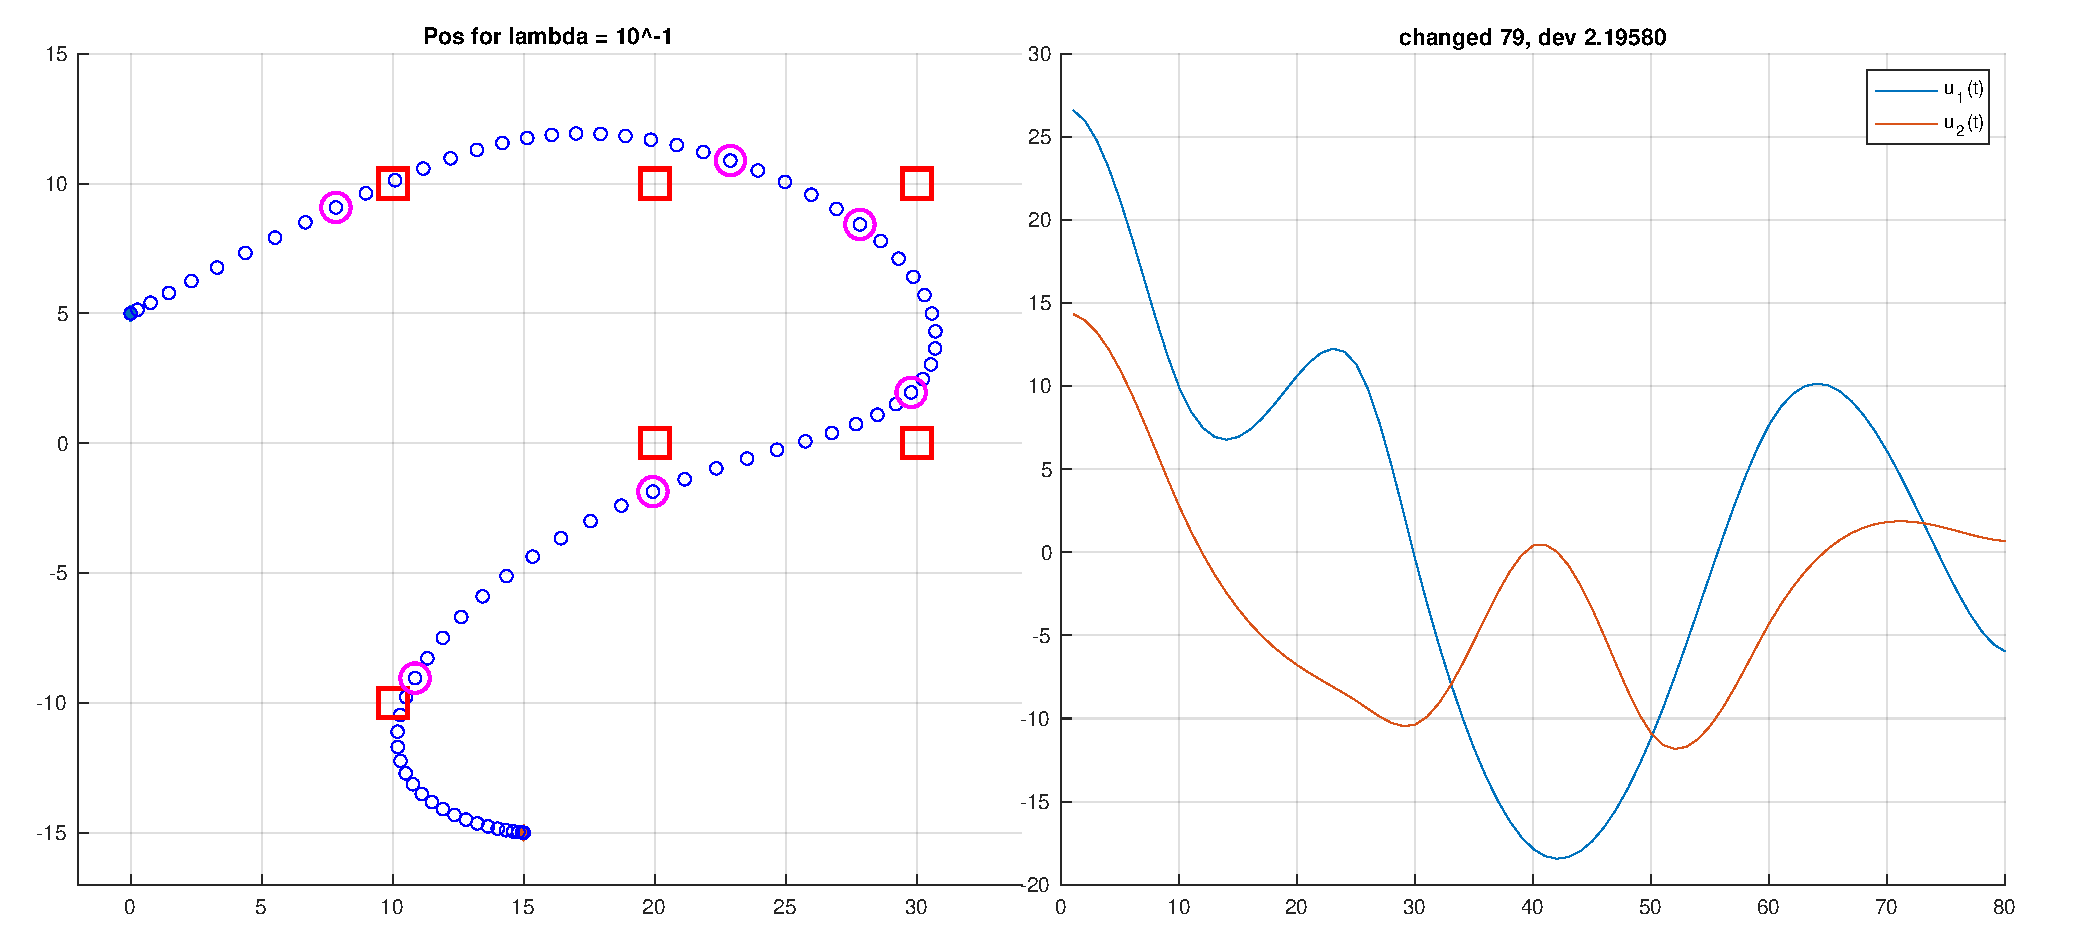
\includegraphics[width=\linewidth + 22px]{part1/figures/task1/1_-1.pdf}
    }
\end{subfigure}
\begin{subfigure}
    \centering
    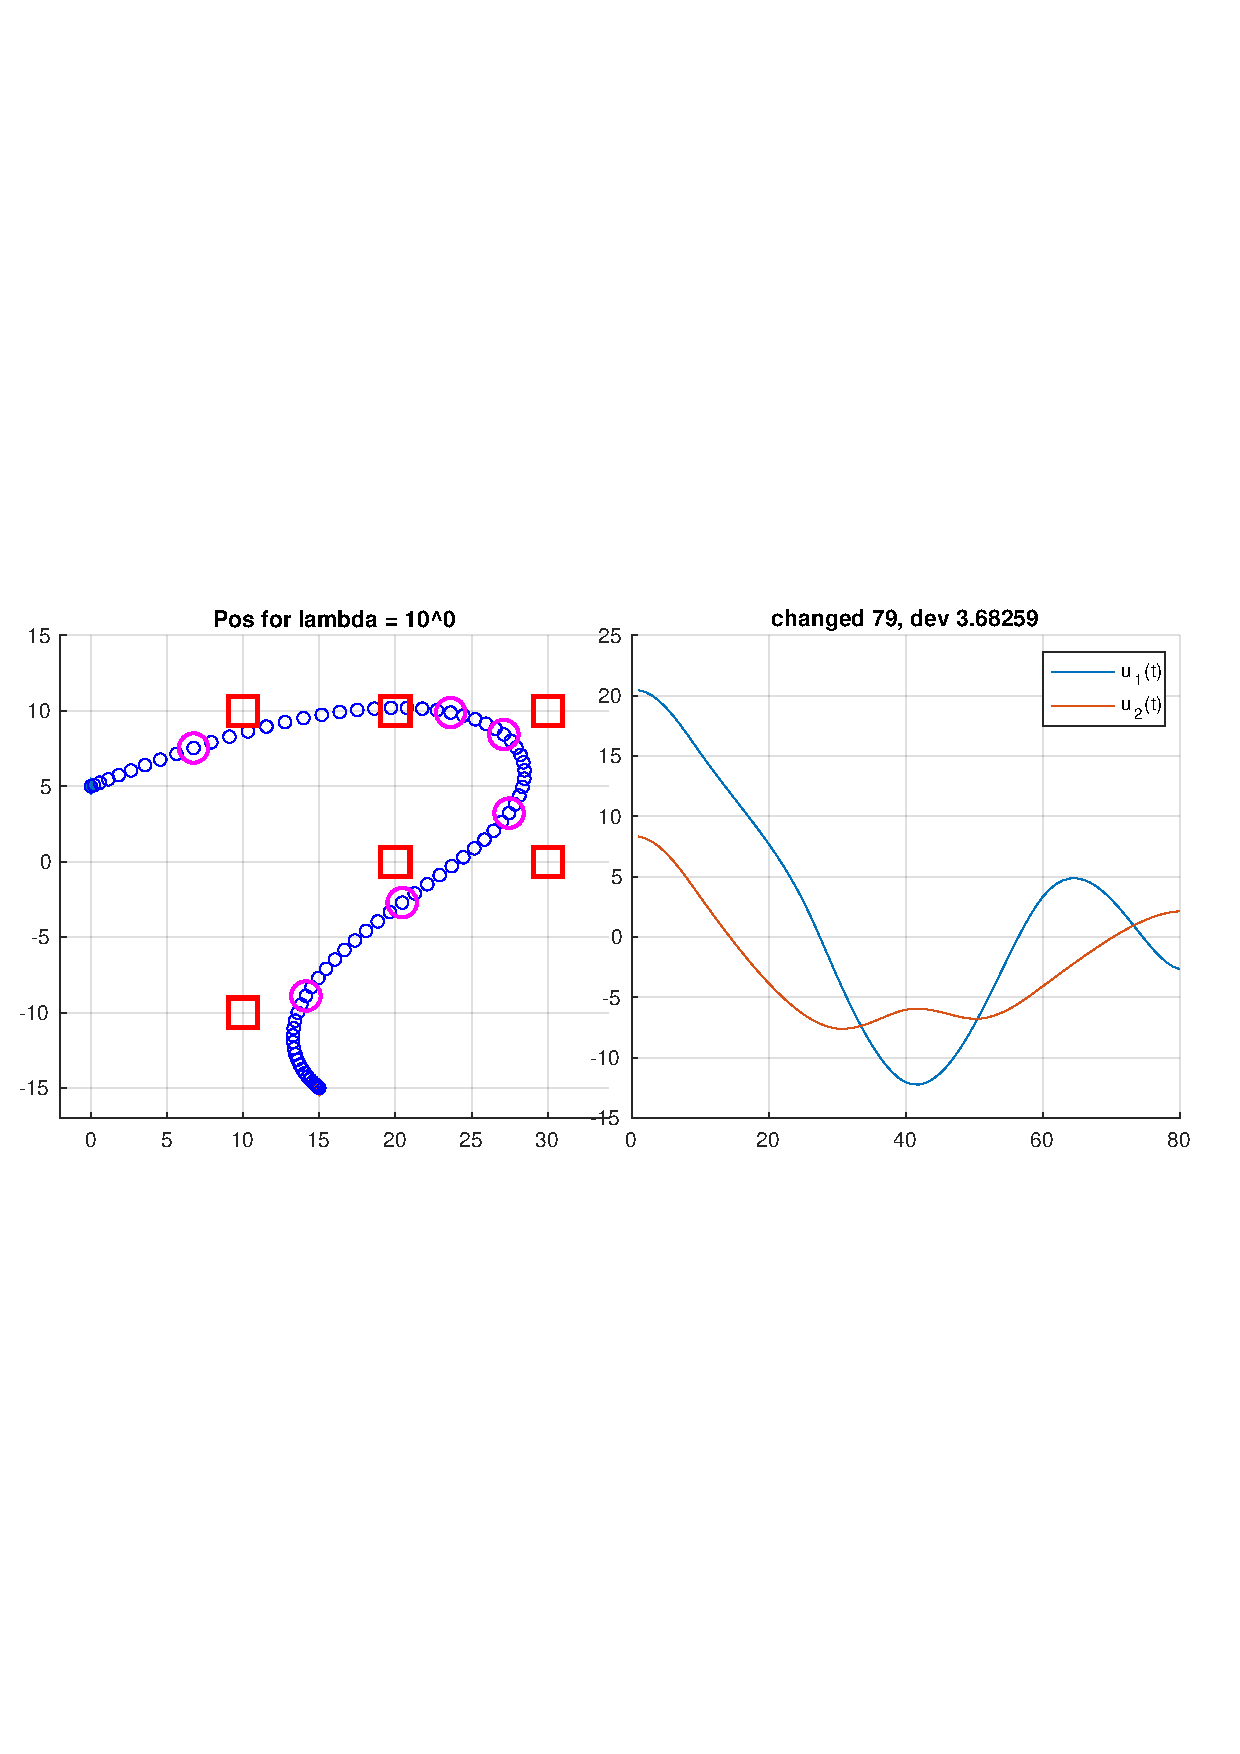
\includegraphics[width=0.5\linewidth]{part1/figures/task1/1_0.pdf}\hspace{0em}
    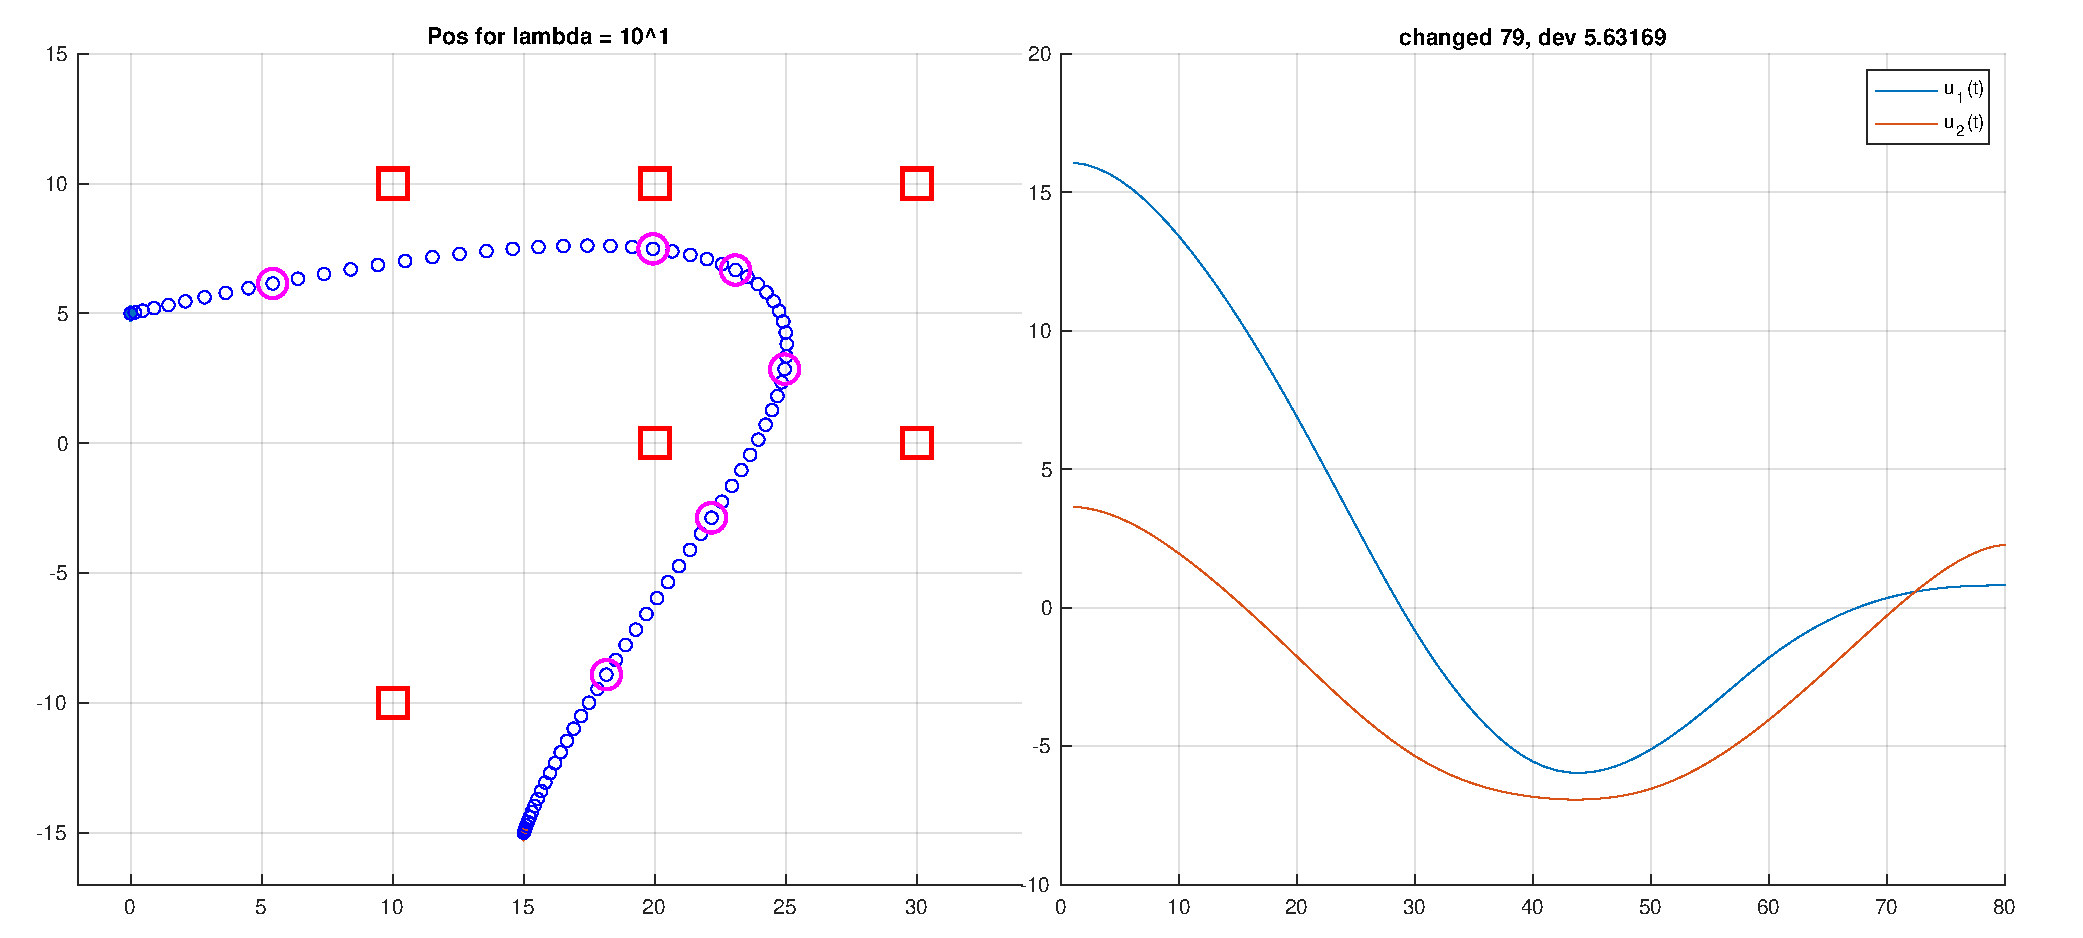
\includegraphics[width=0.5\linewidth]{part1/figures/task1/1_1.pdf}
\end{subfigure}
\begin{subfigure}
    \centering
    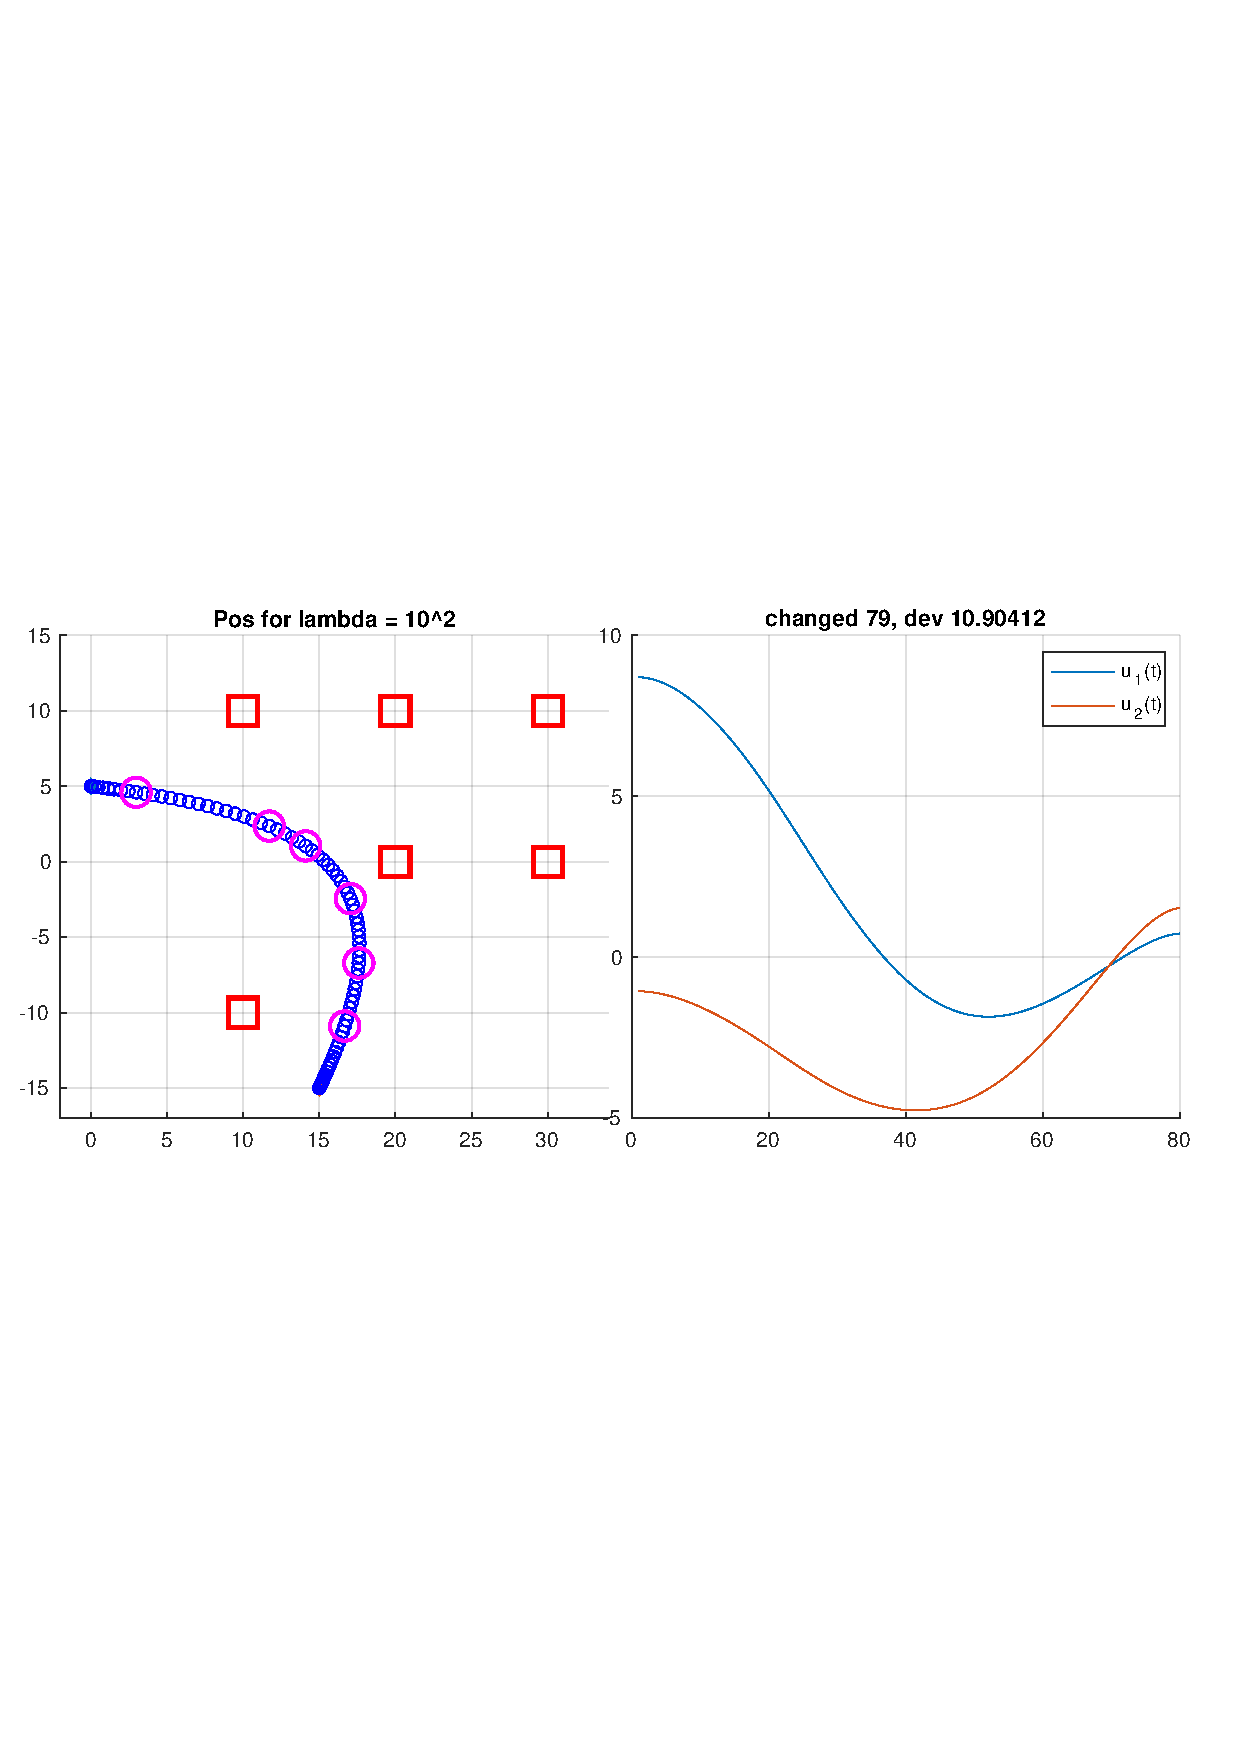
\includegraphics[width=0.5\linewidth]{part1/figures/task1/1_2.pdf}\hspace{0em}
    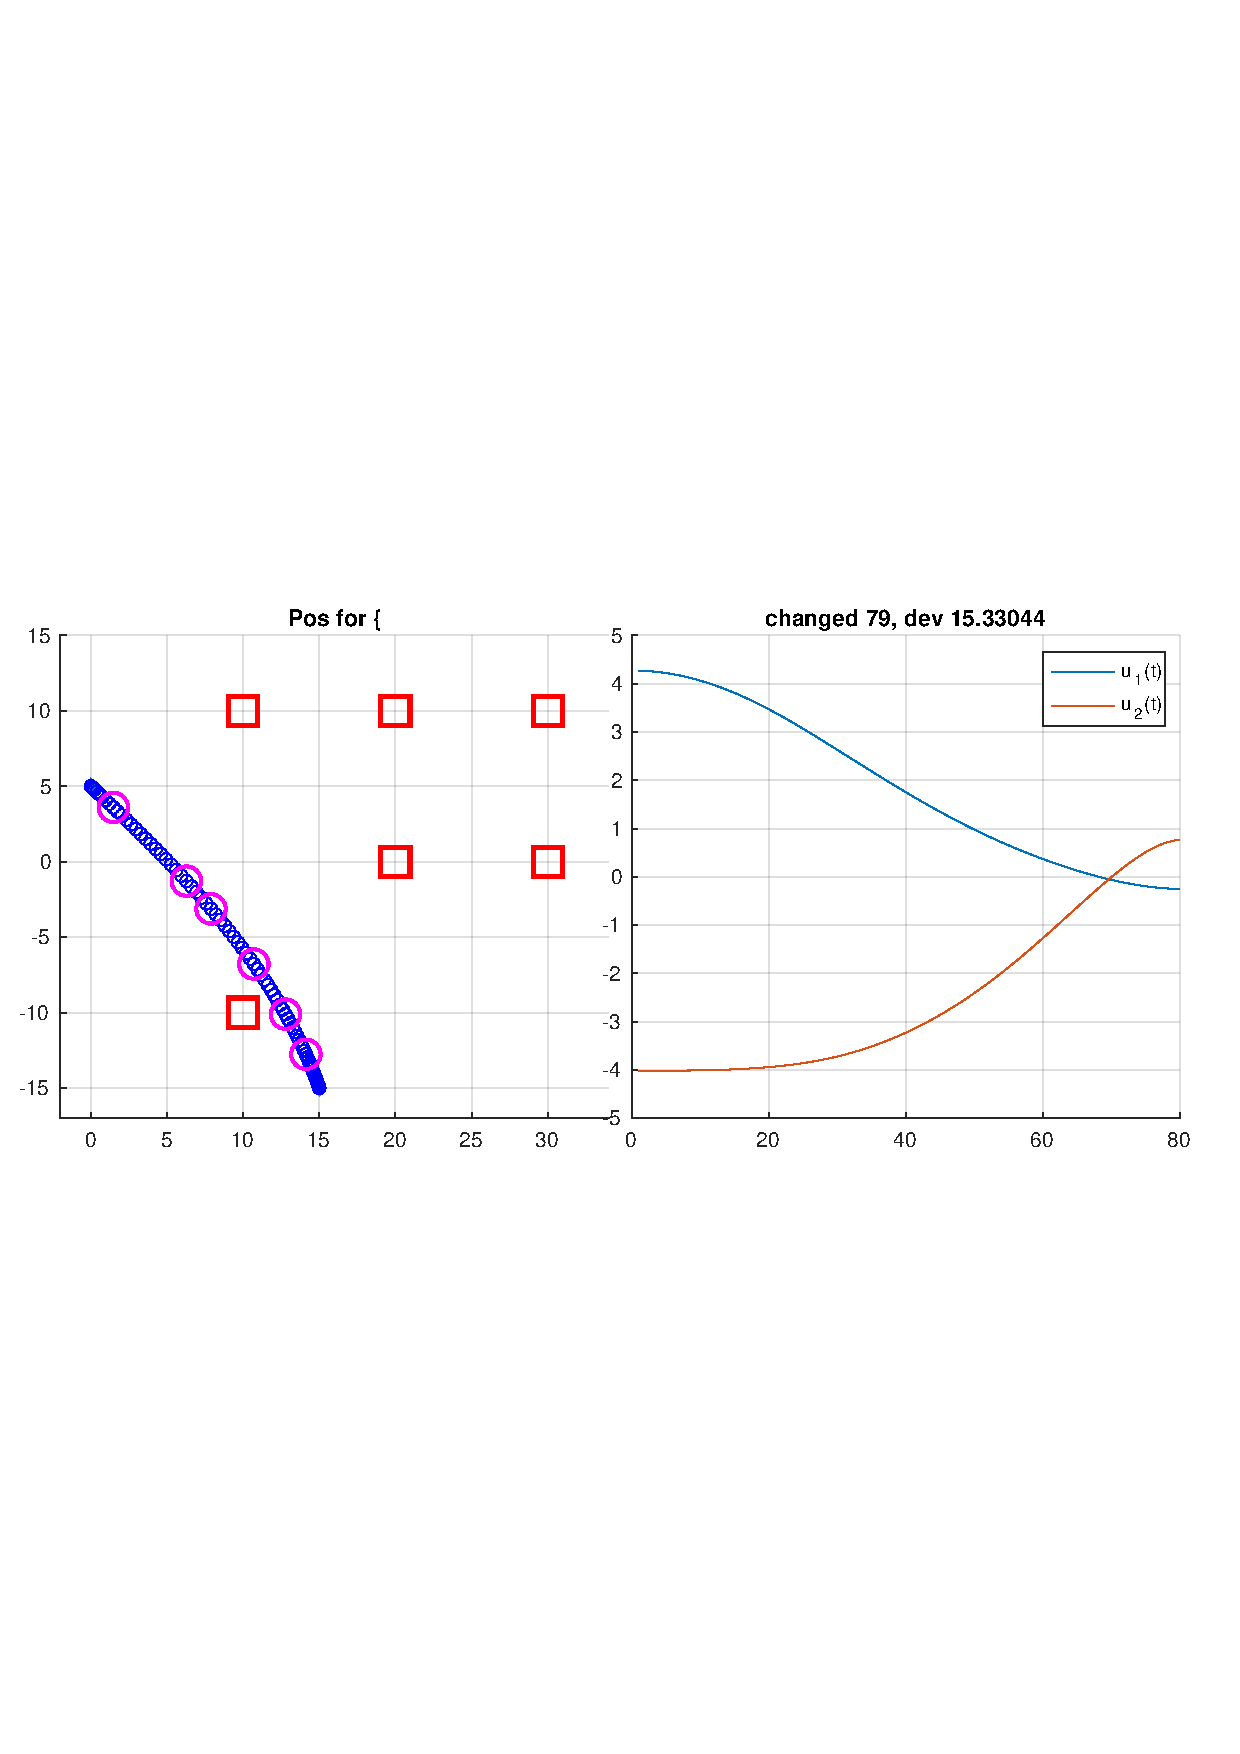
\includegraphics[width=0.5\linewidth]{part1/figures/task1/1_3.pdf}
\end{subfigure}
\end{figure}

\section{Task 2}
%\noindent\fcolorbox{black}{lightgray}{
%    \parbox{\textwidth}{ \textbf{Task 2.} Redo task 1 for the optimization problem~\eqref{prob2}. 
%    }
%}
Code utilized in the task 2 is same as in Task 1, except for the objective function, which is defined as described in Listing \ref{task2:code:objective}. The results are described in the Table \ref{task2:table:results}.

\begin{lstlisting}[label=task2:code:objective, caption=Objective function used in Task 2., float=!htb]
minimize(sum(vec_sqr_sum(E*x(:,tau+1) - w))...
    + lambda*sum(norms(delta, 2)));
\end{lstlisting}

\begin{figure}[!htb]
\caption{Robot positions and control signal for Task 2.}
\label{fig:task2:graphs}
\begin{subfigure}
    \centering
    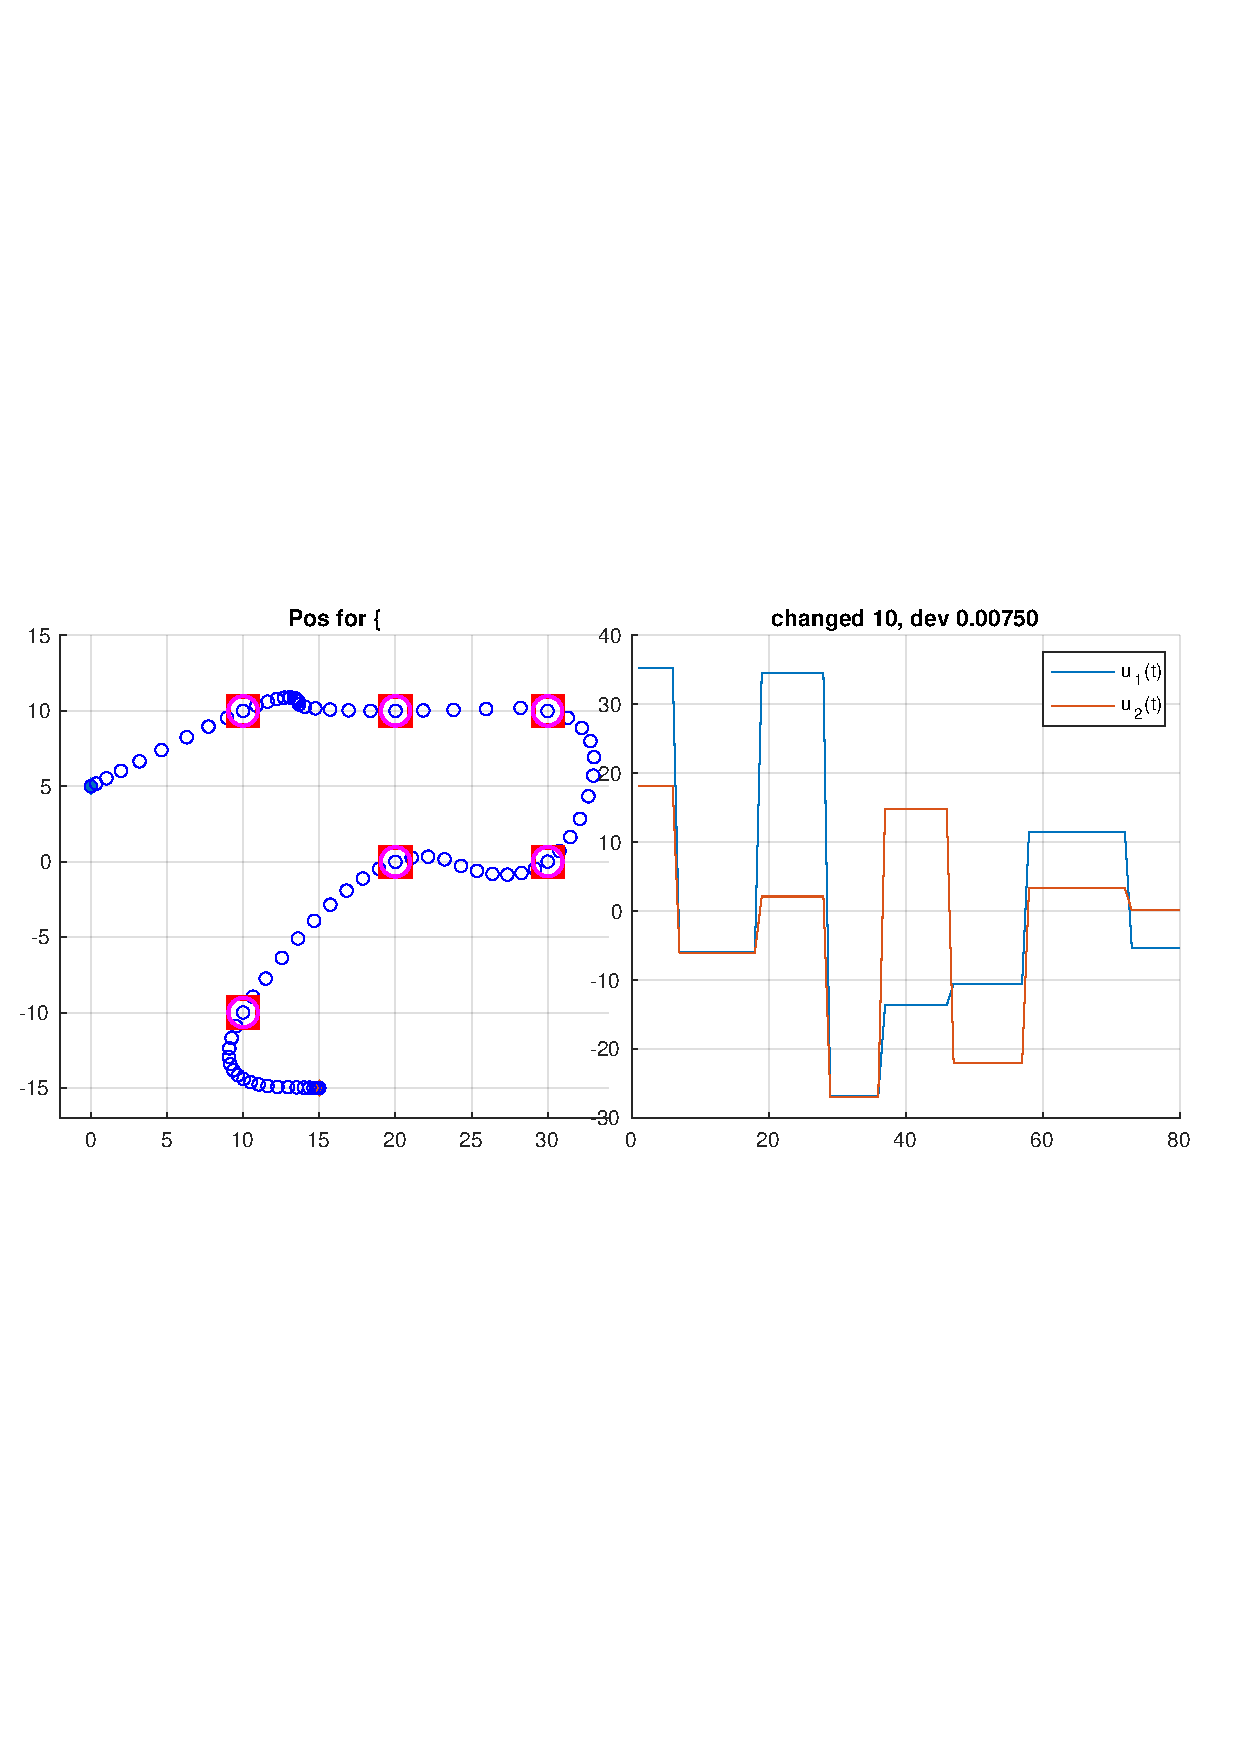
\includegraphics[width=0.5\linewidth]{part1/figures/task2/2_-3.pdf}\hspace{0em}
    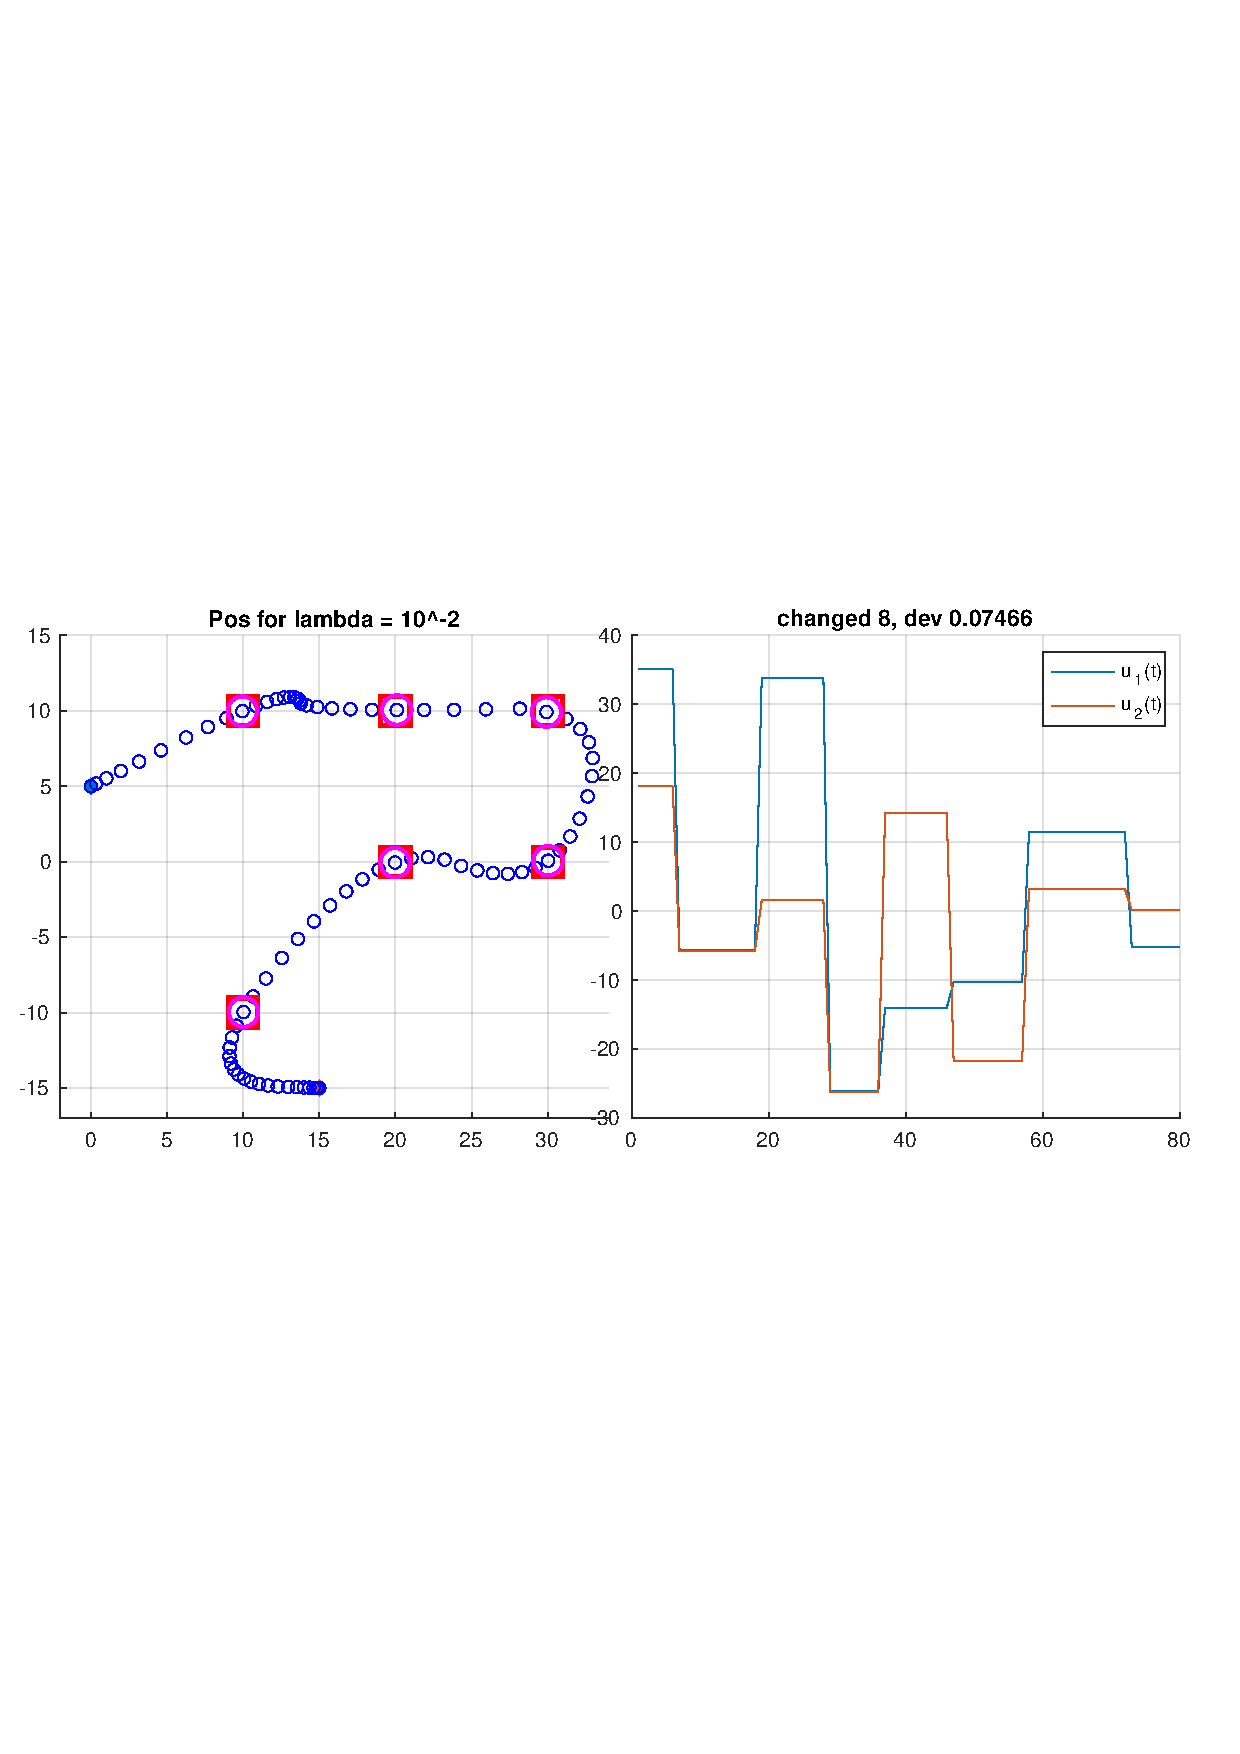
\includegraphics[width=0.5\linewidth]{part1/figures/task2/2_-2.pdf}
\end{subfigure}
\begin{subfigure}
    \centering
    \makebox[\linewidth]{%
        \hspace*{4px}
        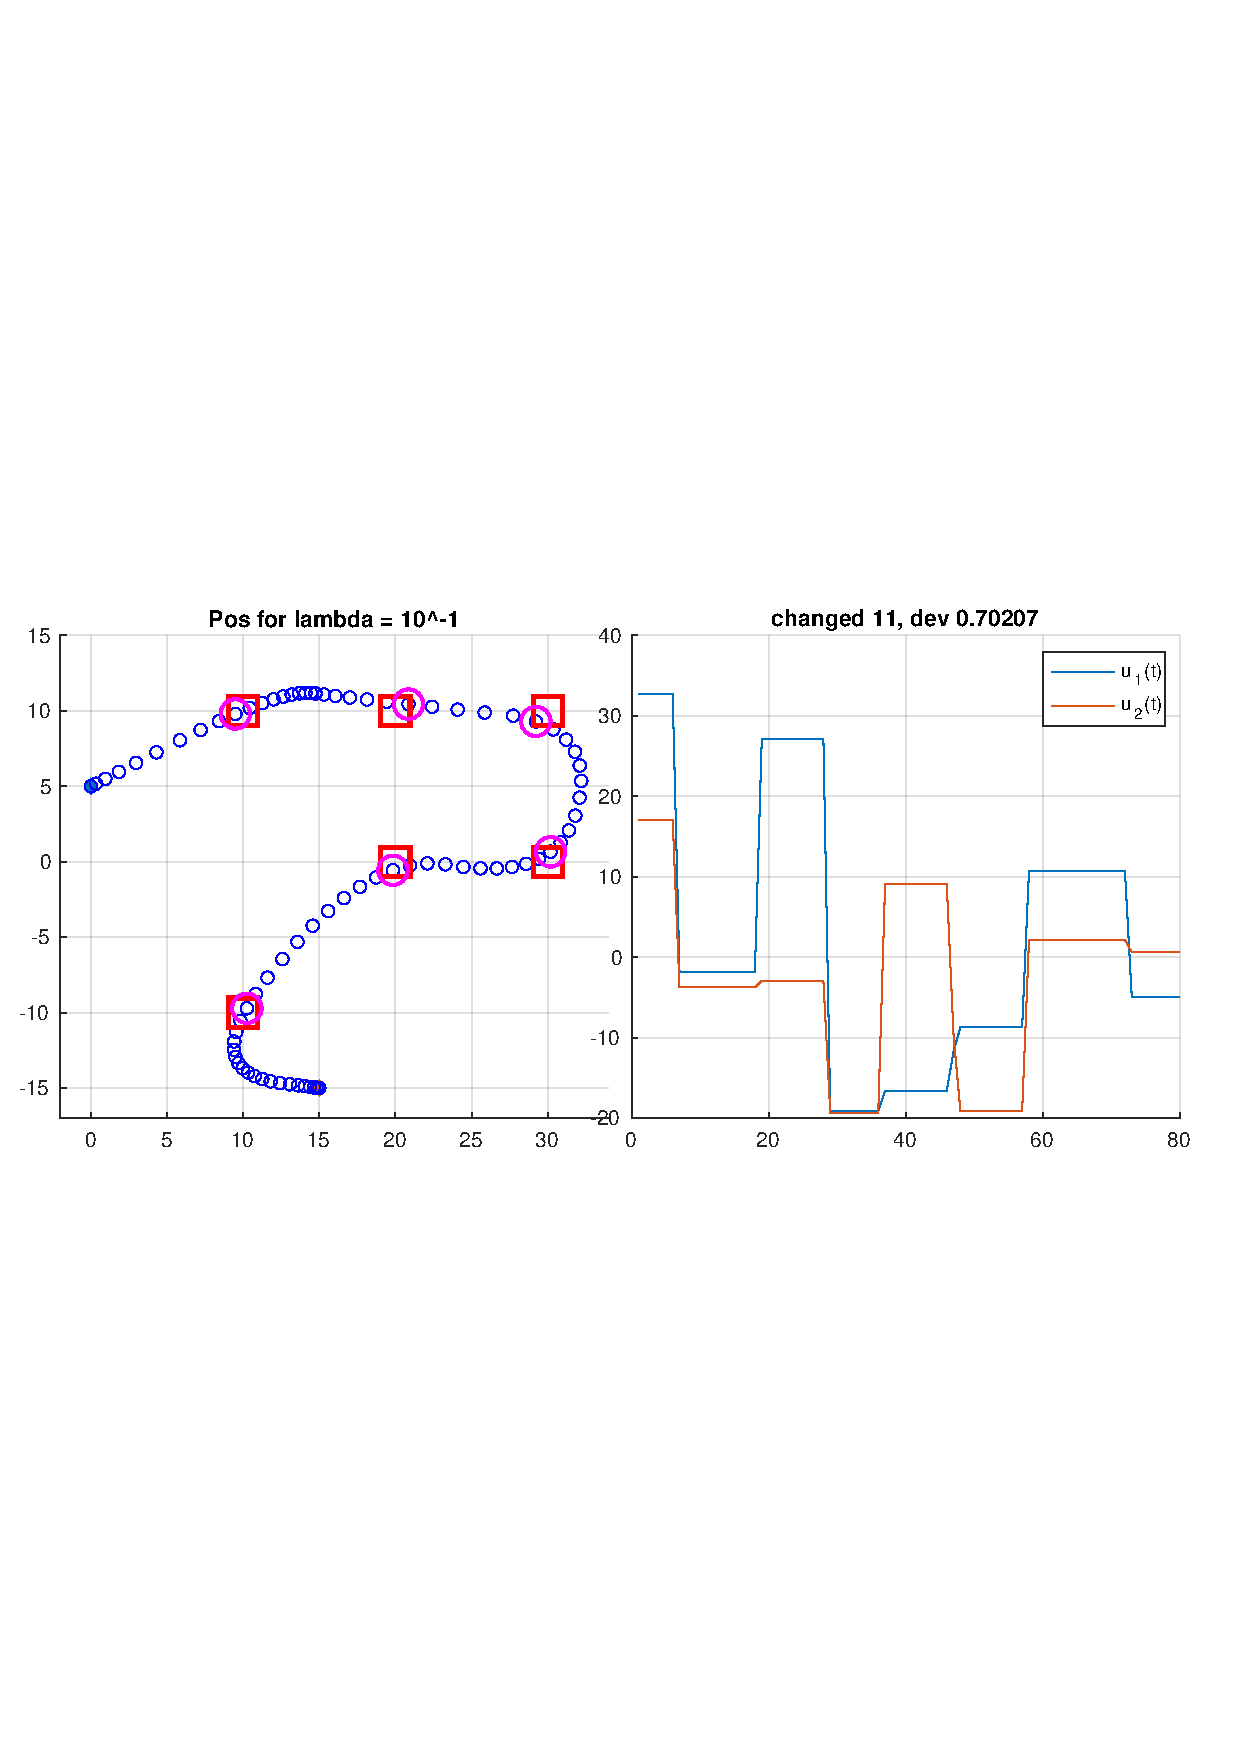
\includegraphics[width=\linewidth + 22px]{part1/figures/task2/2_-1.pdf}
    }
\end{subfigure}
\begin{subfigure}
    \centering
    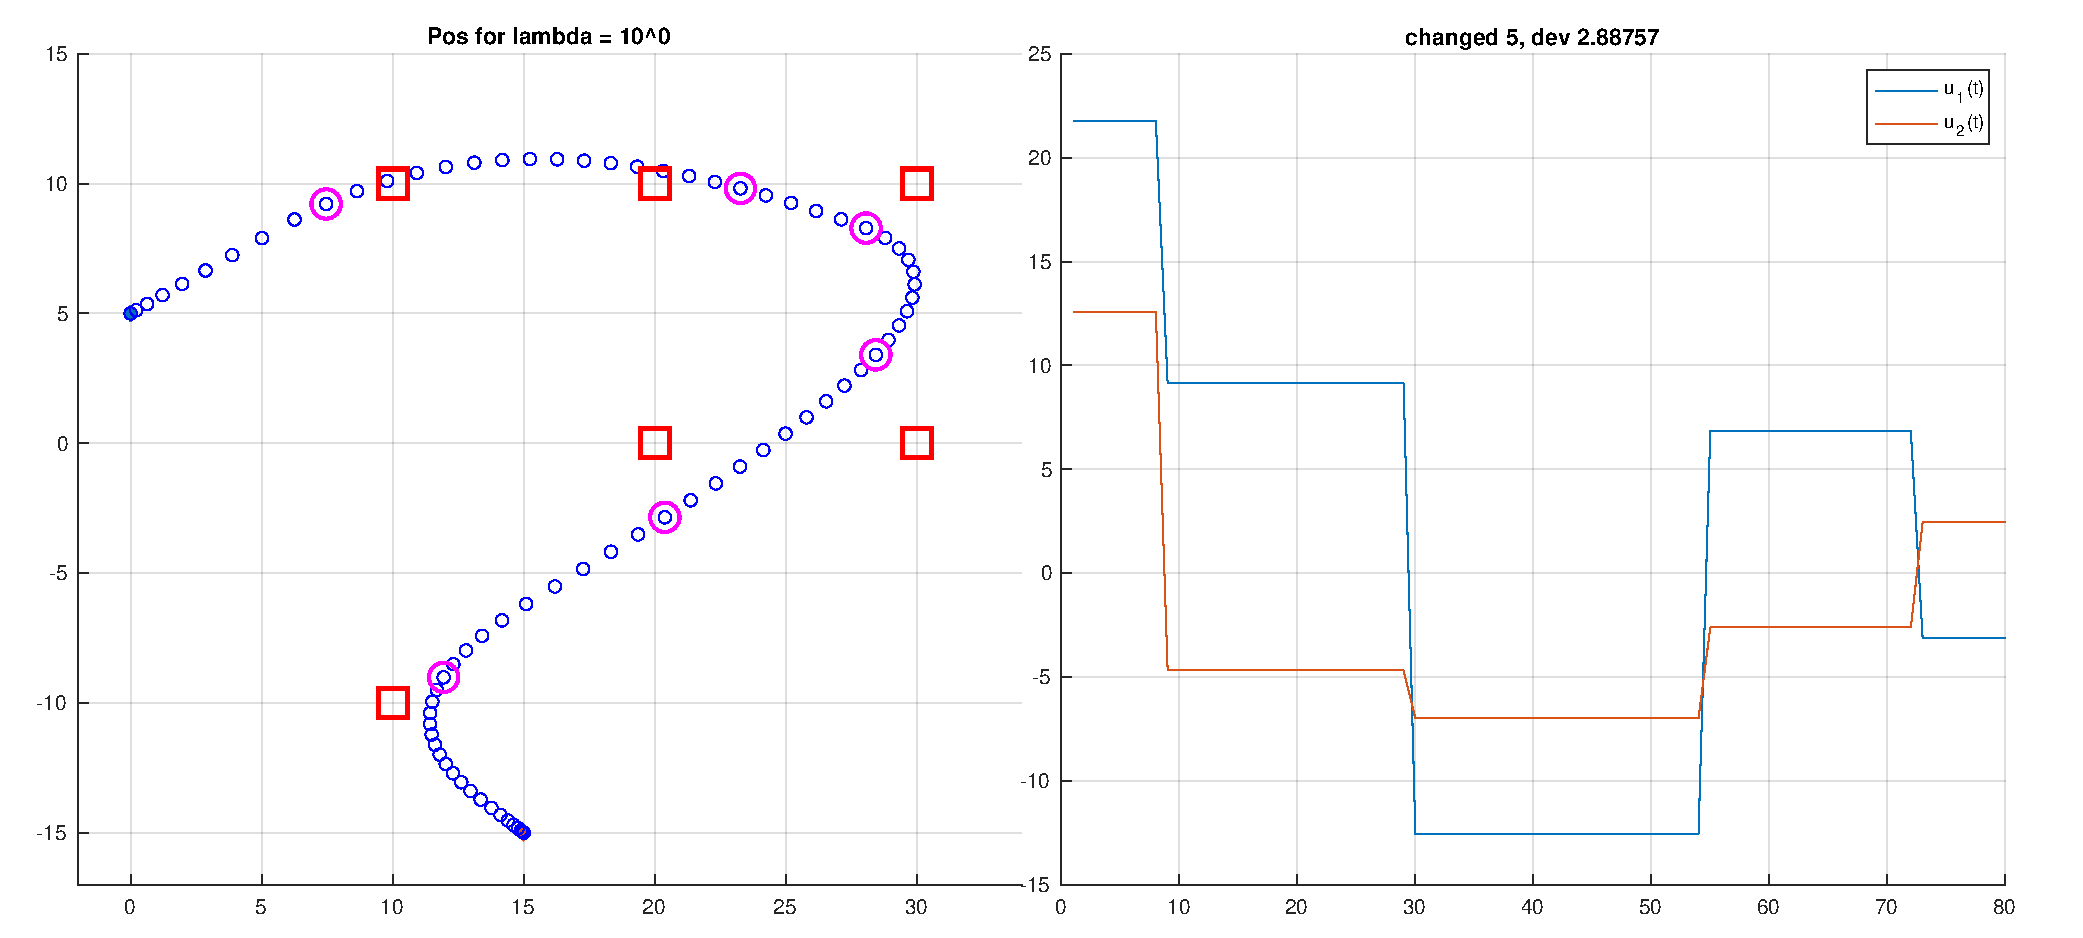
\includegraphics[width=0.5\linewidth]{part1/figures/task2/2_0.pdf}\hspace{0em}
    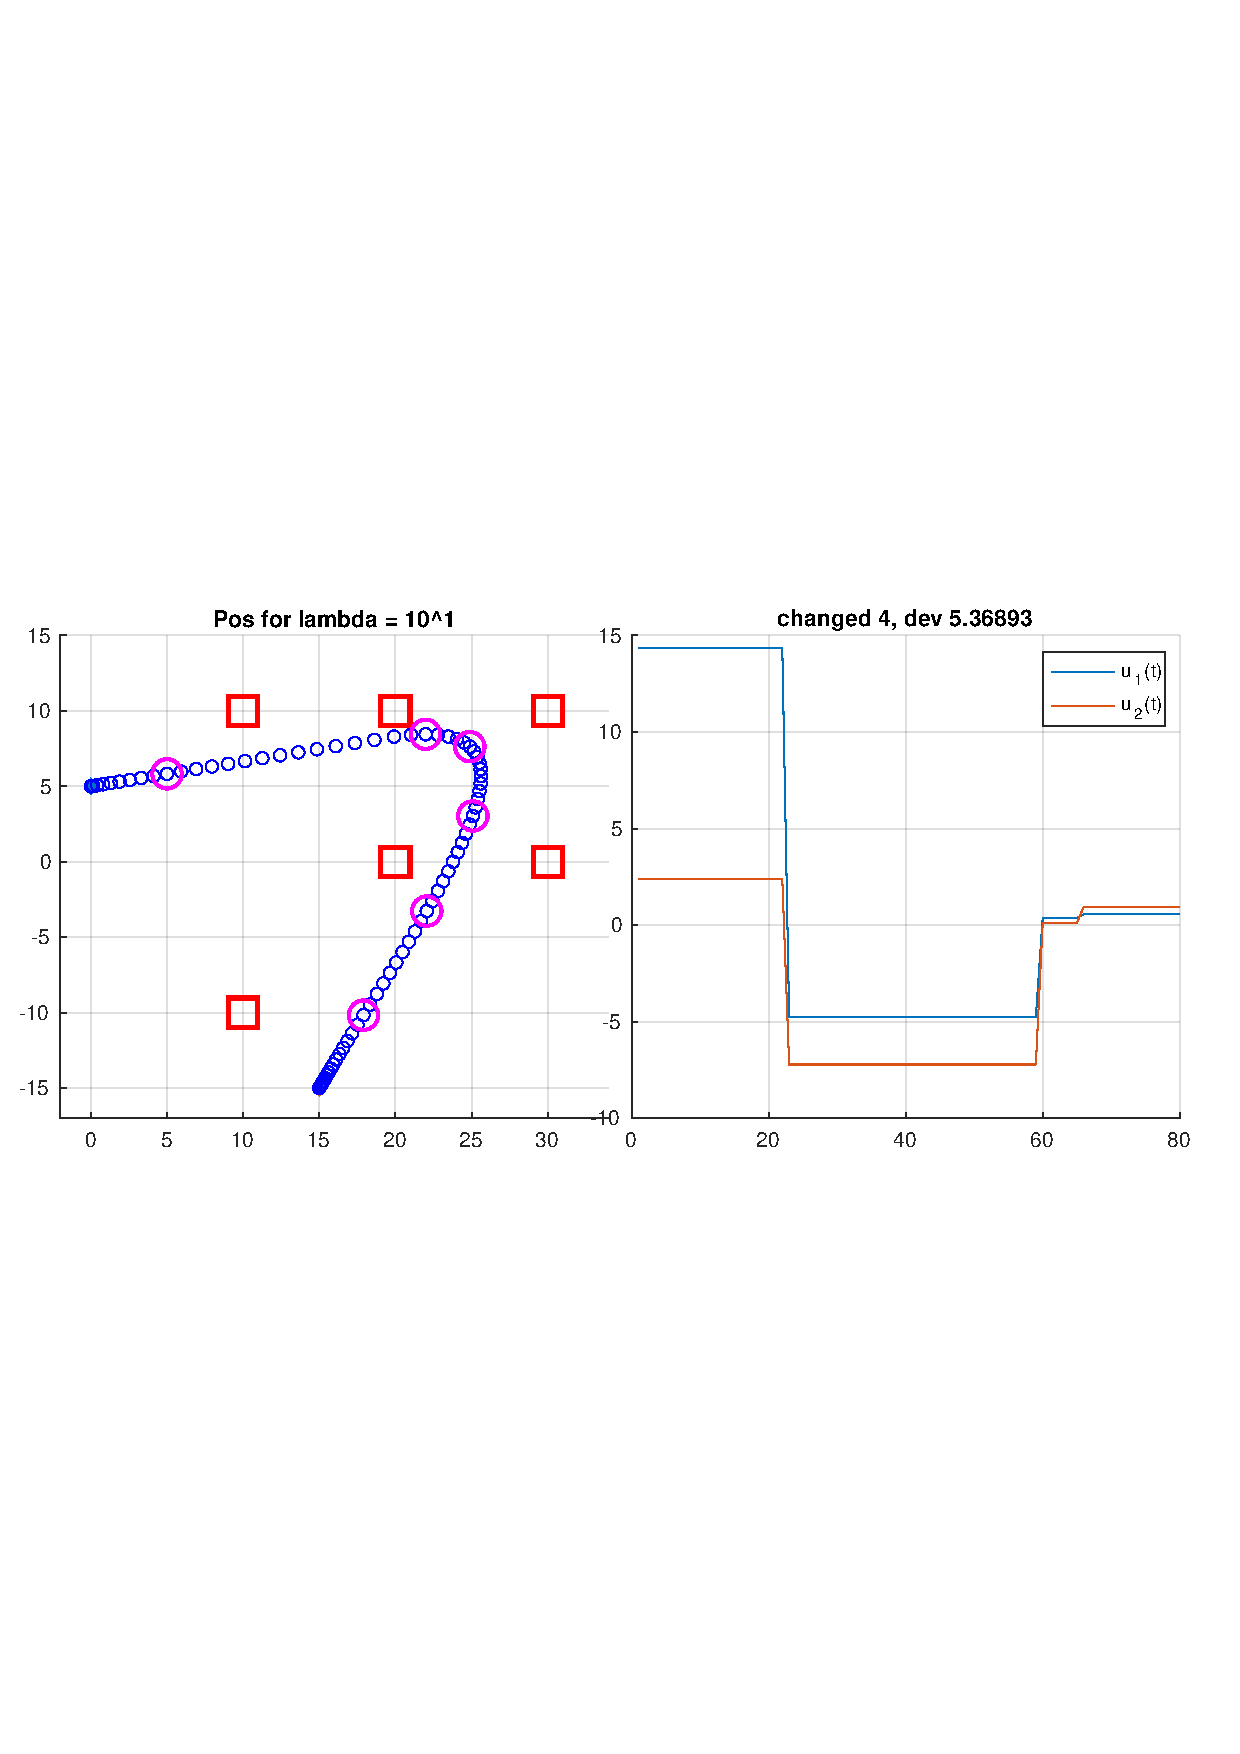
\includegraphics[width=0.5\linewidth]{part1/figures/task2/2_1.pdf}
\end{subfigure}
\begin{subfigure}
    \centering
    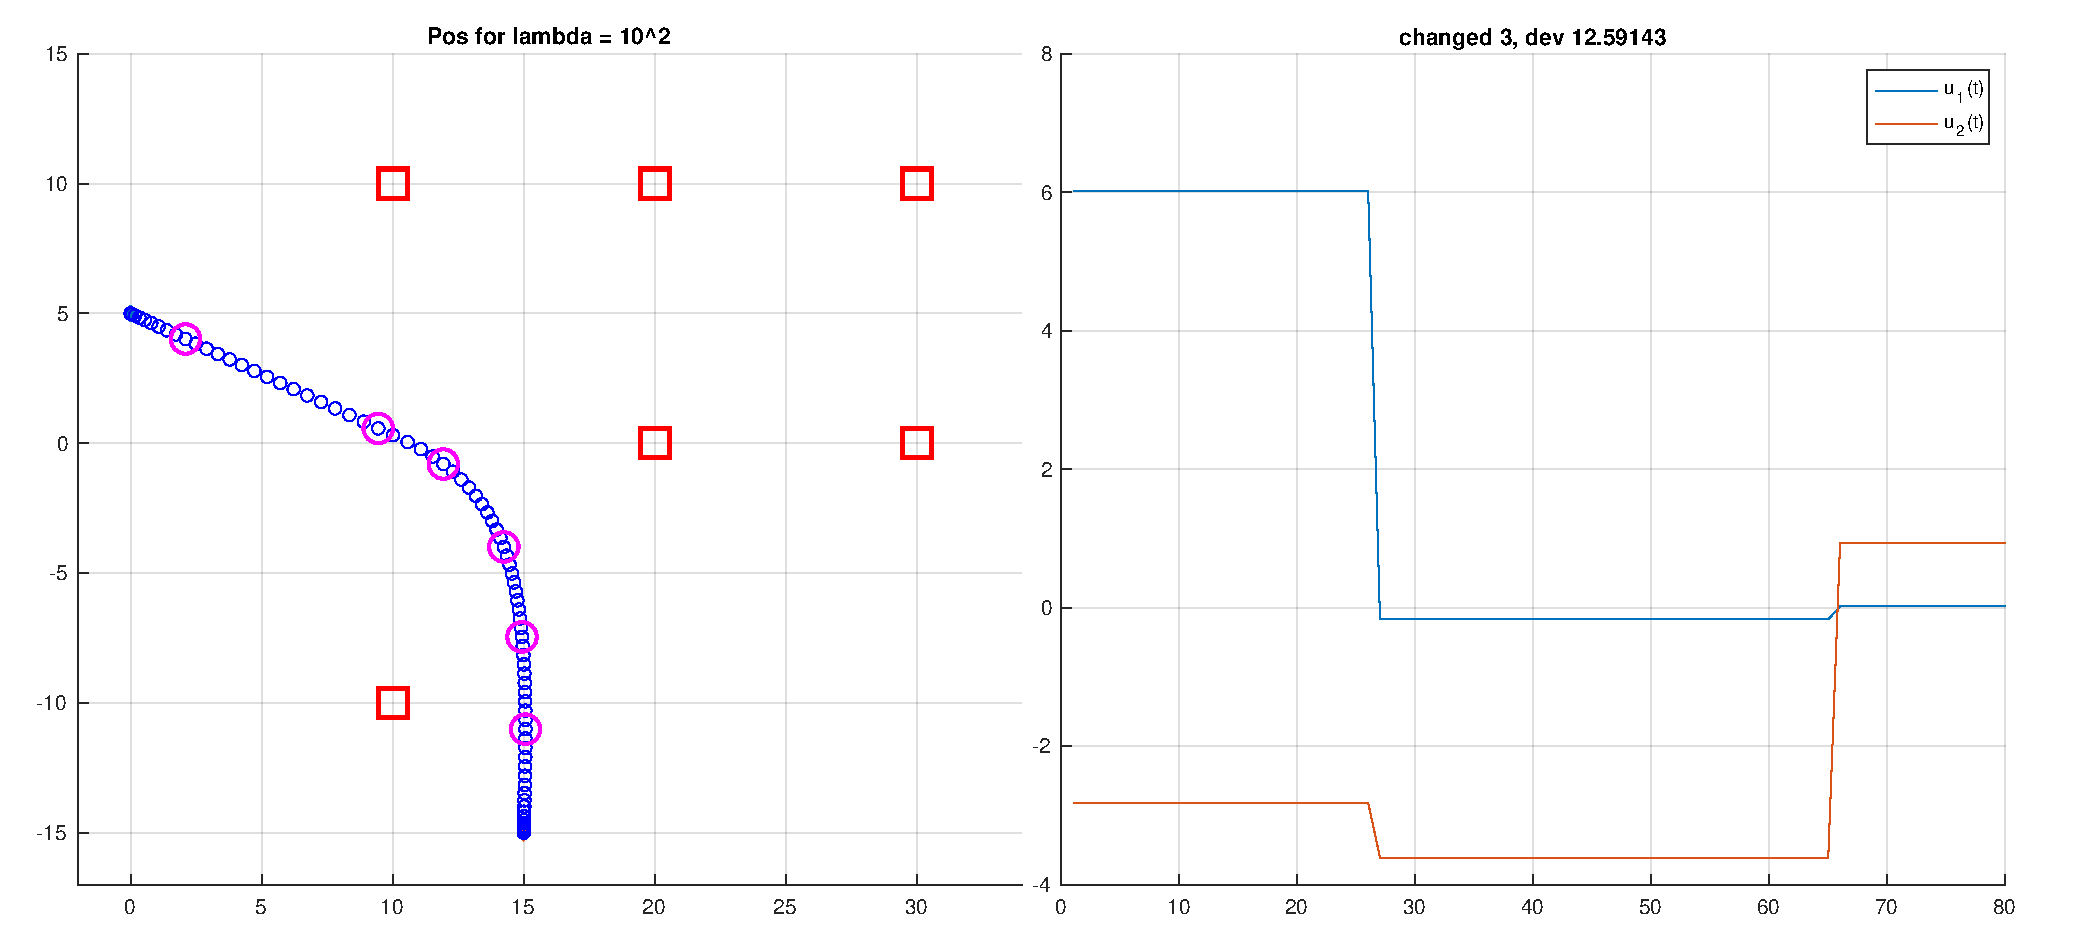
\includegraphics[width=0.5\linewidth]{part1/figures/task2/2_2.pdf}\hspace{0em}
    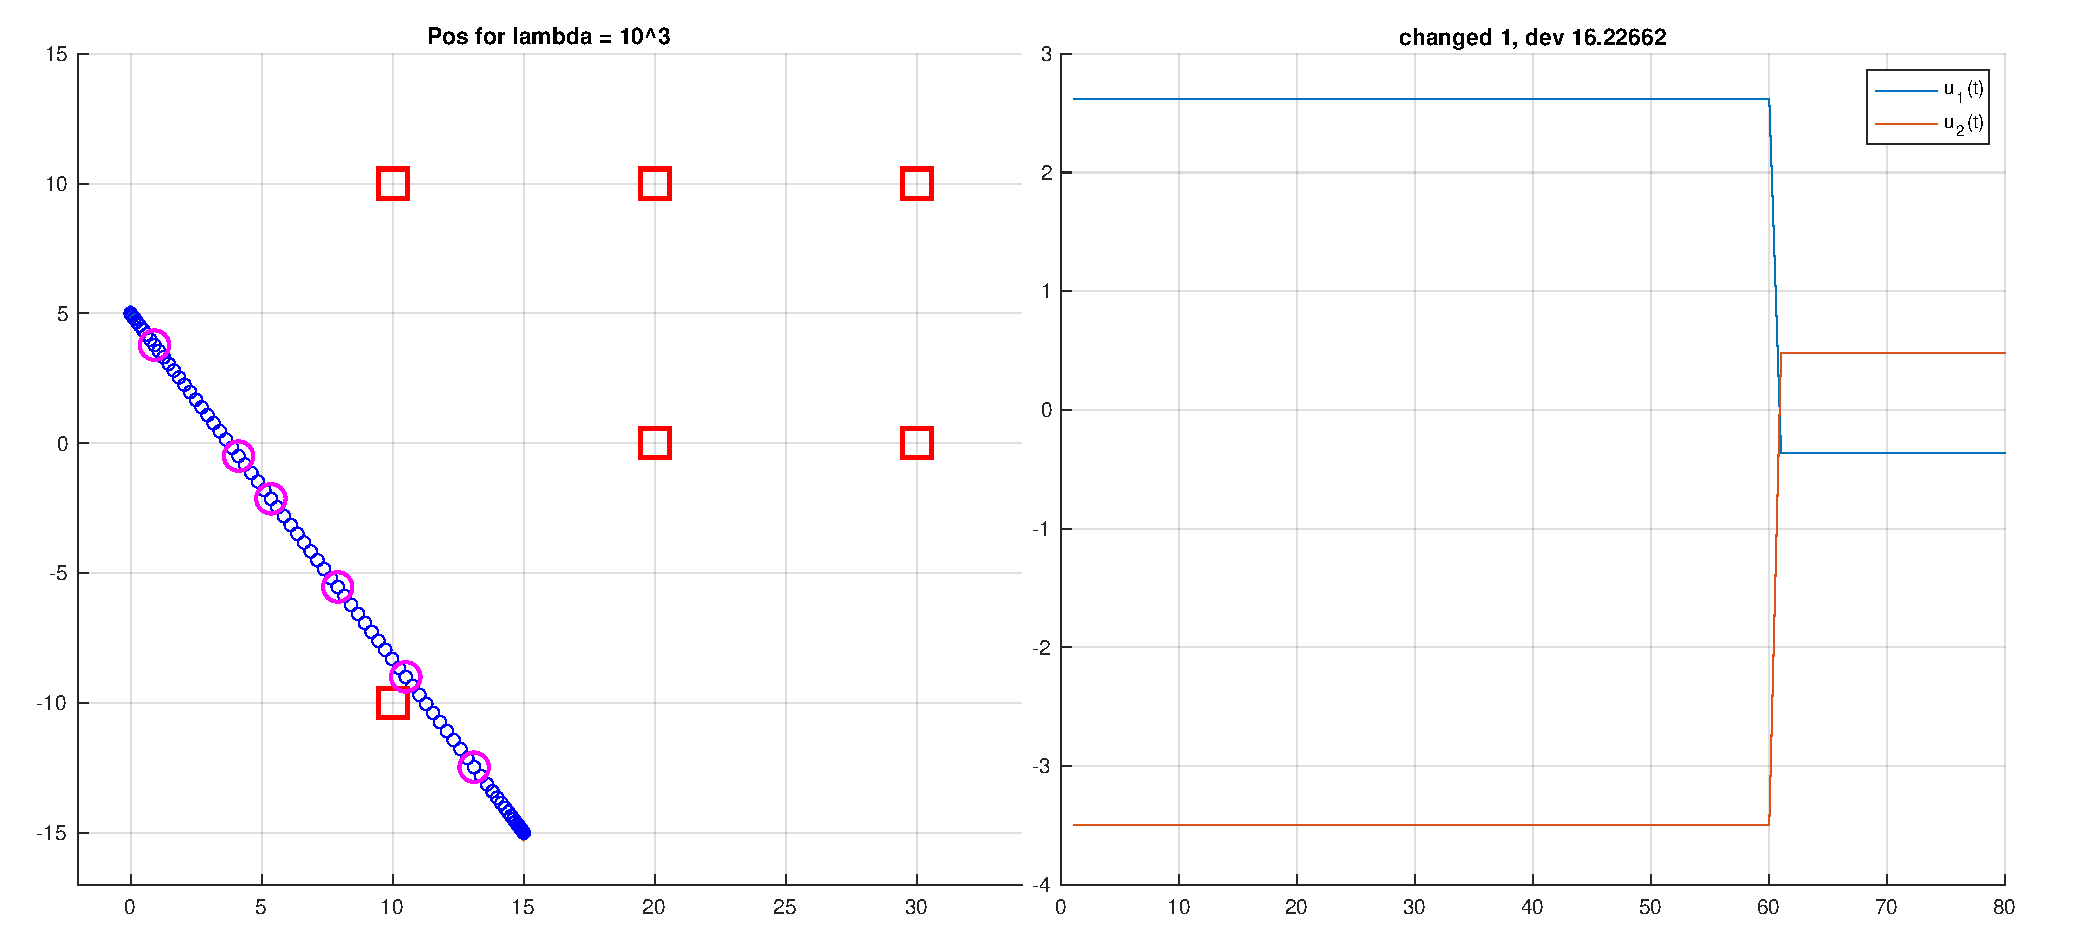
\includegraphics[width=0.5\linewidth]{part1/figures/task2/2_3.pdf}
\end{subfigure}
\end{figure}

\section{Task 3}
%\noindent\fcolorbox{black}{lightgray}{
%    \parbox{\textwidth}{ \textbf{Task 3.} Redo task 1 for the optimization problem~\eqref{prob3}. 
% }}

\begin{lstlisting}[caption=Objective function used in Task 3., label=task3:code:objective, float=!htb]
minimize(sum(vec_sqr_sum(E*x(:,tau+1) - w)...
                ) + lambda*sum(norms(delta, 1)));
\end{lstlisting}

Code utilized in the task 3 is same as in Task 1, except for the objective function, which is defined as described in Listing \ref{task3:code:objective}. The results are described in the Table \ref{task3:table:results}.

\begin{figure}[!htb]
\caption{Robot positions and control signal for Task 3.}
\label{fig:task3:graphs}
\begin{subfigure}
    \centering
    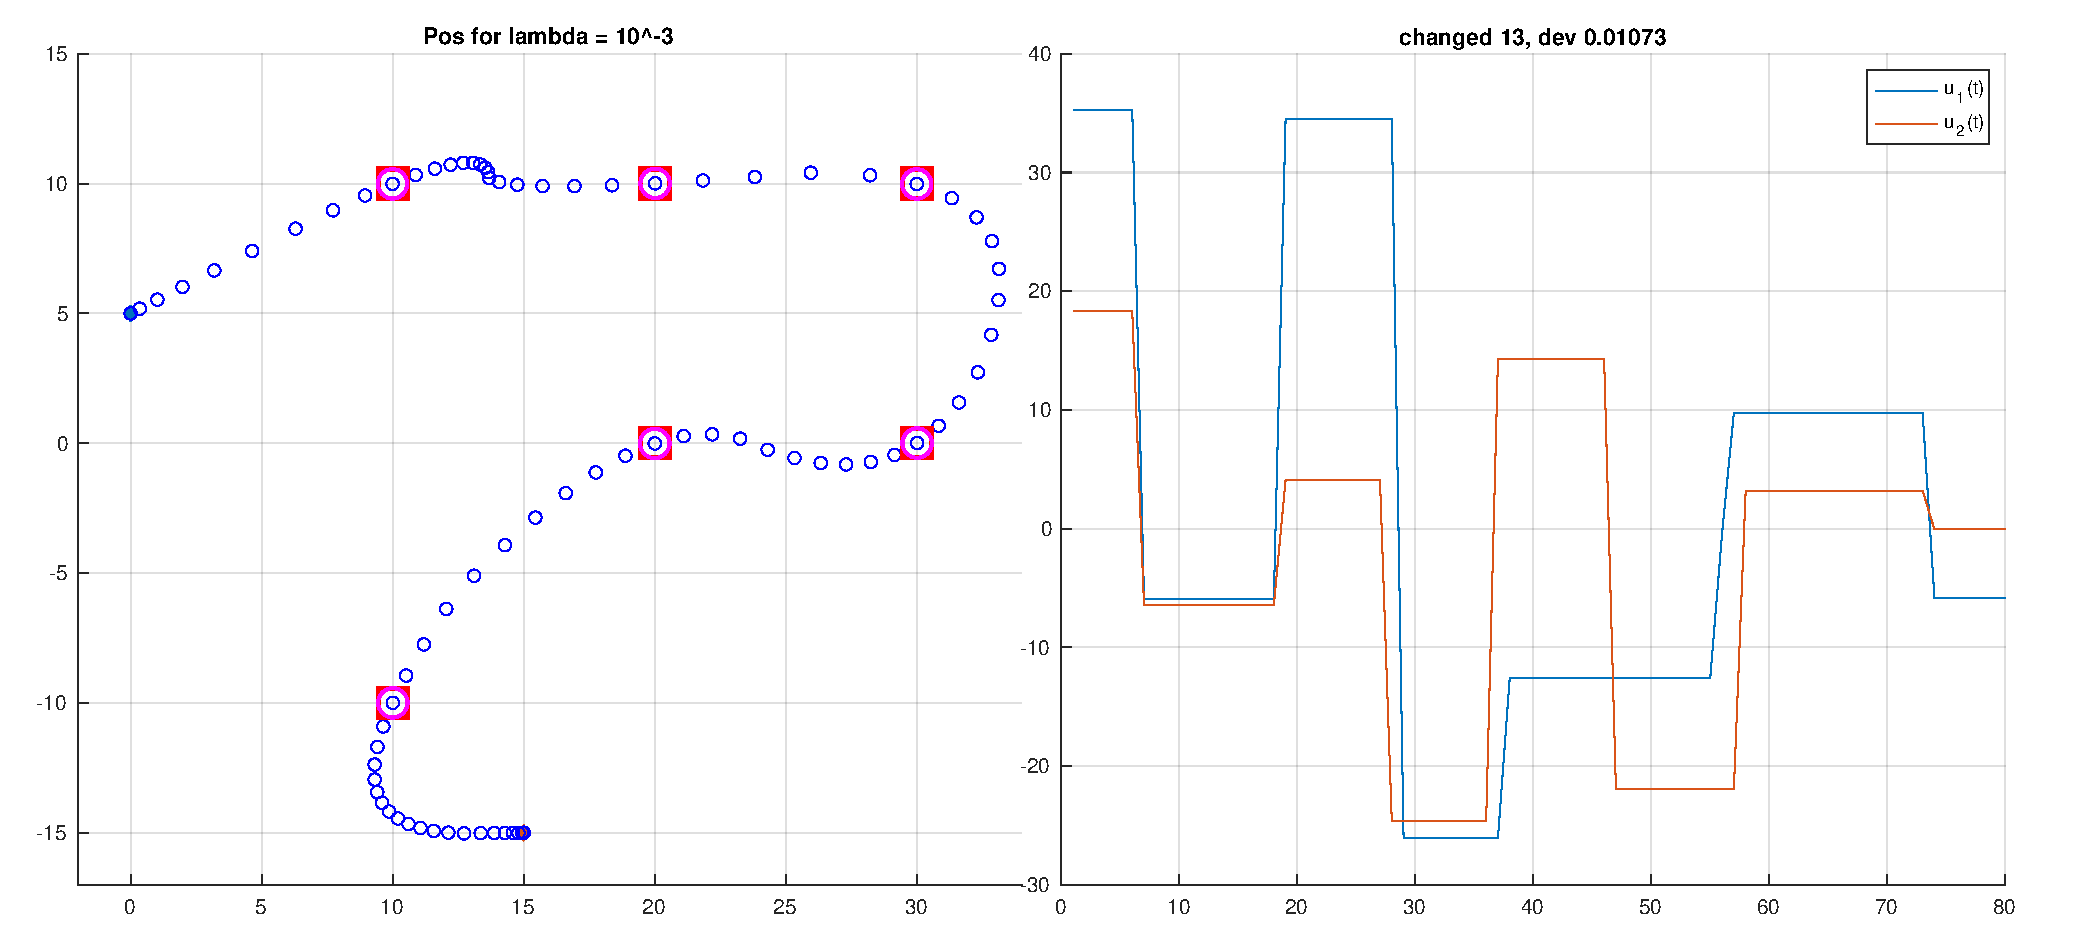
\includegraphics[width=0.5\linewidth]{part1/figures/task3/3_-3.pdf}\hspace{0em}
    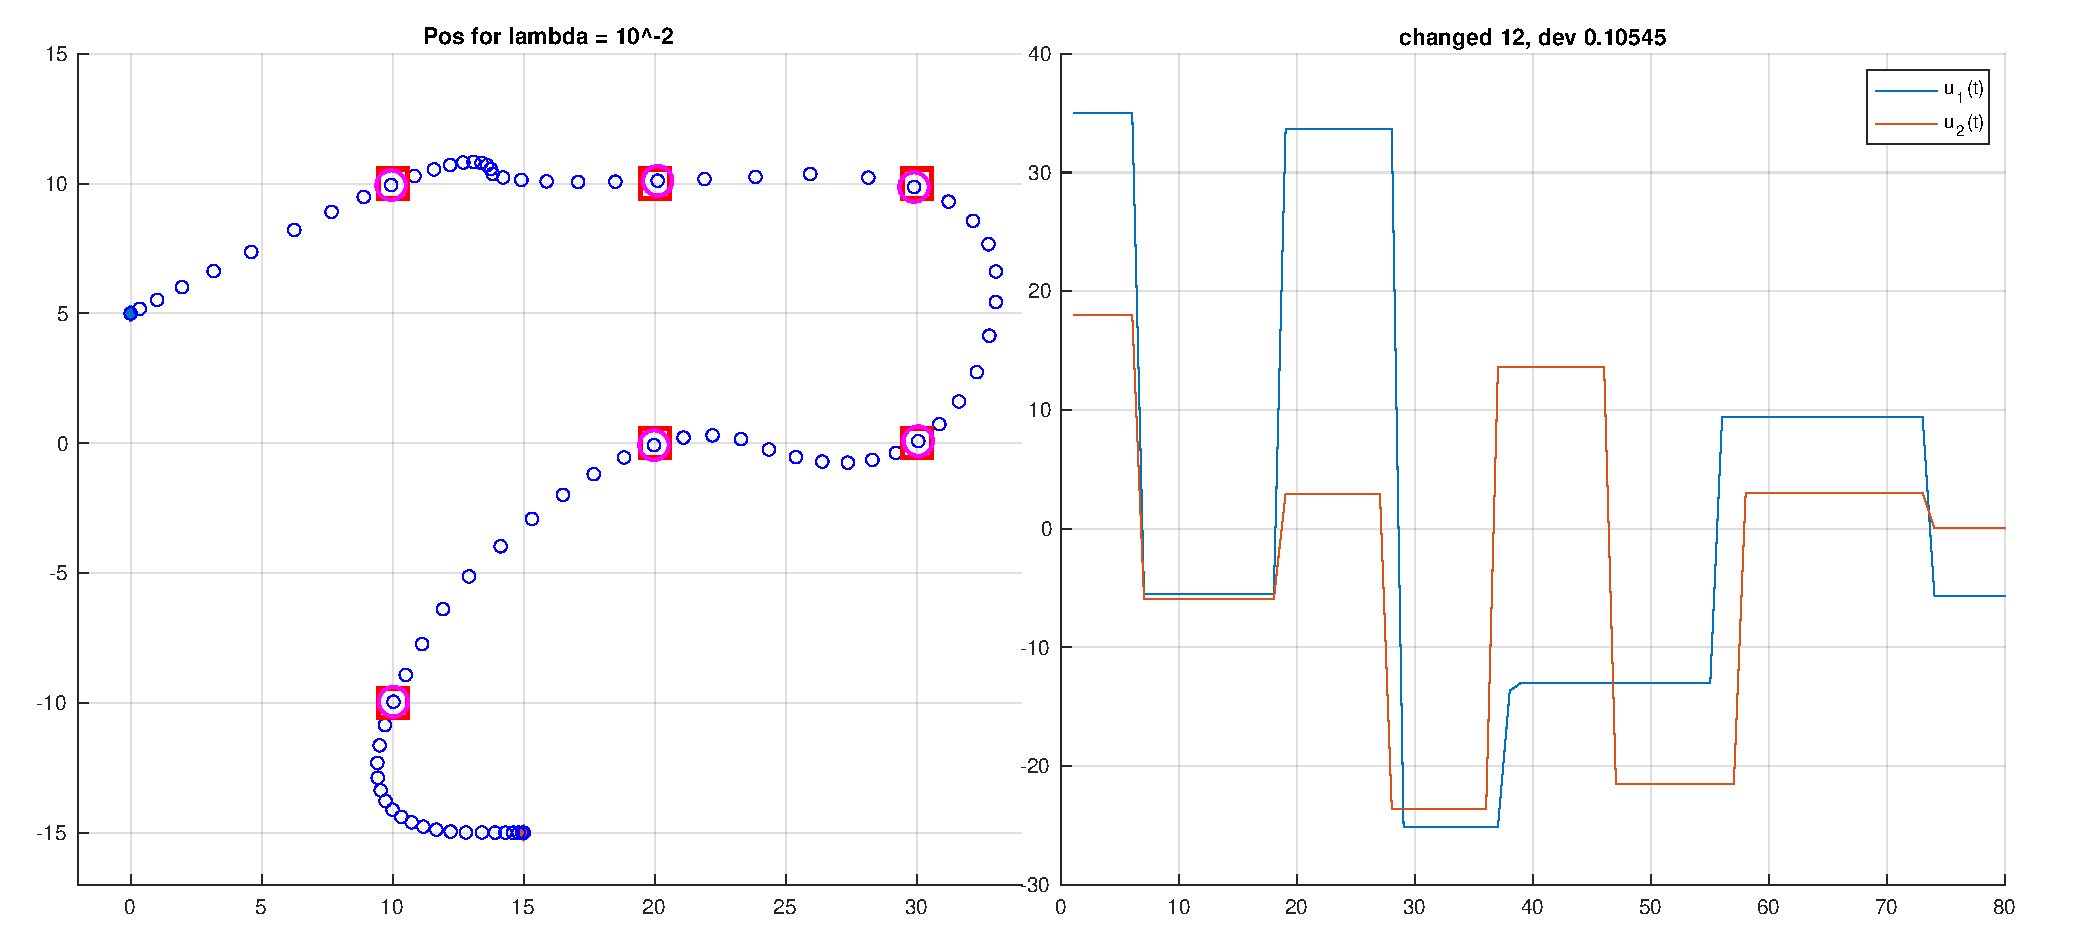
\includegraphics[width=0.5\linewidth]{part1/figures/task3/3_-2.pdf}
\end{subfigure}
\begin{subfigure}
    \centering
    \makebox[\linewidth]{%
        \hspace*{4px}
        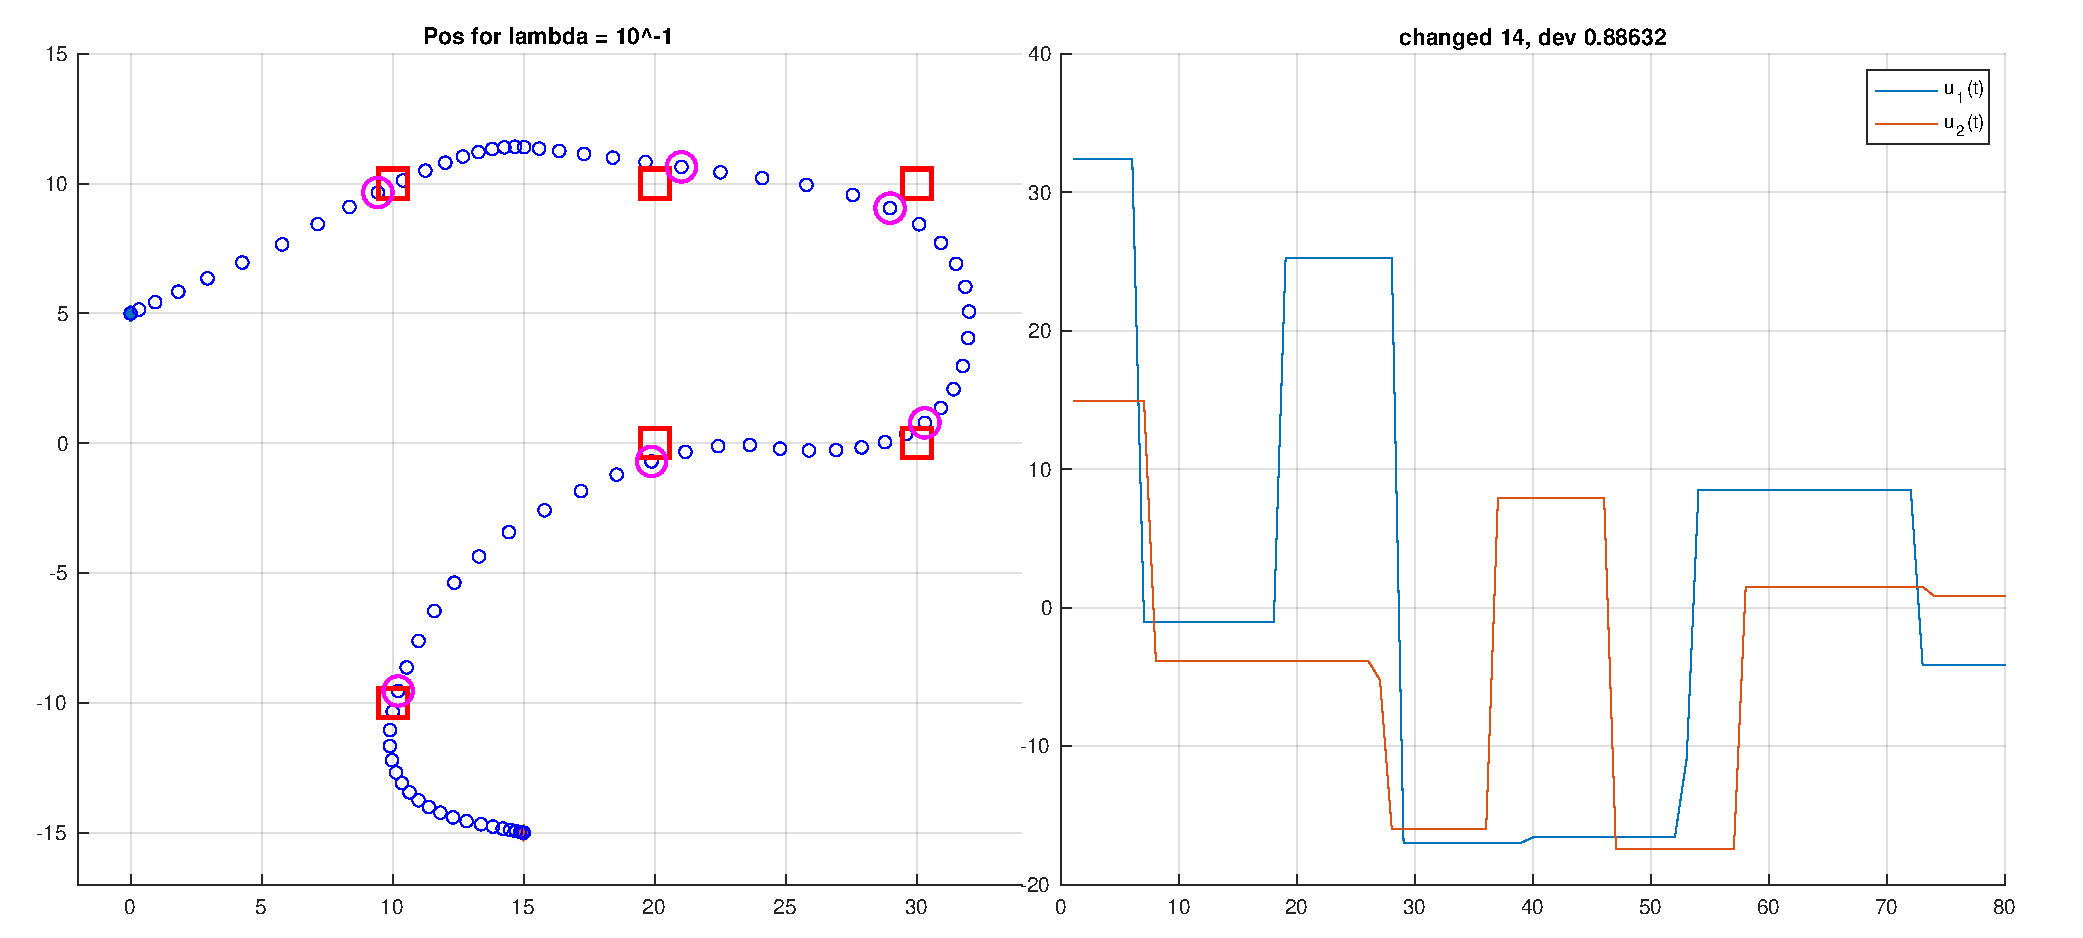
\includegraphics[width=\linewidth + 22px]{part1/figures/task3/3_-1.pdf}
    }
\end{subfigure}
\begin{subfigure}
    \centering
    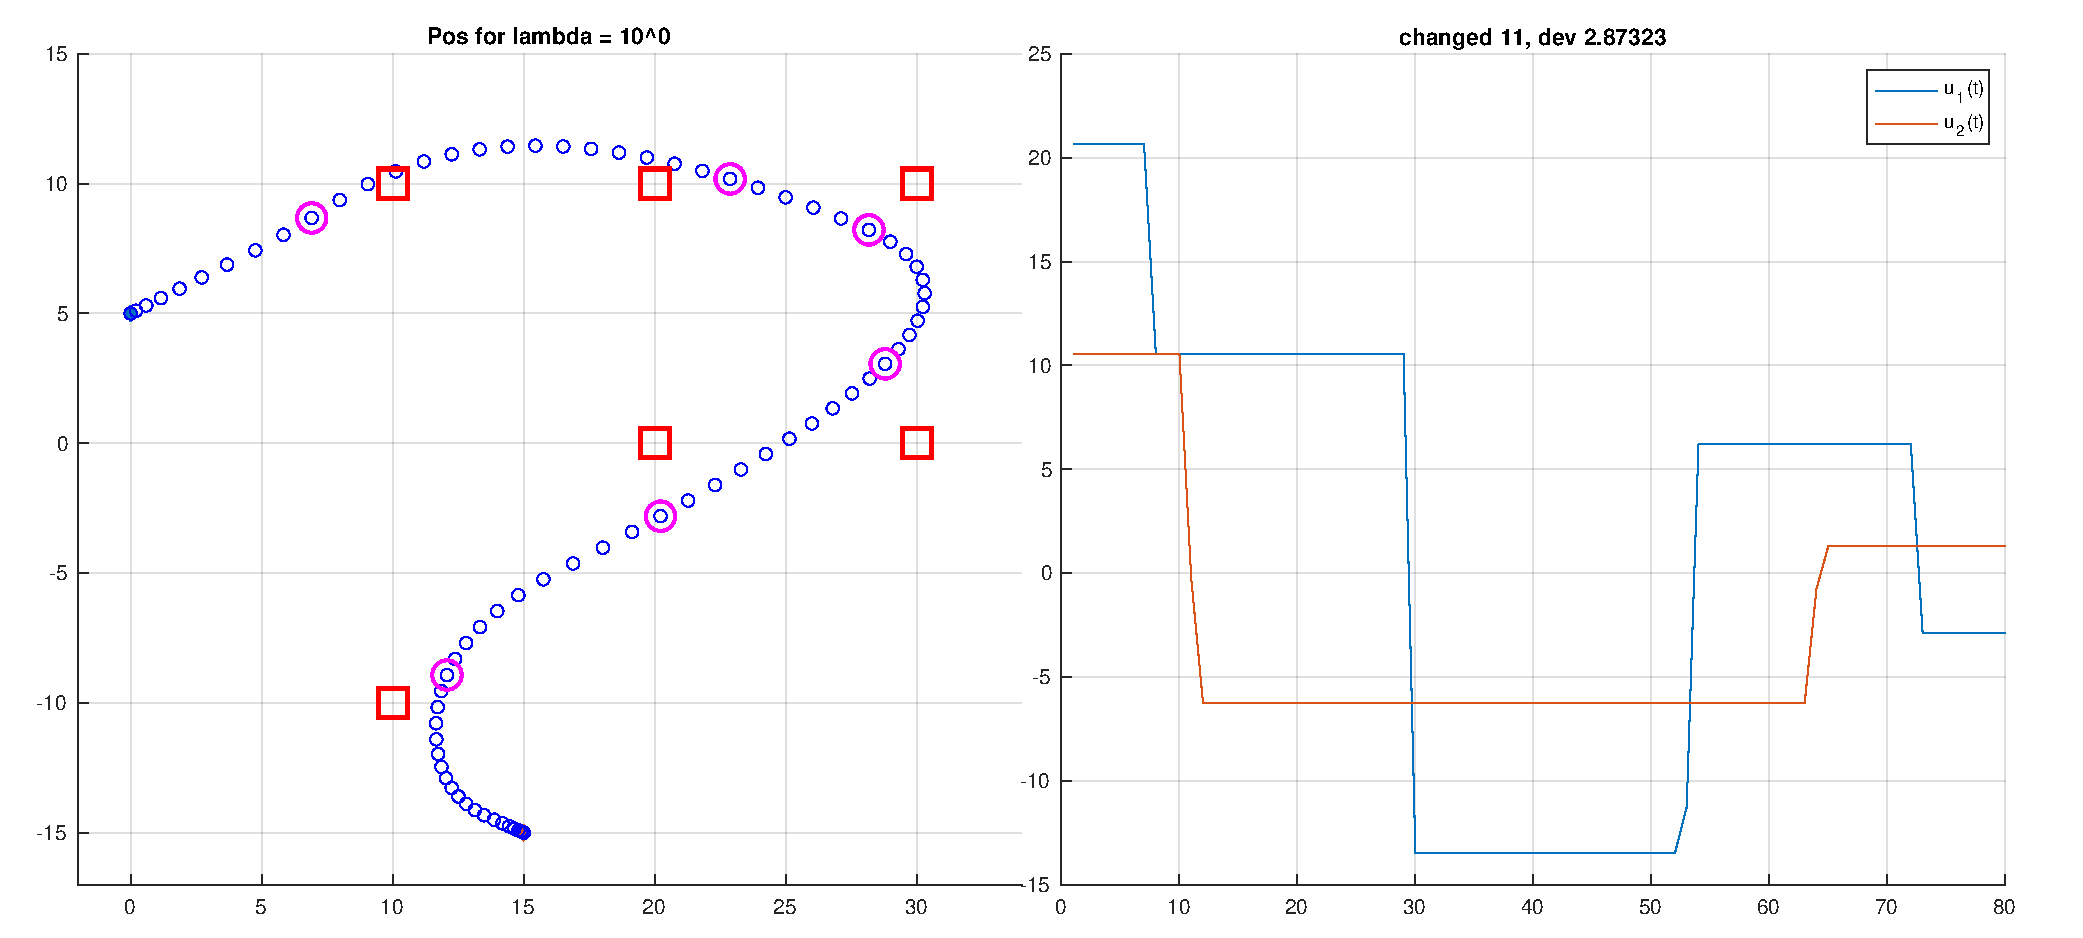
\includegraphics[width=0.5\linewidth]{part1/figures/task3/3_0.pdf}\hspace{0em}
    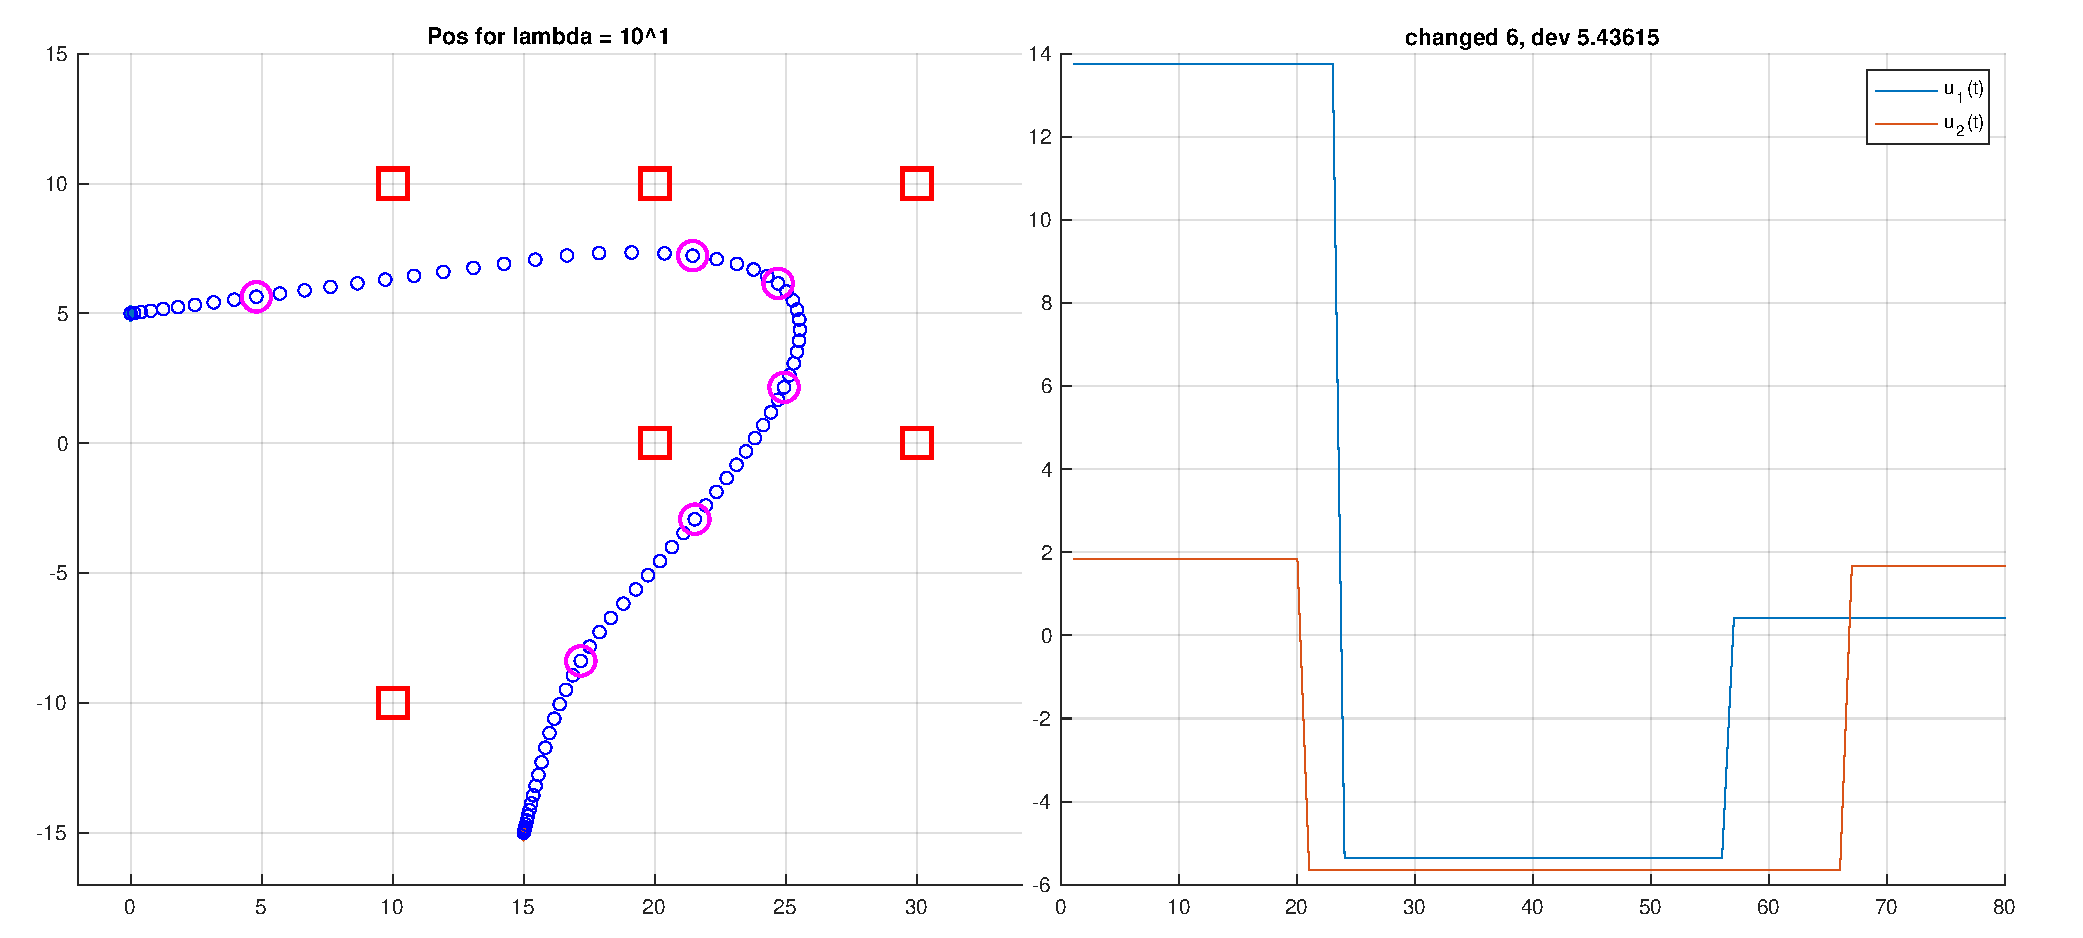
\includegraphics[width=0.5\linewidth]{part1/figures/task3/3_1.pdf}
\end{subfigure}
\begin{subfigure}
    \centering
    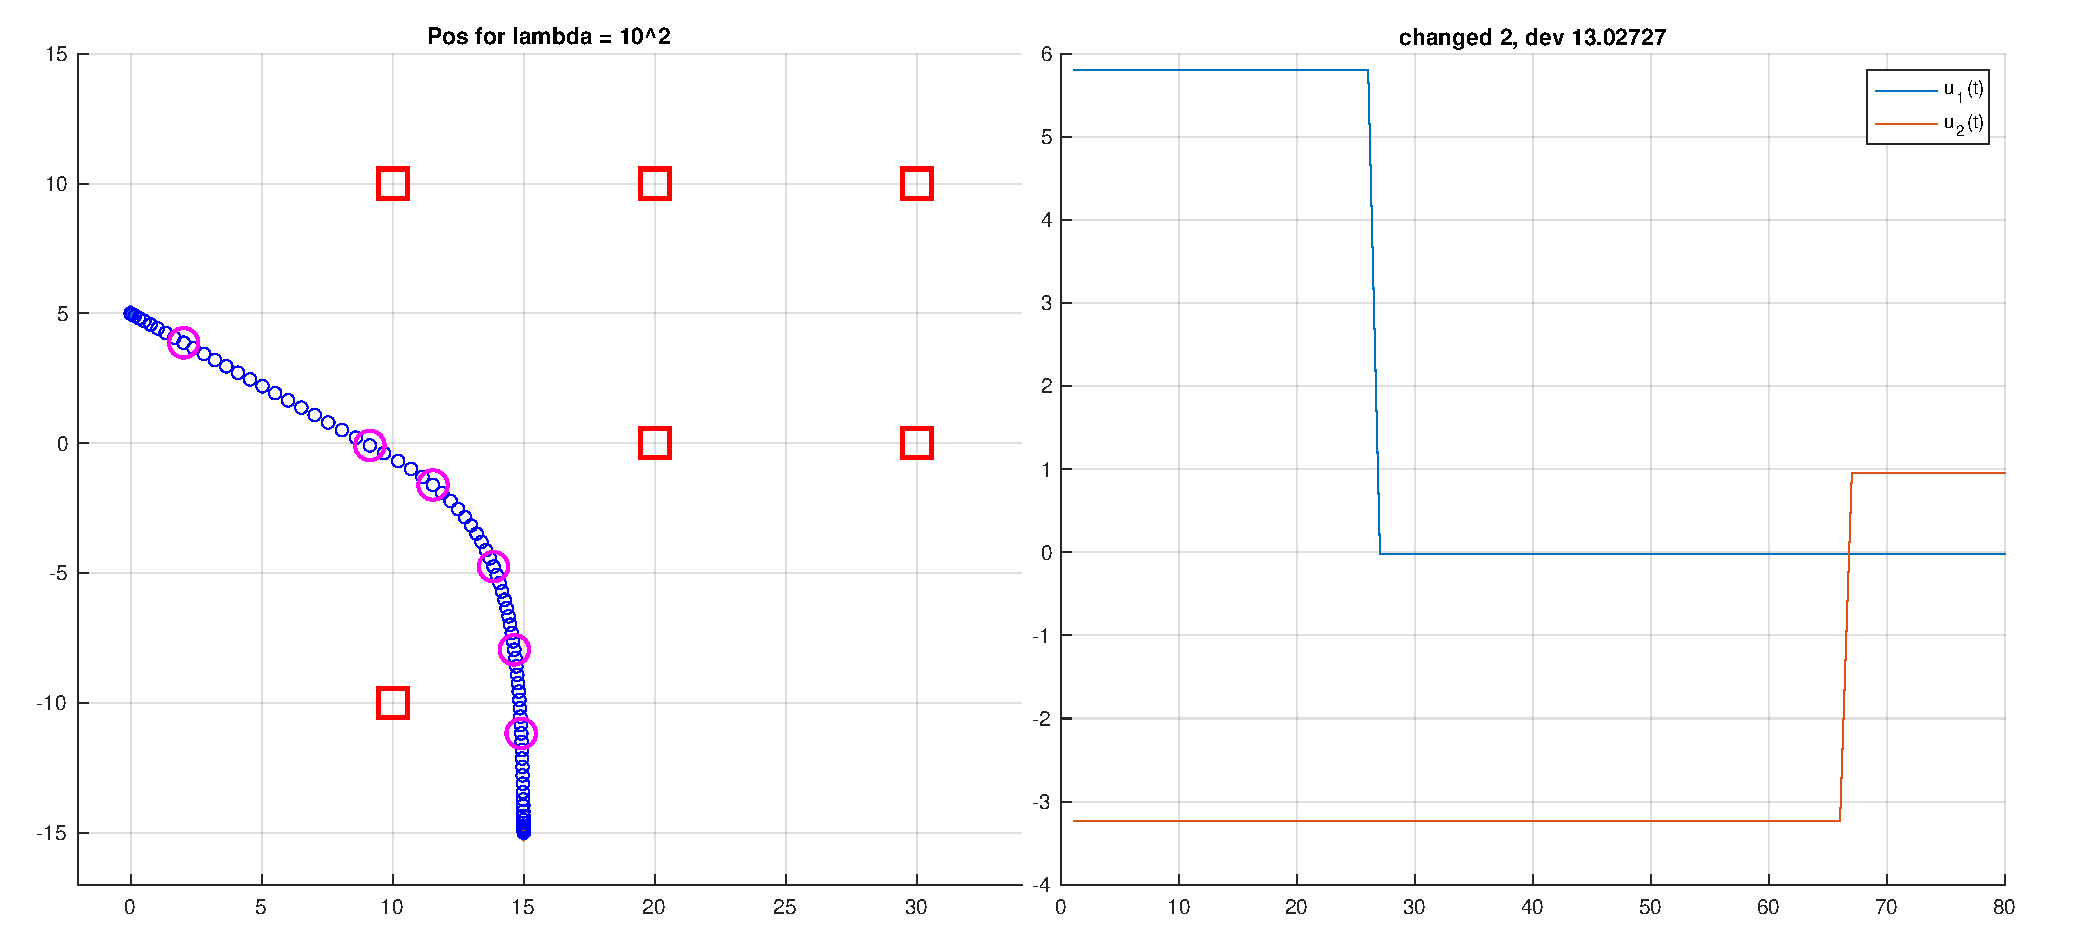
\includegraphics[width=0.5\linewidth]{part1/figures/task3/3_2.pdf}\hspace{0em}
    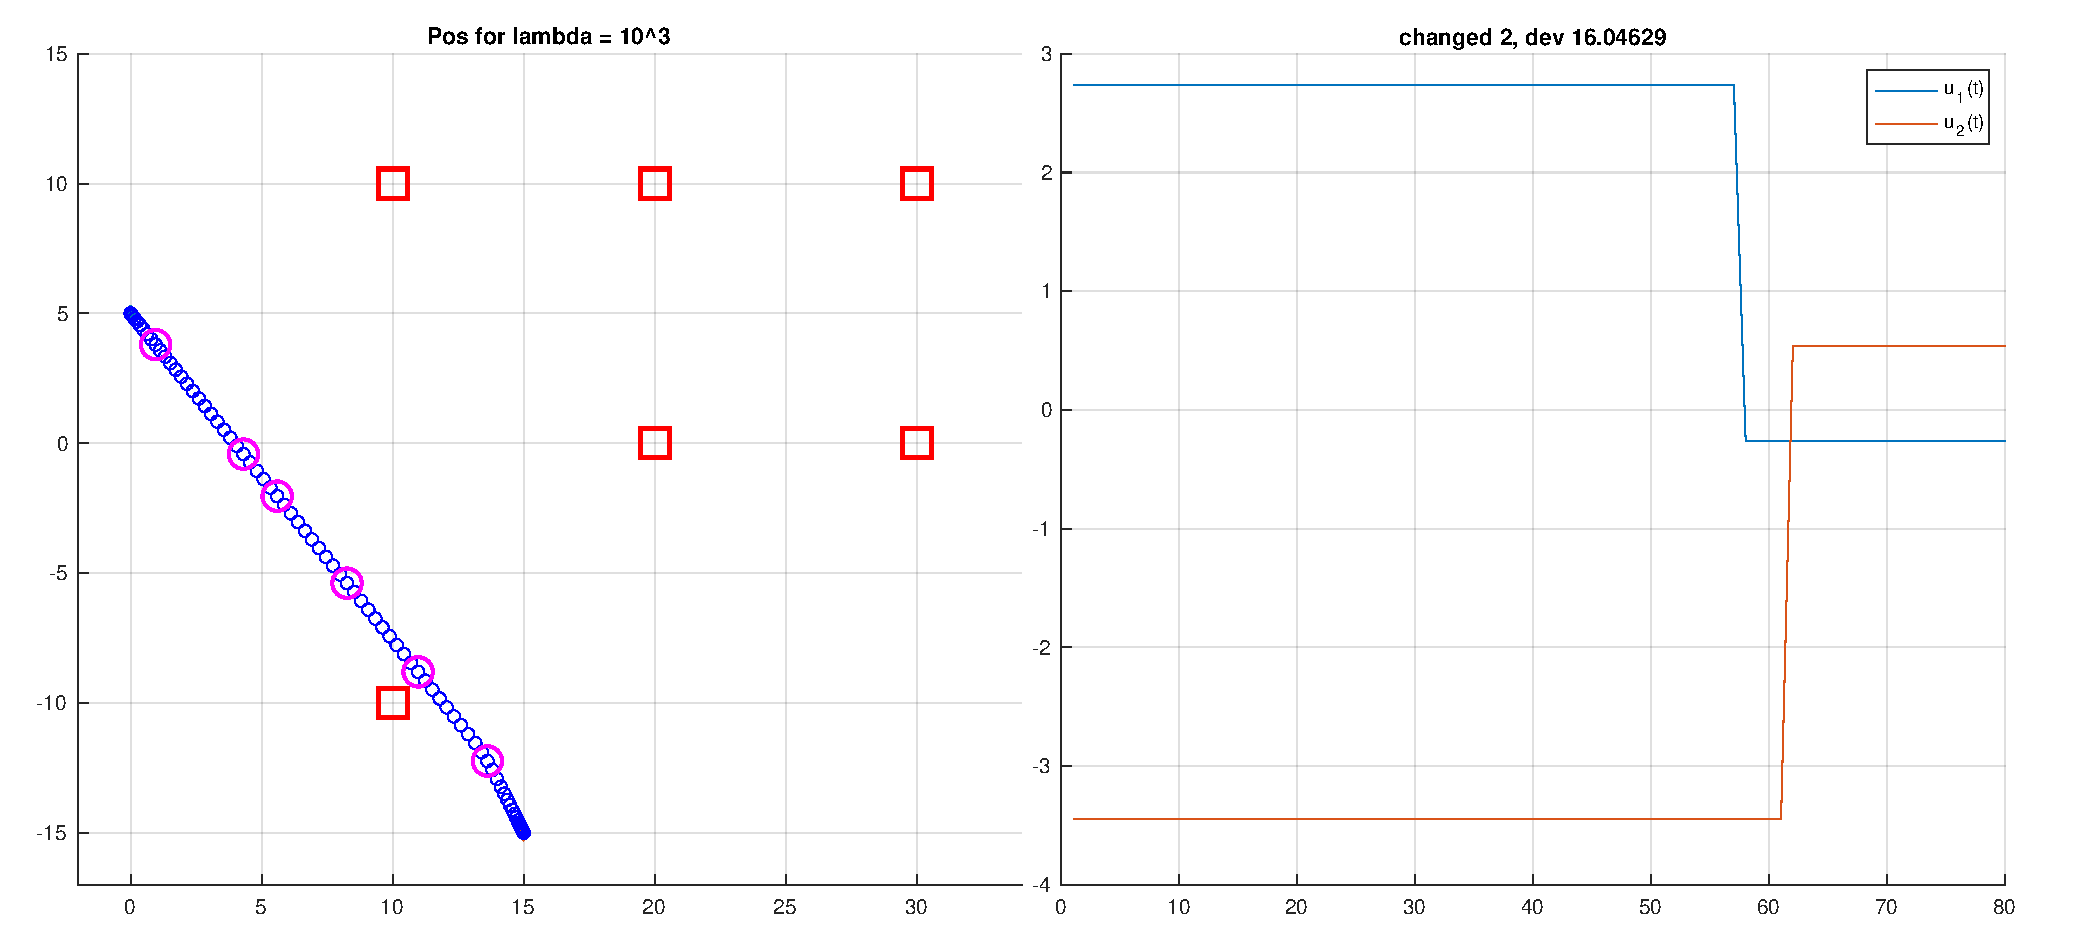
\includegraphics[width=0.5\linewidth]{part1/figures/task3/3_3.pdf}
\end{subfigure}
\end{figure}

\section{Task 4}
%\noindent\fcolorbox{black}{lightgray}{
%    \parbox{\textwidth}{ \textbf{Task 4.} Comment on what you have observed from Tasks 1 to 3 (for example, compare the impact of the three regularizers on the optimal control signal that they each induce).
%    }
%}


\begin{table}[!htb]
    \caption*{Mean deviation and effect of the regularizer based on the $\lambda$ in Tasks 1 to 3.}
    \begin{minipage}{.33\linewidth}
        \centering
        \caption{Task 1 results.}
        \label{task1:table:results}
        \begin{tabular}{c|cr}
            $\lambda$ & changes & m. dev. \\
            \hline
            $10^{-3}$ & 79 & 0.1257 \\
            $10^{-2}$ & 79 & 0.8242 \\
            $10^{-1}$ & 79 & 2.1958 \\
            $10^{+0}$ & 79 & 3.6826 \\
            $10^{+1}$ & 79 & 5.6317 \\
            $10^{+2}$ & 79 & 10.9041 \\
            $10^{+3}$ & 79 & 15.3304
        \end{tabular}
    \end{minipage}%
    \begin{minipage}{.33\linewidth}
      \centering
        \caption{Task 2 results.}
        \label{task2:table:results}
        \begin{tabular}{c|cr}
            $\lambda$ & changes & m. dev. \\
            \hline
            $10^{-3}$ & 10 & 0.0075 \\
            $10^{-2}$ & 8 & 0.0747 \\
            $10^{-1}$ & 11 & 0.7021 \\
            $10^{+0}$ & 5 & 2.8876 \\
            $10^{+1}$ & 4 & 5.3689 \\
            $10^{+2}$ & 3 & 12.5914 \\
            $10^{+3}$ & 1 & 16.2266
        \end{tabular}
    \end{minipage}%
    \begin{minipage}{.33\linewidth}
      \centering
        \caption{Task 3 results.}
        \label{task3:table:results}
        \begin{tabular}{c|cr}
            $\lambda$ & changes & m. dev. \\
            \hline
            $10^{-3}$ & 13 & 0.0107 \\
            $10^{-2}$ & 12 & 0.1055 \\
            $10^{-1}$ & 14 & 0.8863 \\
            $10^{+0} $ & 11 & 2.8732 \\
            $10^{+1} $ & 6 & 5.4361 \\
            $10^{+2} $ & 2 & 13.0273 \\
            $10^{+3} $ & 2 & 16.0463
        \end{tabular}
    \end{minipage} 
\end{table}

The objective function which we try to minimize in the tasks 1 to 3 consists of sum of two parts. The first part, common to all of three tasks measures how far away the robot is from the waypoints at given times. This is defined as $\sum_{k = 1}^K \left\| E x( \tau_k ) - w_k \right\|_2^2$. 

Second part of the objective function, the regularizer, differs among the first three tasks. Regularizer enforces the fourth wish (simple control) by penalizing the deviations of the control signal from its previous value. By changing the $\lambda$ parameter, we can change the importance of this wish. If the $\lambda$ becomes a large number, the objective function's value shifts towards the regularizer which enforces least number of changes to the control signal. Making the $\lambda$ a large value naturally increases the mean deviation as we put larger importance to minimizing the number of changes of the control signal instead of capturing all of the points.

\noindent
\begin{minipage}{.33\linewidth}
    \begin{equation}
        \label{task1:regularizer}
        \sum_{t = 1}^{T-1} \left\| u(t) - u(t-1) \right\|_2^2
    \end{equation}
\end{minipage}
\begin{minipage}{.33\linewidth}
    \begin{equation}
        \label{task2:regularizer}
        \sum_{t = 1}^{T-1} \left\| u(t) - u(t-1) \right\|_2
    \end{equation}
\end{minipage}
\begin{minipage}{.33\linewidth}
    \begin{equation}
        \label{task3:regularizer}
        \sum_{t = 1}^{T-1} \left\| u(t) - u(t-1) \right\|_1
    \end{equation}
\end{minipage}

Effect of this behavior is shown in the Figure \ref{fig:task4:waypoint:dev}. The number of changes in the control signal does not change for the Task 1 as it stays $79$. The number of changes for Task 2 and 3 is visualized in the Figure \ref{fig:task4:changes}.


\begin{figure}[!htb]
    \centering
    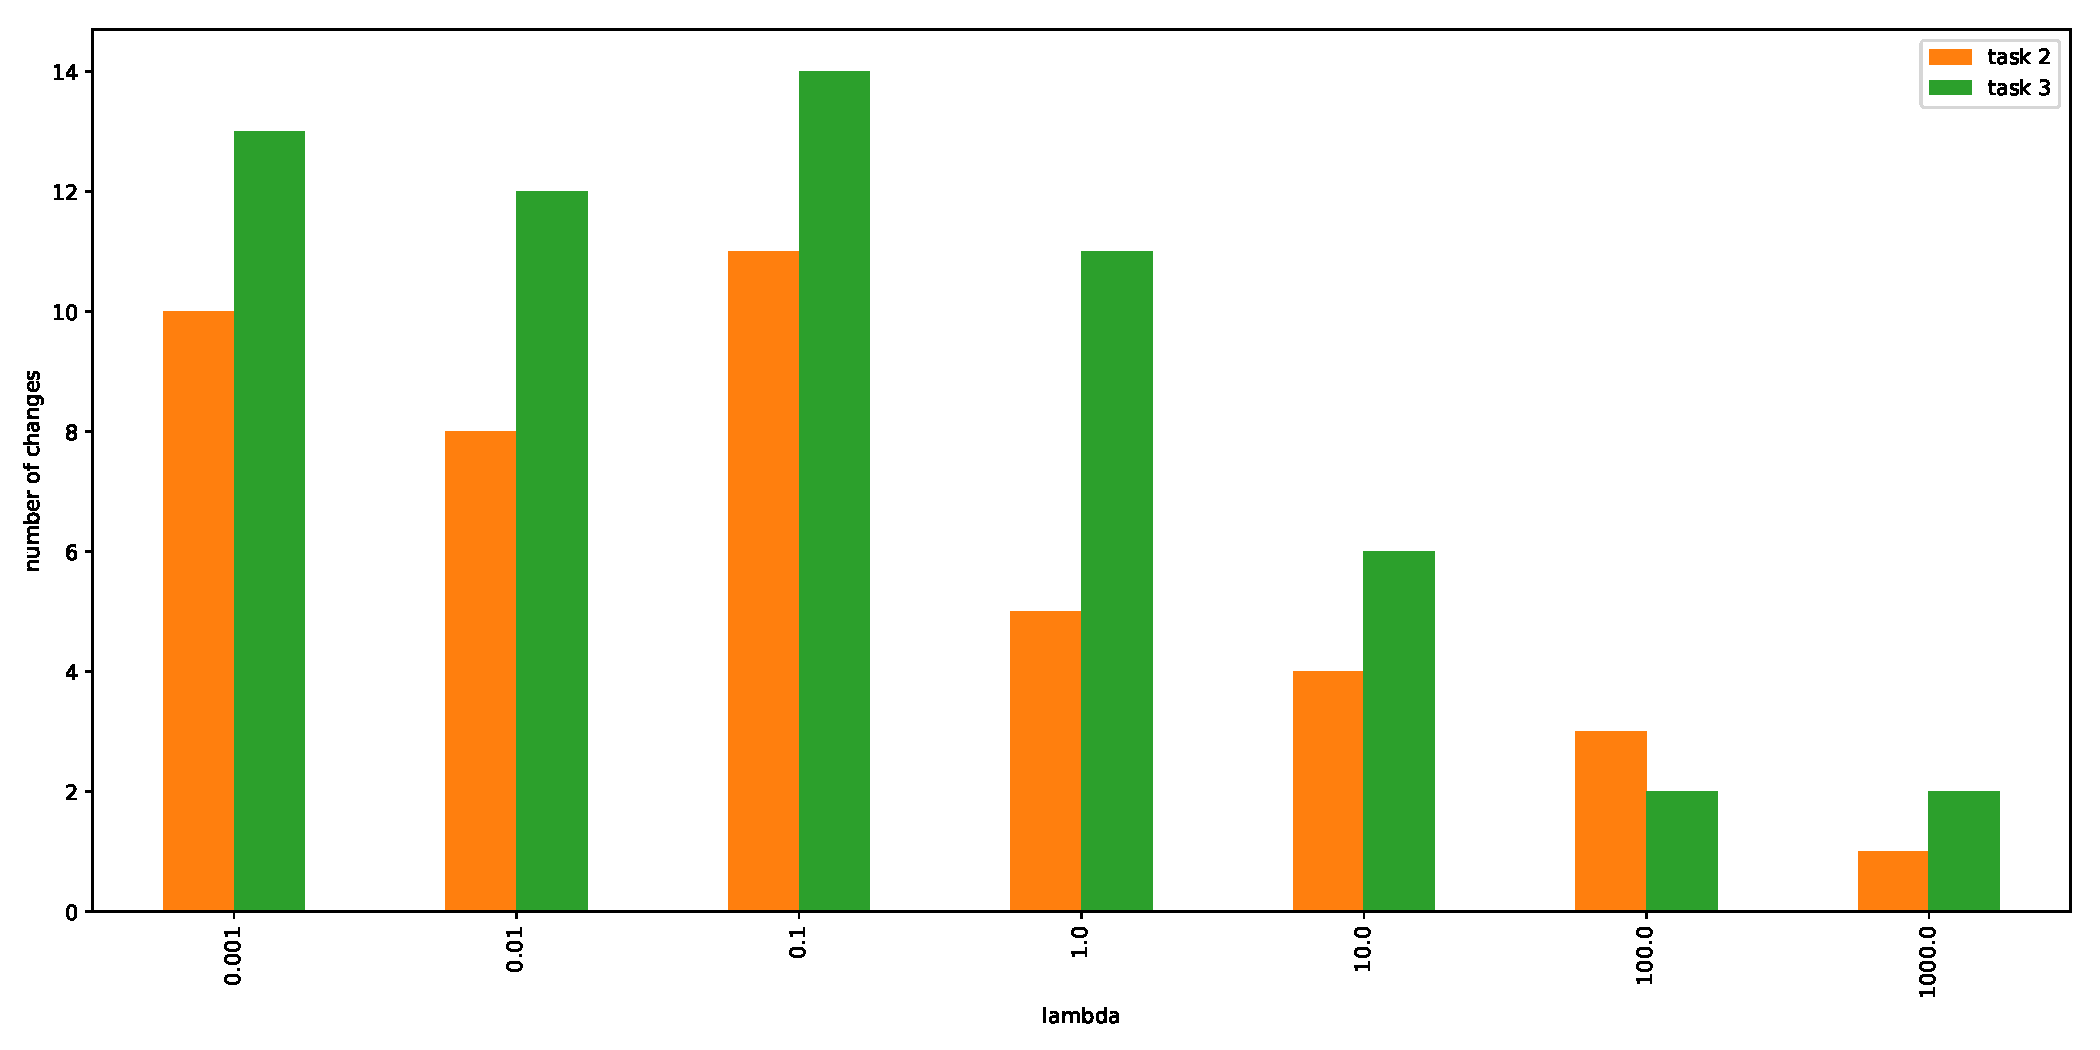
\includegraphics[width=\linewidth]{part1/notebooks/task_2_3_signal_changes.pdf}
    \caption{Control signal changes for Tasks 2 and 3.}
    \label{fig:task4:changes}
\end{figure}


\begin{itemize}
    \item[\textbf{Task 1}] utilizes the squared L2 regularizer as shown in Equation \ref{task1:regularizer}. Benefit of using the squared L2 norm can be in easier computation, as no square root needs to be computed. The differences between control signals are absolutely limited by the \textit{U\_Max} constraint which results in them being often number lower than 1. Squaring a small number leads to even smaller value. Since the value is too small, the contribution to the objective function is neglected and the optimizer rather minimizes the captured waypoints. 
    \item[\textbf{Task 2}] utilizes the L2 norm, described in Equation \ref{task2:regularizer}. This can be interpreted as a euclidean distance from the previous actuator vector to the current one. Calculating the square root of a small value ($<0$) makes this value larger. The contribution to the objective function is therefore larger than in the Task 1. The lowest number of updates (1) was achieved by using the $\lambda=10^3$. We can see, that the control signal's function is no longer smooth, but rather has a form of squares as the robot utilizes large control signals which change rarely.
    \item[\textbf{Task 3}] relies on the L1 norm, as described in Equation \ref{task3:regularizer}. This norm is not differentiable at 0, however it induces a behavior which was called ``L1 magic'' - the property of producing many coefficients with zero values or very small values with few large coefficients\footnote{http://www.chioka.in/differences-between-the-l1-norm-and-the-l2-norm-least-absolute-deviations-and-least-squares/}.
\end{itemize}

Surprisingly, the performance of the L2 norm in this task is superficial to the L1 norm as the robot achieves lower mean deviation with the same number of points captured. 

\begin{figure}[!htb]
    \centering
    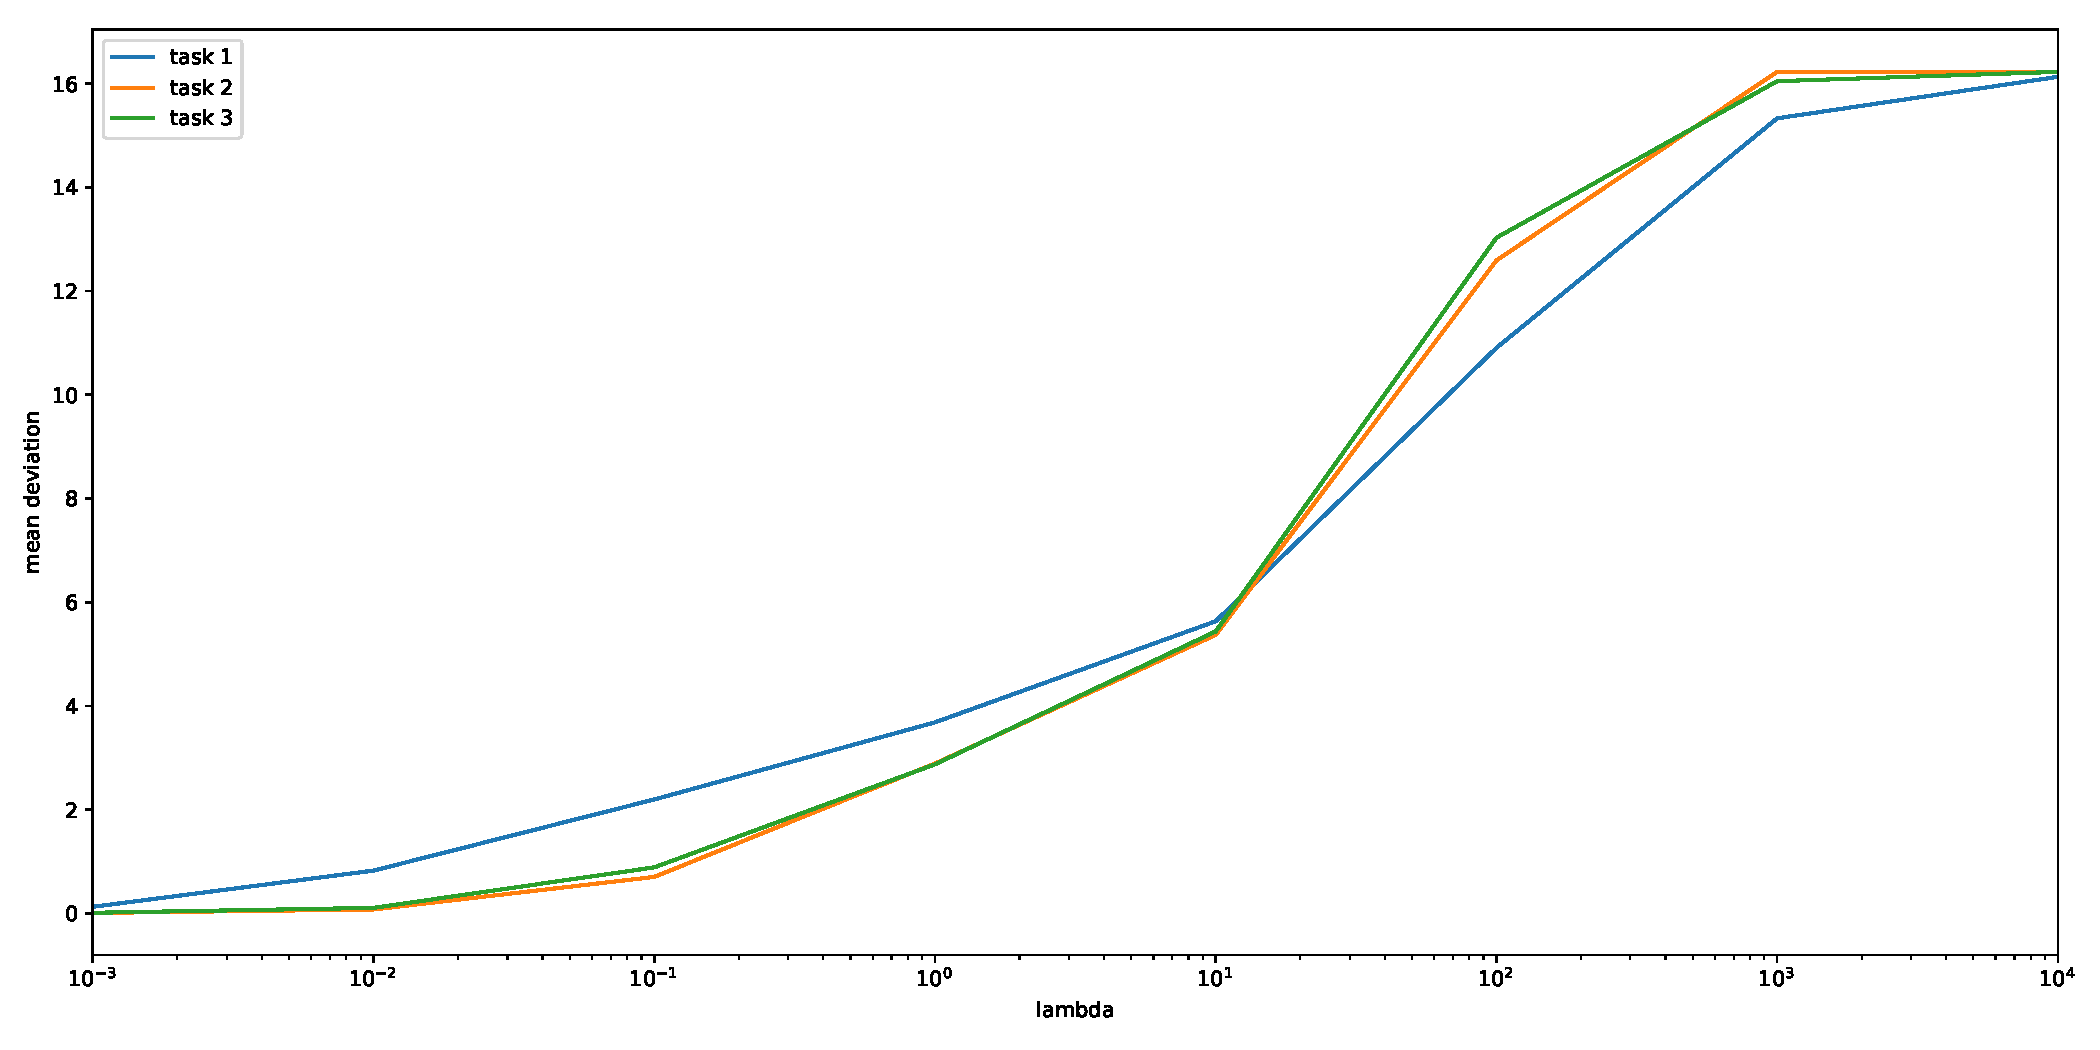
\includegraphics[width=\linewidth]{part1/notebooks/task_1_2_3_waypoint_mean_dev.pdf}
    \caption{Waypoint mean deviation for Tasks 1 to 3.}
    \label{fig:task4:waypoint:dev}
\end{figure}

\section{Task 5}
%\noindent\fcolorbox{black}{lightgray}{
%    \parbox{\textwidth}{ \textbf{Task 5.} Using simple geometric arguments, give a  closed-form expression for $d\left( p,D(c,r) \right)$.
%    }
%}

Distance between point $p$ and disc $D\left(c, r\right)$ is defined as:
\begin{equation}
    d\left(p,D\left(c,r\right)\right) = \textit{min}\{\left\|p-y\right\|: y \in D\left(c, r\right)\}
\end{equation}

Based on whether the point is within the disc or not, the following cases might occur:
\begin{equation}
	d\left( p,D(c,r) \right) = 
	\begin{cases} 
		0                           & \text{if } \left\|p - c\right\|_2 \leq r\\ 
		\left\|p - c\right\|_2 - r 	& \text{if } \left\|p - c\right\|_2 > r
	\end{cases}
\end{equation}

If the result of $\left\|p - c\right\|_2 - r$ is negative, the point is within the circle and the distance should be 0. If the point is outside of the disc, then the result is equal to $\left\|p - c\right\|_2 - r$. Based on this, we conclude that the equation can be written in a closed form as:
\begin{equation}
    % \textit{max}\left(0, \left\|p(\tau_{k}), c_{k}\right\|_2 - r_k \right)
	d\left(p,D\left(c,r\right)\right) = \textit{max}\left(0, \left\|p - c\right\|_2 - r \right)
\end{equation}

\section{Task 6}
%\noindent\fcolorbox{black}{lightgray}{
%    \parbox{\textwidth}{ \textbf{Task 6.} Use the software ${\tt CVX}$ to solve problem~\eqref{P:prob4}. After you solve the problem, do the following:
%    \begin{enumerate}[(a)]
%    \item plot the optimal positions of the robot from $t = 0$ to $t = T$, marking its positions at the appointed times $\tau_k$, for $1 \leq k \leq K$;
%    \item plot the optimal control signal $u(t)$, where $u(t) = ( u_1(t), u_2(t) )$, from $t = 0$ to $t = T-1$;
%    \item report how many times the optimal control signal changes from $t = 1$ to $t = T-1$; 
%    \item report the mean deviation from the waypoints (defined in~\eqref{meanwaydev});     
%    \item comment on the results from (a)-(d), as you compare them with those you obtained in Task 1. (Note that Task 1 considered waypoints, which can be seen as disks with radius zero.)
%    \end{enumerate}
%    }
%}

% comment on the results from (a)-(d), as you compare them with those you obtained in Task 1. (Note that Task 1 considered waypoints, which can be seen as disks with radius zero.

Mean deviation and number of changes for the Task 6 is shown in the Table \ref{table:task6:table}. The resulting robot's optimal positions are shown in the Figure \ref{fig:task6:figure}.

\begin{table}[!htb]
    \centering
    \caption{Mean deviation and number of changes for 6.}
    \label{table:task6:table}
    \begin{tabular}{c|ccr}
        $\lambda$ & changes & circle m. dev. & center m. dev. \\
        \hline
        $10^{-1}$ & 8 & 0 & 1.4142
    \end{tabular}
\end{table}

\begin{figure}[!htb]
    \centering    
    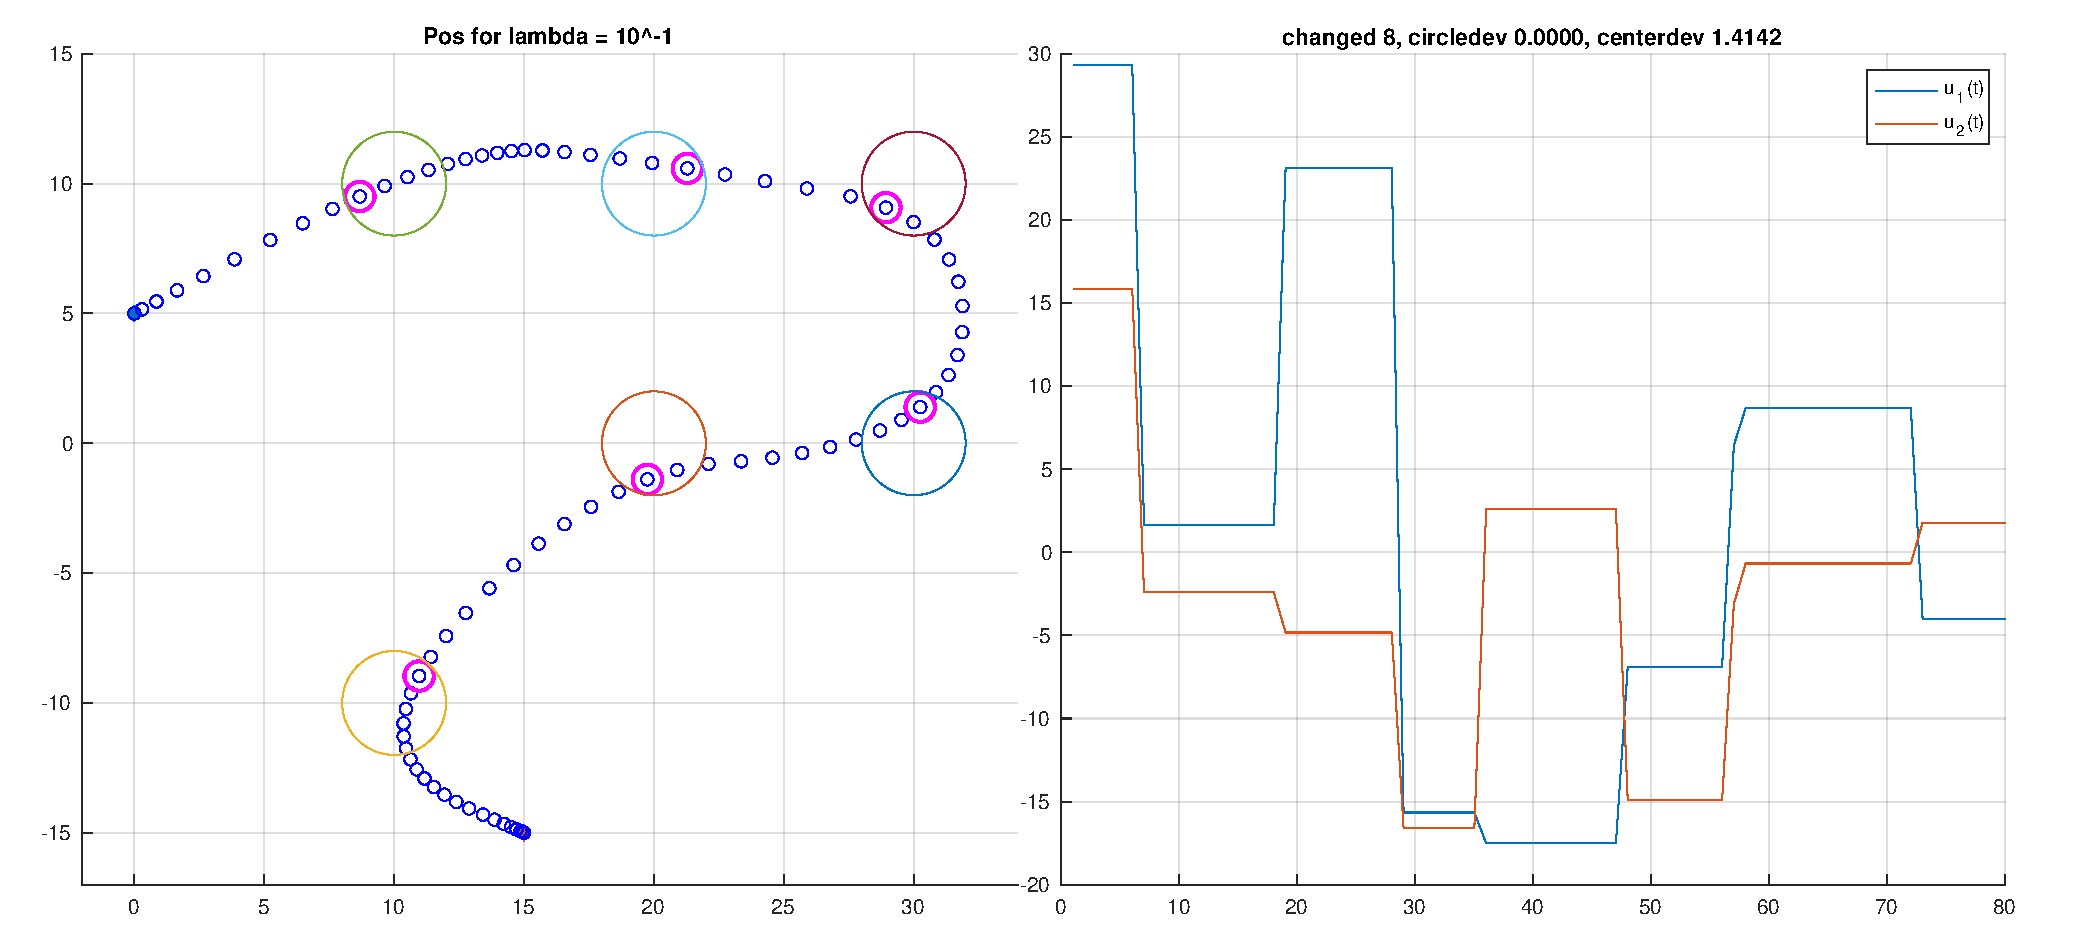
\includegraphics[width=1\linewidth]{part1/figures/task_6.pdf}
    \caption{Robot positions and control signal for Task 6.}
    \label{fig:task6:figure}
\end{figure}



\section{Task 7}
%\noindent\fcolorbox{black}{lightgray}{
%    \parbox{\textwidth}{ \textbf{Task 7.} Use the software ${\tt CVX}$ to solve problem~\eqref{P:prob5a}. Explain what happens.}
%}

We implemented the task 7 in CVX code as shown in the listing \ref{listing:task7:cvx}. The variables are same as in the previous exercises with the exception of $\text{U\_Max}=15$.

\begin{lstlisting}[language=Matlab, caption=CVX code for task 7., label=listing:task7:cvx, float=!htb]
cvx_begin
    variable x(4,T+1);
    variable u(2,T);
    minimize(0);
    subject to
        % Initial and end speed need to be 0
        x(:,1)     == [p_initial; [0; 0]];
        x(:,T+1)   == [p_final;   [0; 0]];
        % Make sure that the robot moves using the constrains
        x(:,2:T+1) == A*x(:,1:T) + B*u(:,1:T);
        % Check the actuator force size
        for ux = u
            norm(ux, 2) <= U_max; 
        end
        % Enforce the correct positions of the robot
        for ti = 1:length(tau)
            E*x(:, tau(ti)) ==  w(:, ti);
        end
cvx_end
\end{lstlisting}

The CVX tries to solve this task, but fails to do so and reports the following:
\begin{lstlisting}
Status: Infeasible
Optimal value (cvx_optval): +Inf
\end{lstlisting}

This indicates, that CVX has not found a feasible solution to the given constrains. This is likely due to the actuator force $\text{U\_Max}=15$ being too low. 

We have investigated setting the \text{U\_Max} as another CVX variable and optimizing it with \lstinline{minimize(U_max)} which returns $38.8989$. We can see, that with value of $\text{U\_Max}=38.8989$ this feasibility problem has a solution.

\section{Task 8}
The function $\phi$ outputs a zero if its argument is zero and outputs a one, otherwise. That is, we have $\phi\,:\,{\mathbf R}^2 \rightarrow {\mathbf R}$, with $$\phi(x) = \left\{ \begin{array}{ll} 0,  & \text{ if } x = 0, \\ 1, & \text{ if }x \neq 0. \end{array} \right.$$

%\noindent\fcolorbox{black}{lightgray}{
%    \parbox{\textwidth}{ \textbf{Task 8.} Show that the function $\phi$ is nonconvex.}
%}

\begin{equation}
	\forall x_1, x_2 \in X, \forall t \in [0, 1]: \qquad f(tx_1+(1-t)x_2)\leq t f(x_1)+(1-t)f(x_2)
\end{equation}

Function f is convex if for any two points $x_{1}, x_{2}$ ant $t\in[0, 1]$ the above inequality is true. We select $x_{1} = 0$, $x_{2} = 1$ and $t=0.5$. The inequality for this setting and function $\phi$ is described below.

\begin{equation}
\begin{split}
	\phi(t \cdot x_1+(1-t) \cdot x_2) &\leq t \cdot \phi(x_1)+(1-t) \cdot \phi(x_2)\\
	\phi(0.5 \cdot 0 + 0.5 \cdot 1) &\leq 0.5 \cdot \phi(0) + 0.5 \cdot f(1)\\
	\phi(0.5) &\leq 0.5 \cdot \phi(0) + 0.5 \cdot f(1)\\
	1 &\leq 0.5
\end{split}
\end{equation}

As we can see above, this inequality is a contradiction for selected $x_{1}$, $x_{2}$ and t. Since $\phi$ does not fulfill the requirements for a convex function, we conclude that it is non convex.

\section {Task 9}
%\noindent\fcolorbox{black}{lightgray}{
%    \parbox{\textwidth}{ \textbf{Task 9.} Use the software ${\tt CVX}$ to solve problem~\eqref{P:prob6}. After you solve the problem, do the following:
%    \begin{enumerate}[(a)]
%    \item plot the optimal positions of the robot from $t = 0$ to $t = T$, marking its positions at the appointed times $\tau_k$, for $1 \leq k \leq K$;
%    \item plot the optimal control signal $u(t)$, where $u(t) = ( u_1(t), u_2(t) )$, from $t = 0$ to $t = T-1$;
%    \item report how many waypoints are captured by the robot; consider that a waypoint $w_k$ is captured if the robot is sufficiently close to it at the appointed time $\tau_k$, namely, if $\left\| p( \tau_k) - w_k \right\|_2 \leq 10^{-6}$.
%    \end{enumerate}
%    }
%}

The minimized function can be expressed in CVX as shown on Listing \ref{listing:task9:cvx}.

\begin{lstlisting}[language=Matlab, caption=CVX code for task 9., label=listing:task9:cvx]
minimize(sum(vec_sqr_sum(E*x(:,tau+1) - w)));
\end{lstlisting}

The robot positions are shown in the Figure \ref{fig:task9:graph}. The robot did not capture any point.

\begin{figure}[!htb]
    \caption{Robot positions and control signal for Task 9.}
    \label{fig:task9:graph}
    \centering    
    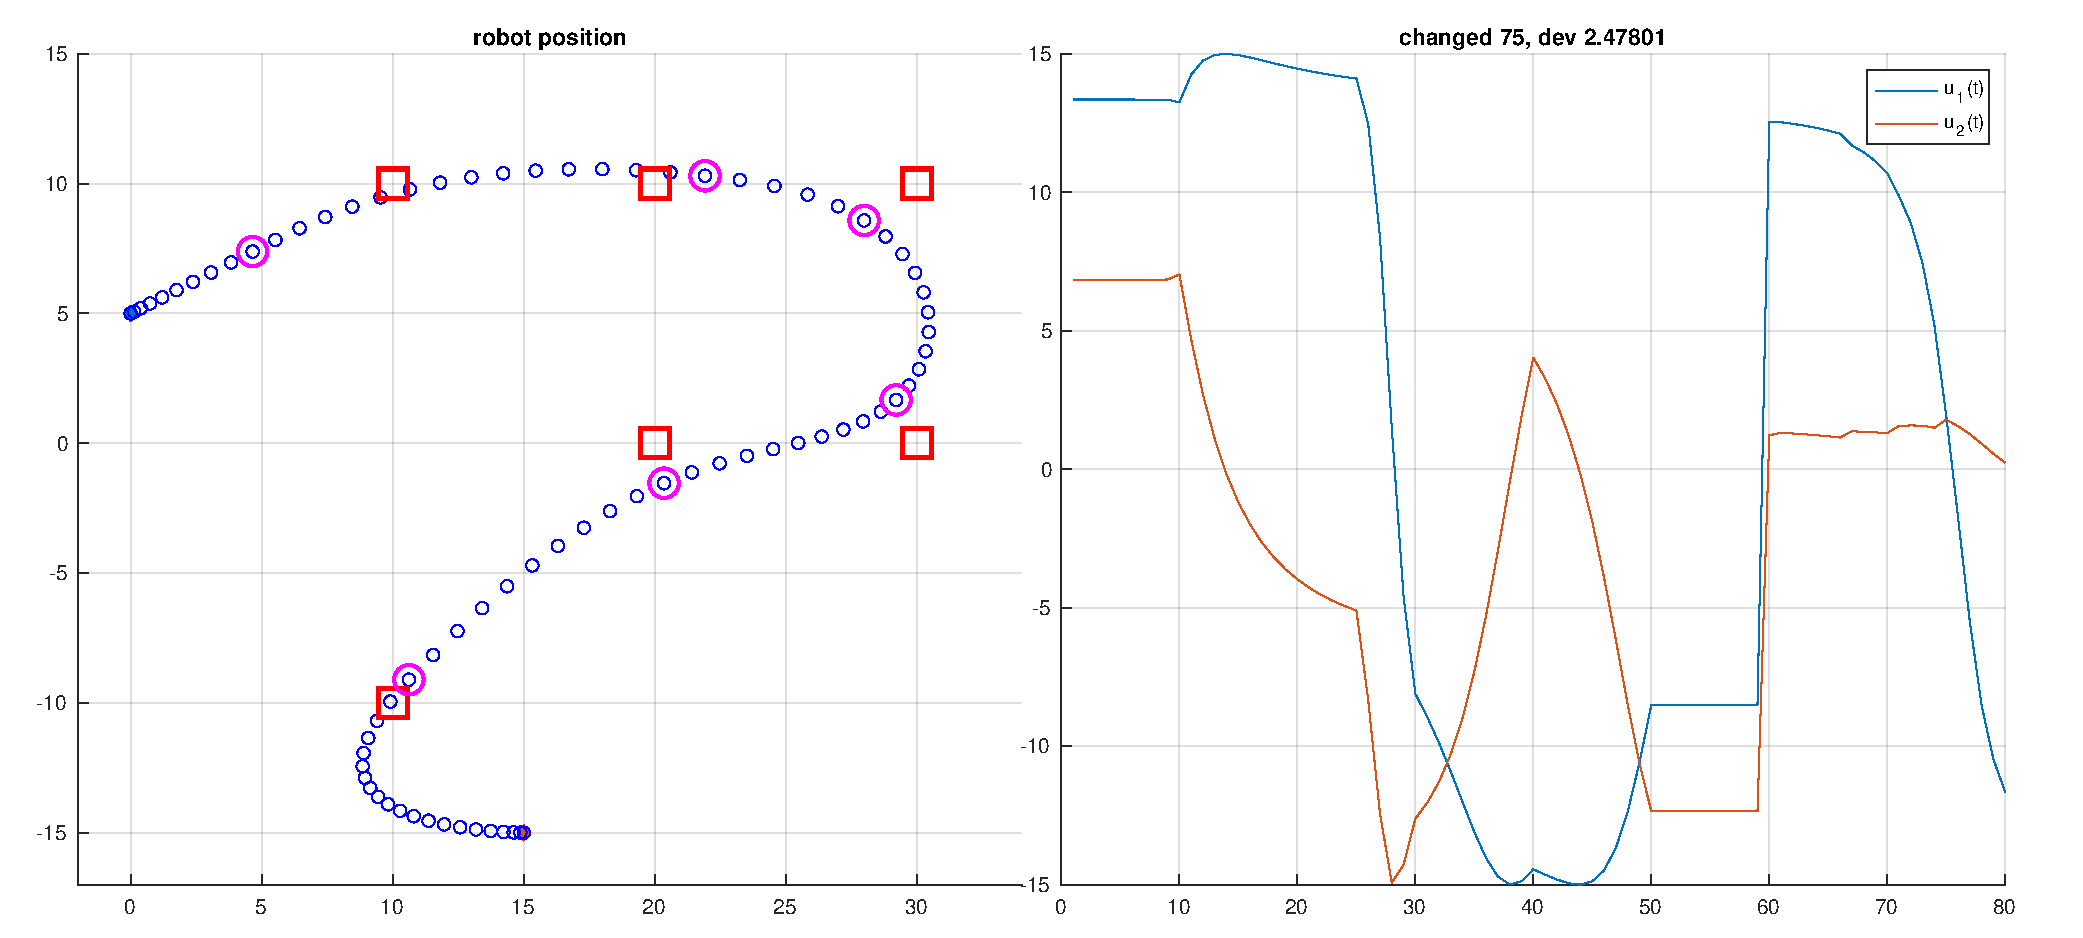
\includegraphics[width=1\linewidth]{part1/figures/task_9.pdf}
\end{figure}

\section {Task 10}
%\noindent\fcolorbox{black}{lightgray}{
%    \parbox{\textwidth}{ \textbf{Task 10.} Redo task 9 for problem~\eqref{P:prob7}.
%    }
%}

The minimized function can be expressed in CVX as shown on Listing \ref{listing:task10:cvx}. The robot has captured a single point along its journey.

\begin{lstlisting}[language=Matlab, caption=CVX code for task 10., label=listing:task10:cvx]
minimize(sum(norms(E*x(:,tau+1) - w, 2)));
\end{lstlisting}

The resulting robot positions are visualized in the Figure \ref{fig:task10:graph}.

\begin{figure}[!htb]
    \caption{Robot positions and control signal for Task 10.}
    \label{fig:task10:graph}
    \centering    
    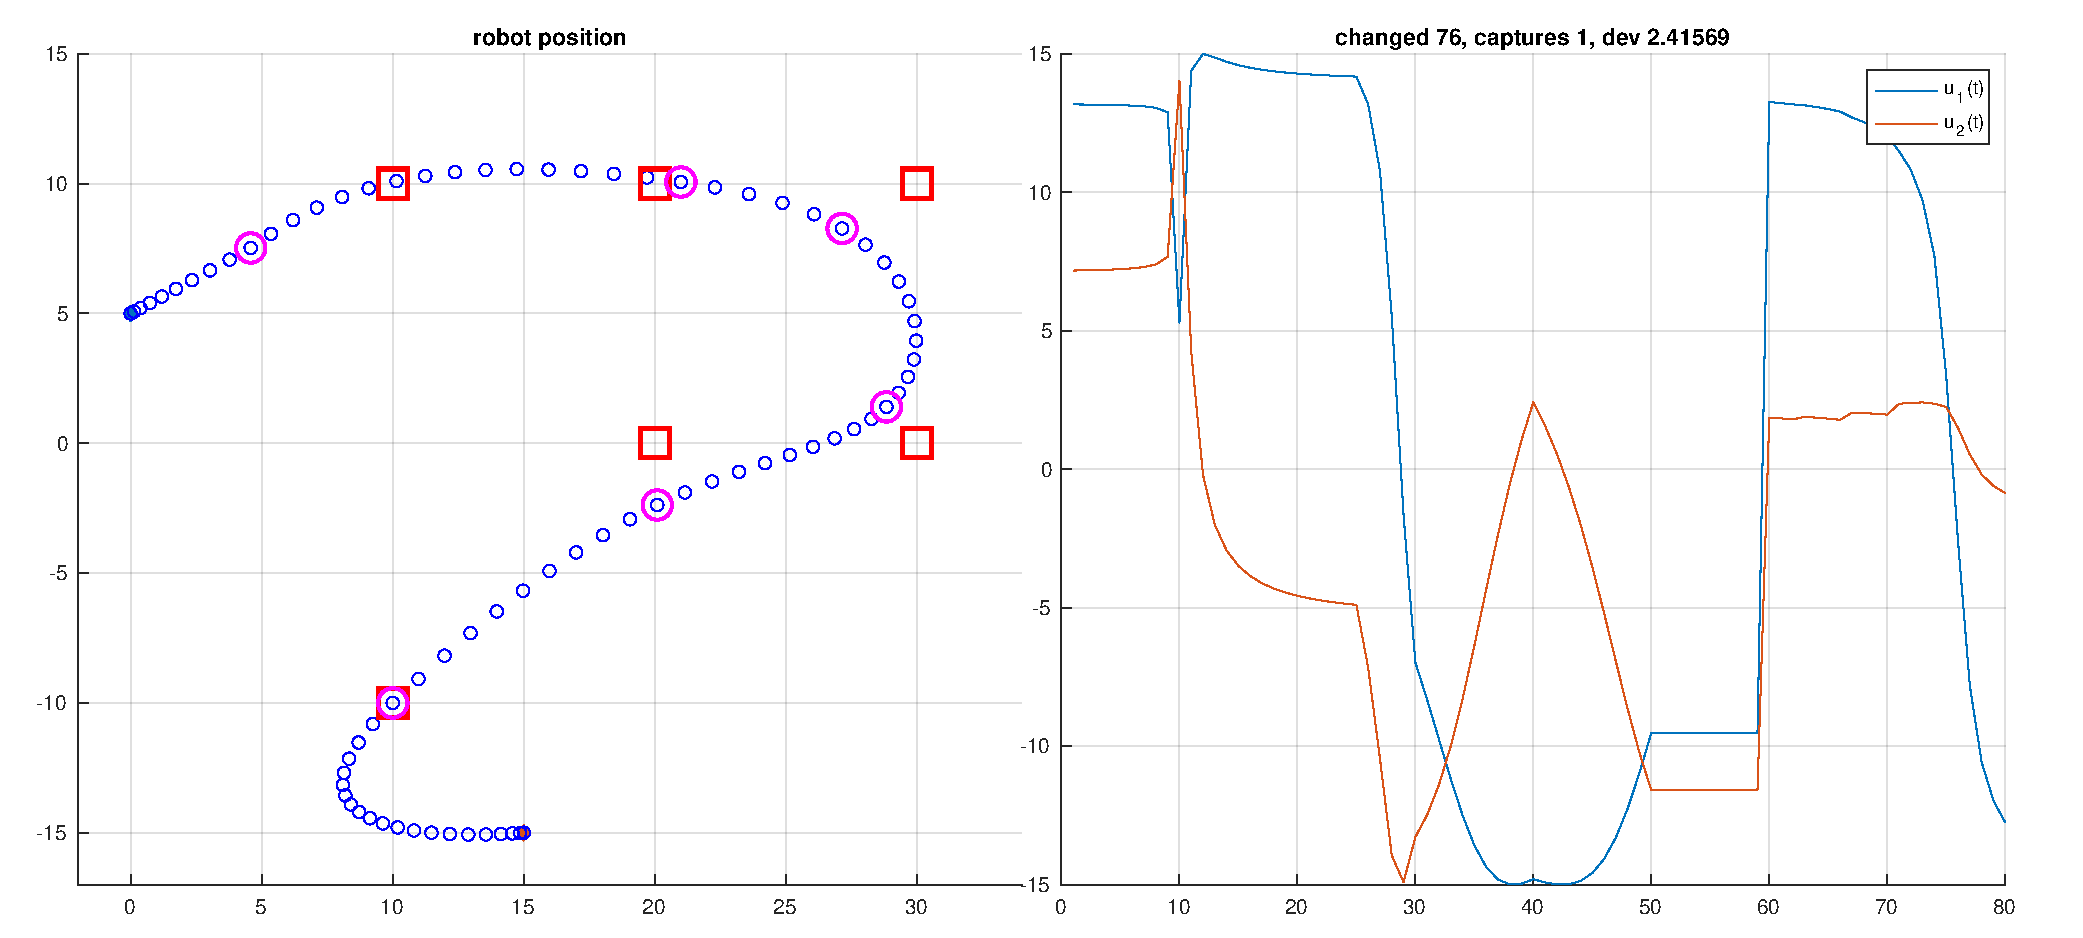
\includegraphics[width=1\linewidth]{part1/figures/task_10.pdf}
\end{figure}

\section {Task 11}
%\noindent\fcolorbox{black}{lightgray}{
%    \parbox{\textwidth}{ \textbf{Task 11.} Apply the reweighting  technique $M$ times, with $M = 10$; that is, solve problem problem~\eqref{P:prob8} for $m = 0, 1, \ldots, M-1$. For each value of $m$, do the following:
%     \begin{enumerate}[(a)]
%    \item plot the positions of the robot in $x^{(m)}$ from $t = 0$ to $t = T$, marking its positions at the appointed times $\tau_k$, for $1 \leq k \leq K$;
%    \item plot the control signal $u^{(m)}(t)$, where $u^{(m)}(t) = \left( u_1^{(m)}(t), u_2^{(m)}(t) \right)$, from $t = 0$ to $t = T-1$;
%    \item report how many waypoints are captured by the robot.
%    \end{enumerate}}
%}

The solution to the reweighting problem is visualized in the Figure \ref{fig:task11:graphs}. The results are described in the Table \ref{table:task11:results}.

\begin{table}[!htb]
\caption{Results of the reweighting technique in Task 11.}
\label{table:task11:results}
\centering
\begin{tabular}{l|ll}
m & captured & mean dev. \\
\hline
0 & 1 & 2.4157 \\
1 & 2 & 2.4567 \\
2 & 2 & 2.5737 \\
3 & 3 & 2.7362 \\
4 & 3 & 2.7355 \\
5 & 3 & 2.7355 \\
6 & 3 & 2.7355 \\
7 & 3 & 2.7355 \\
8 & 3 & 2.7355 \\
9 & 3 & 2.7355
\end{tabular}
\end{table}

\begin{figure}[!htb]
    \caption{Robot positions and control signal for Task 11.}
    \label{fig:task11:graphs}
    \begin{subfigure}
        \centering
        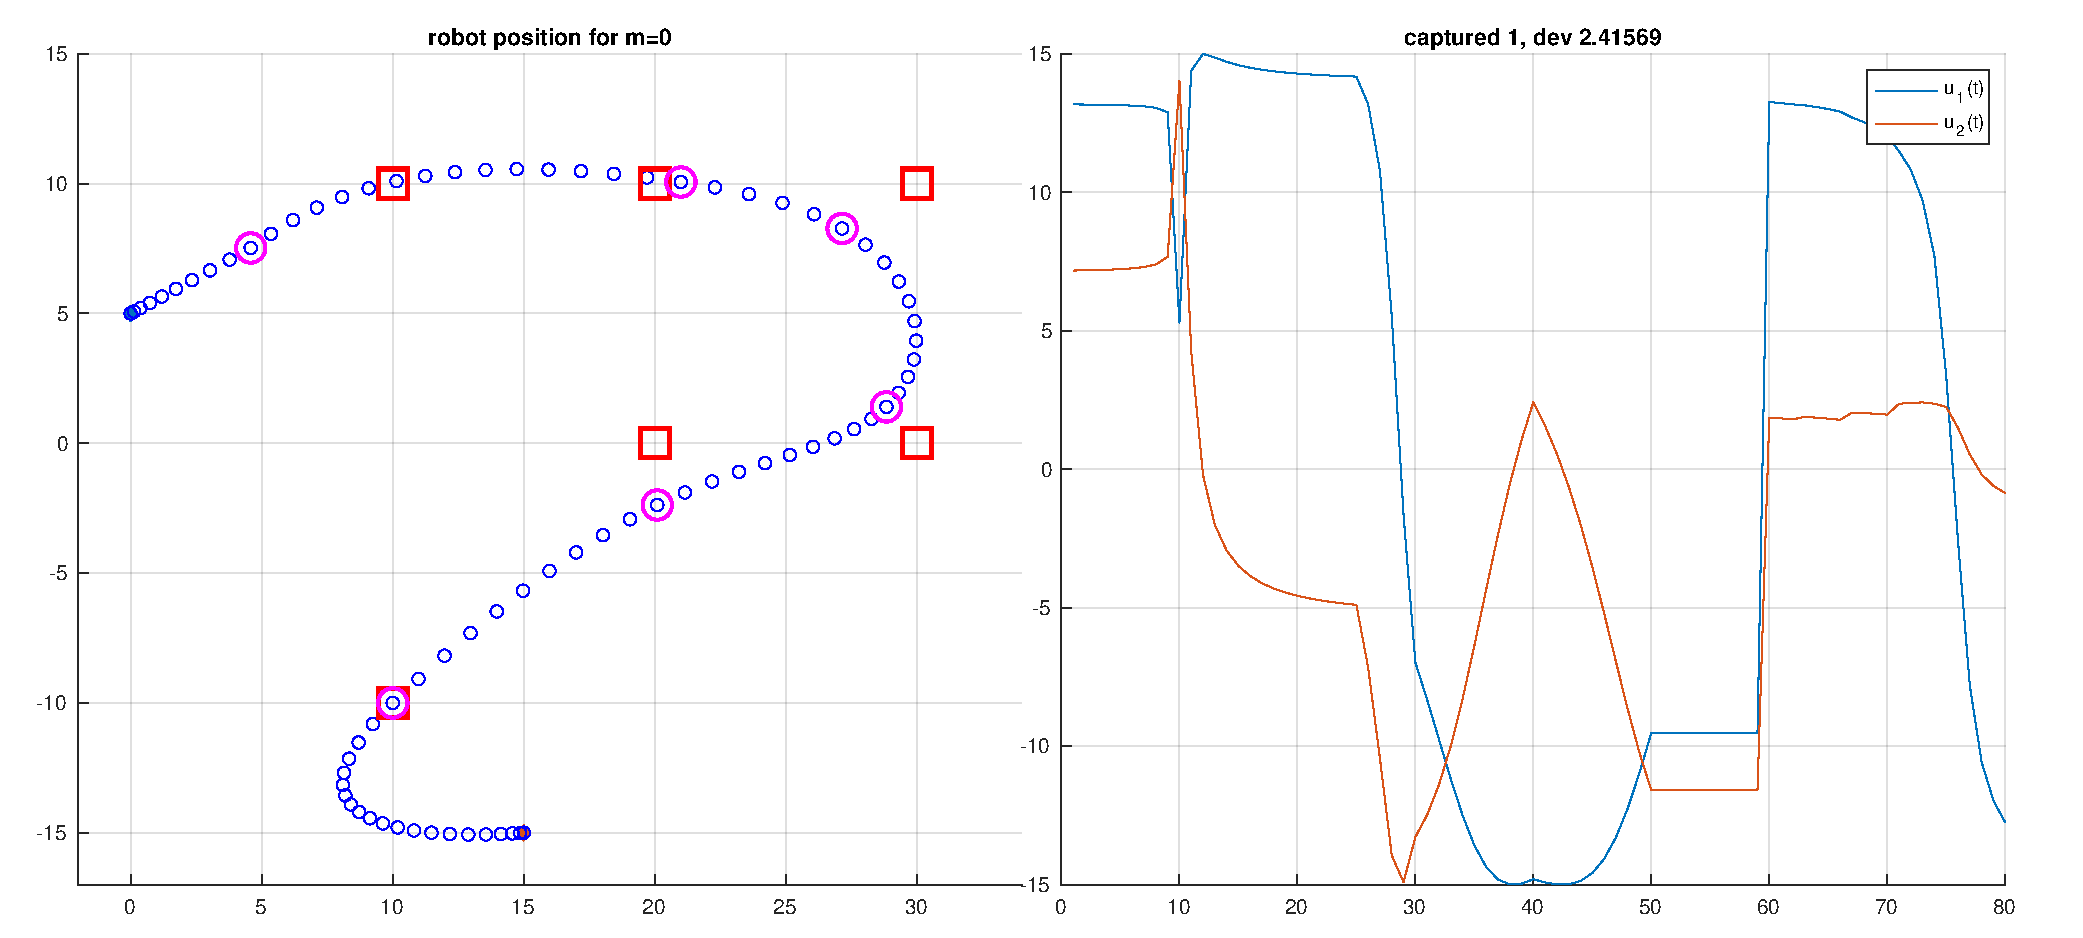
\includegraphics[width=0.5\linewidth]{part1/figures/task11/task_11_0.pdf}\hspace{0em}
        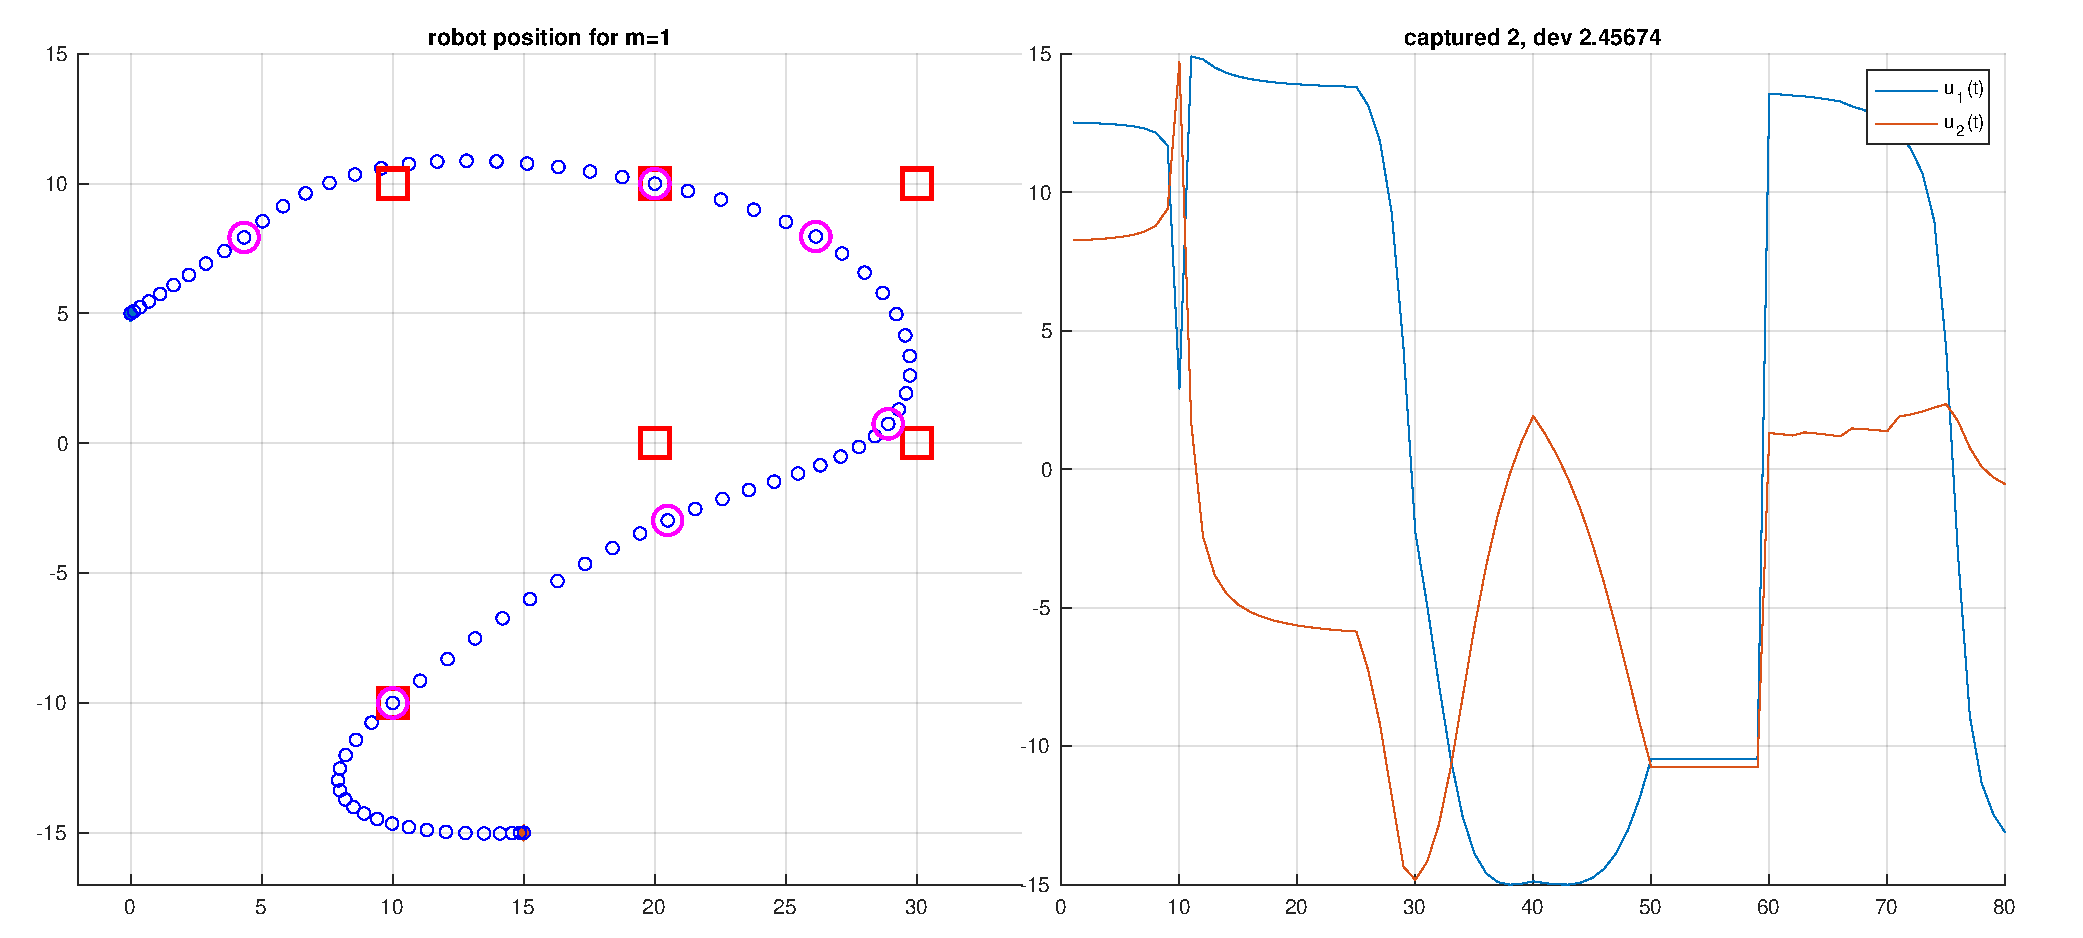
\includegraphics[width=0.5\linewidth]{part1/figures/task11/task_11_1.pdf}
    \end{subfigure}
    \begin{subfigure}
        \centering
        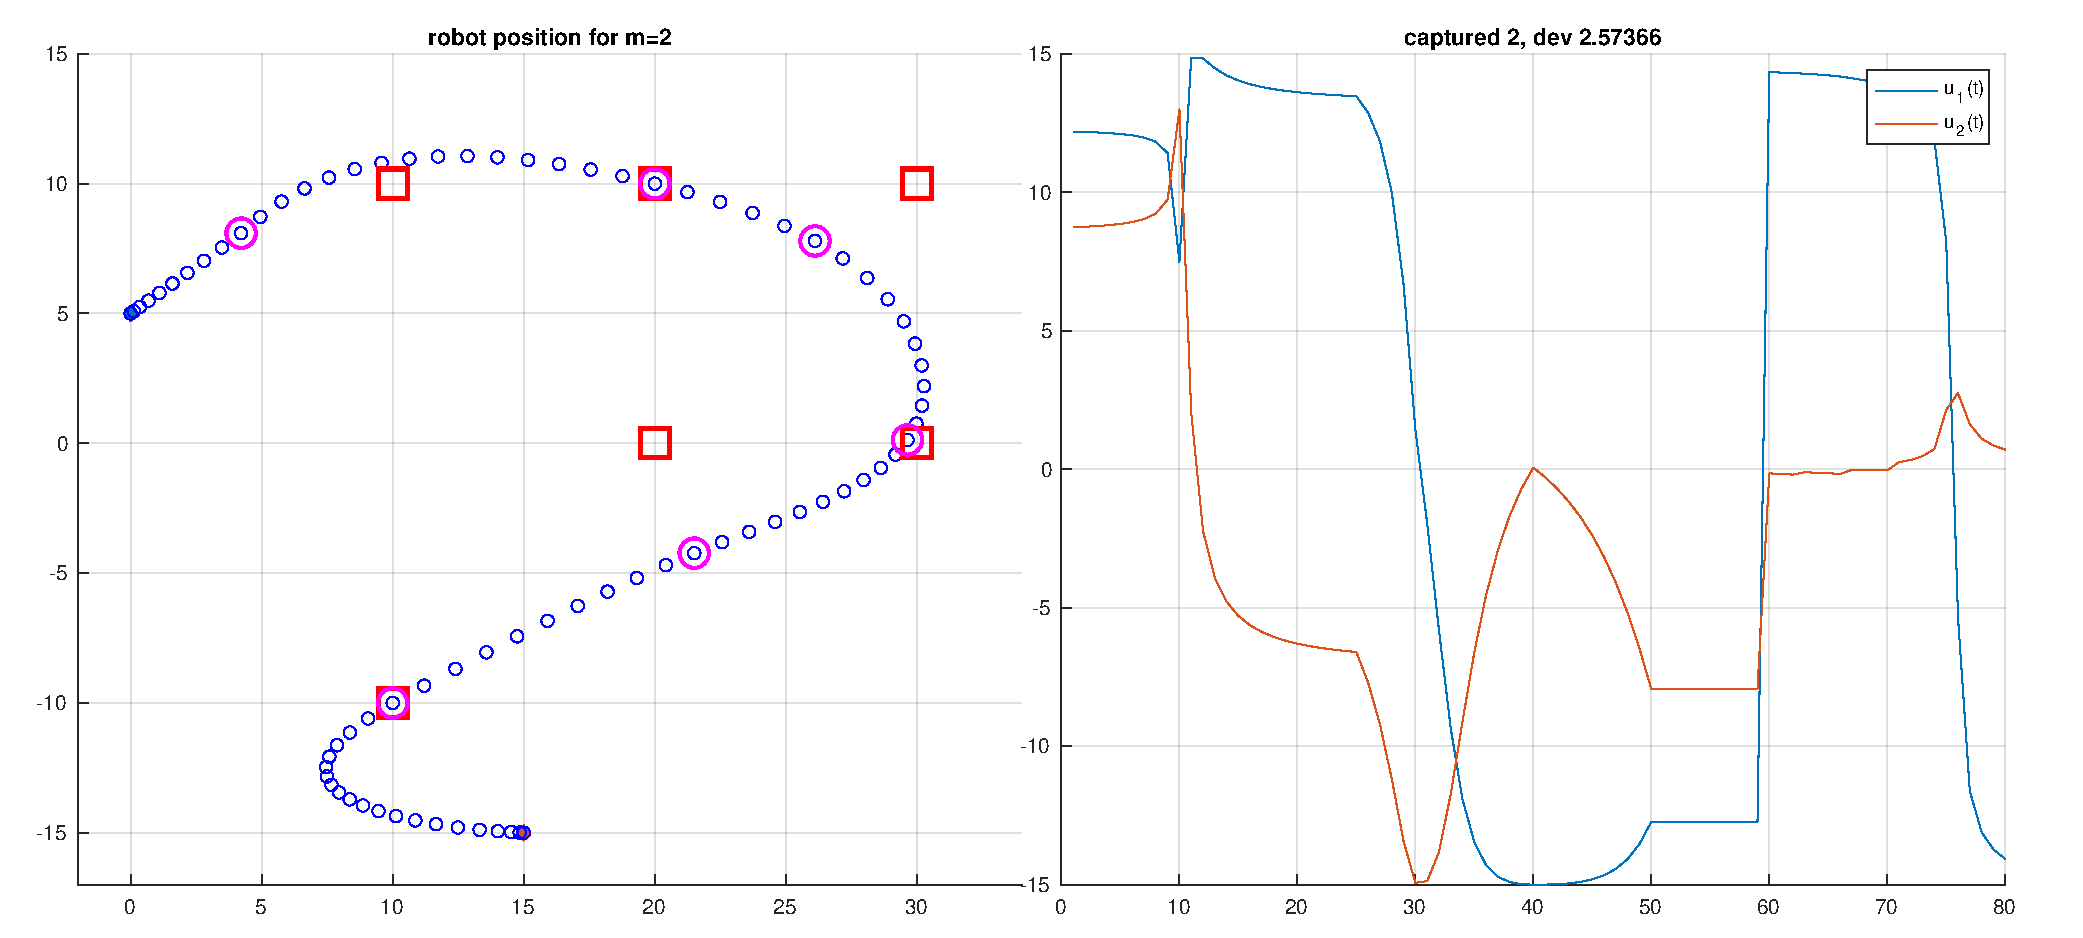
\includegraphics[width=0.5\linewidth]{part1/figures/task11/task_11_2.pdf}\hspace{0em}
        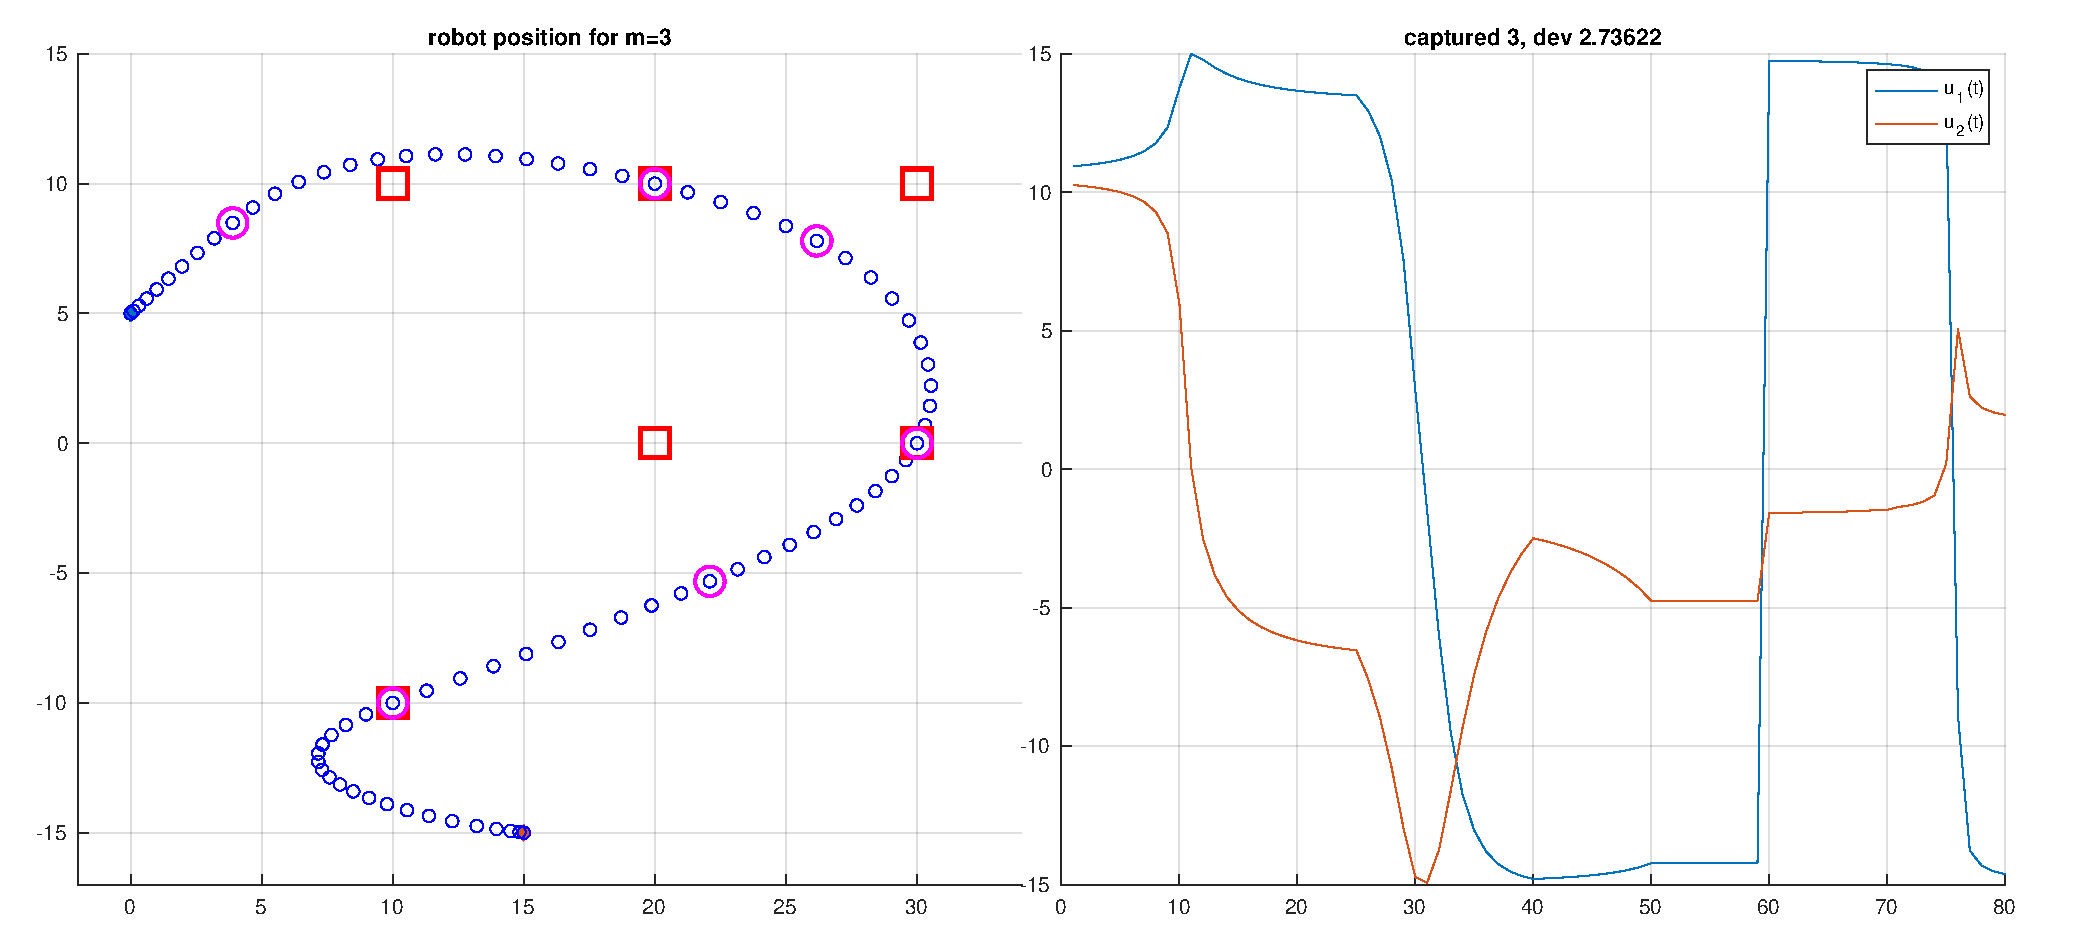
\includegraphics[width=0.5\linewidth]{part1/figures/task11/task_11_3.pdf}
    \end{subfigure}
    \begin{subfigure}
        \centering
        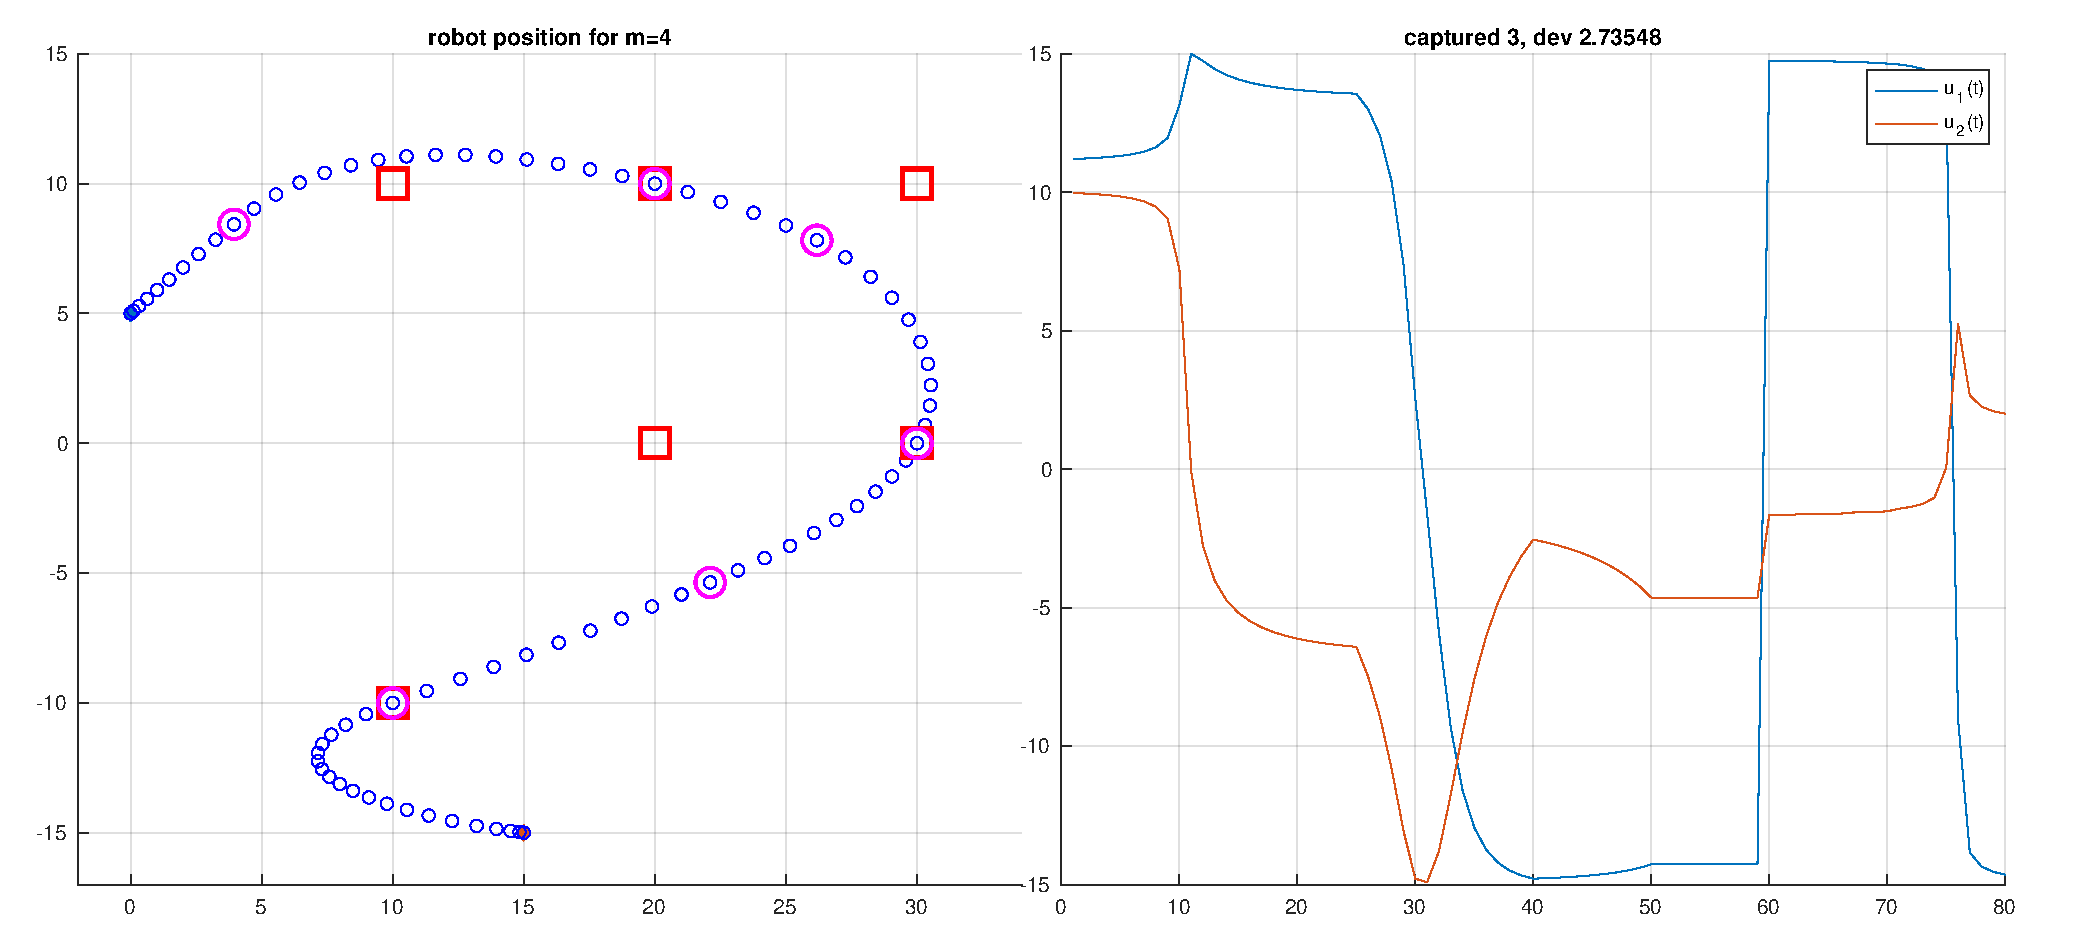
\includegraphics[width=0.5\linewidth]{part1/figures/task11/task_11_4.pdf}\hspace{0em}
        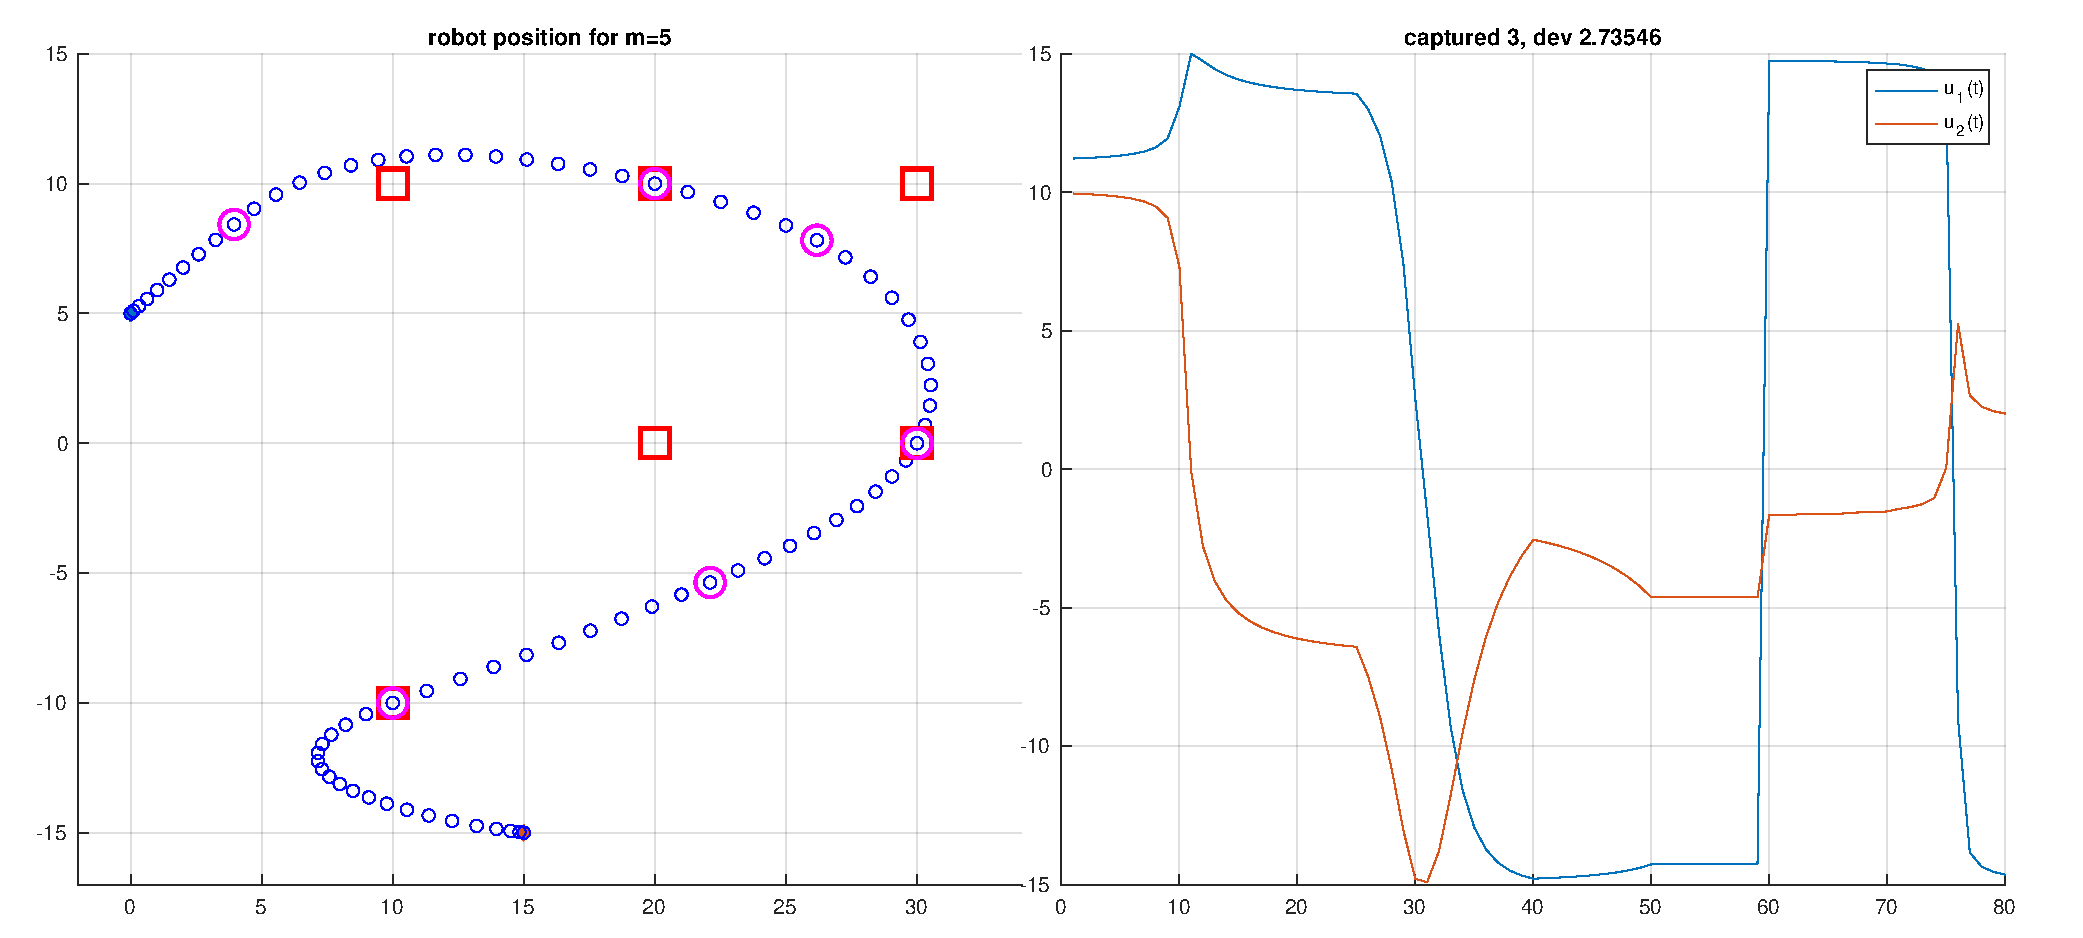
\includegraphics[width=0.5\linewidth]{part1/figures/task11/task_11_5.pdf}
    \end{subfigure}
    \begin{subfigure}
        \centering
        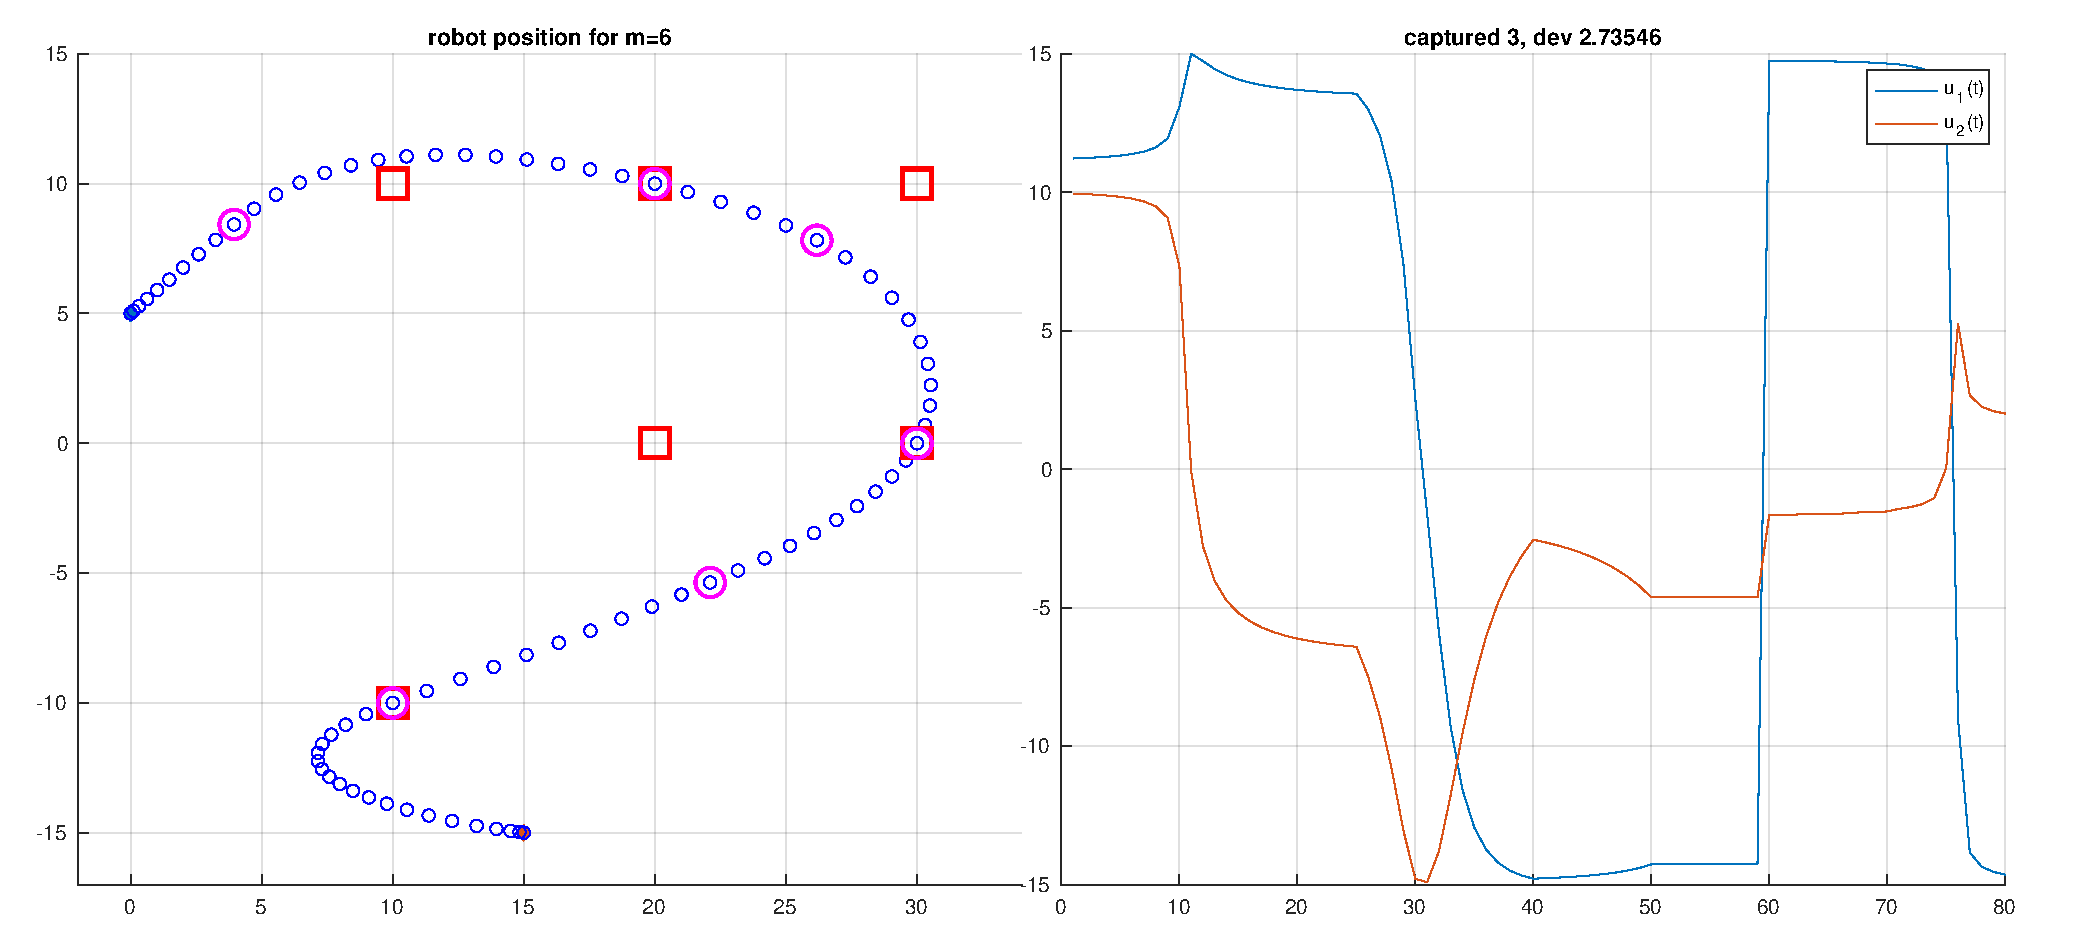
\includegraphics[width=0.5\linewidth]{part1/figures/task11/task_11_6.pdf}\hspace{0em}
        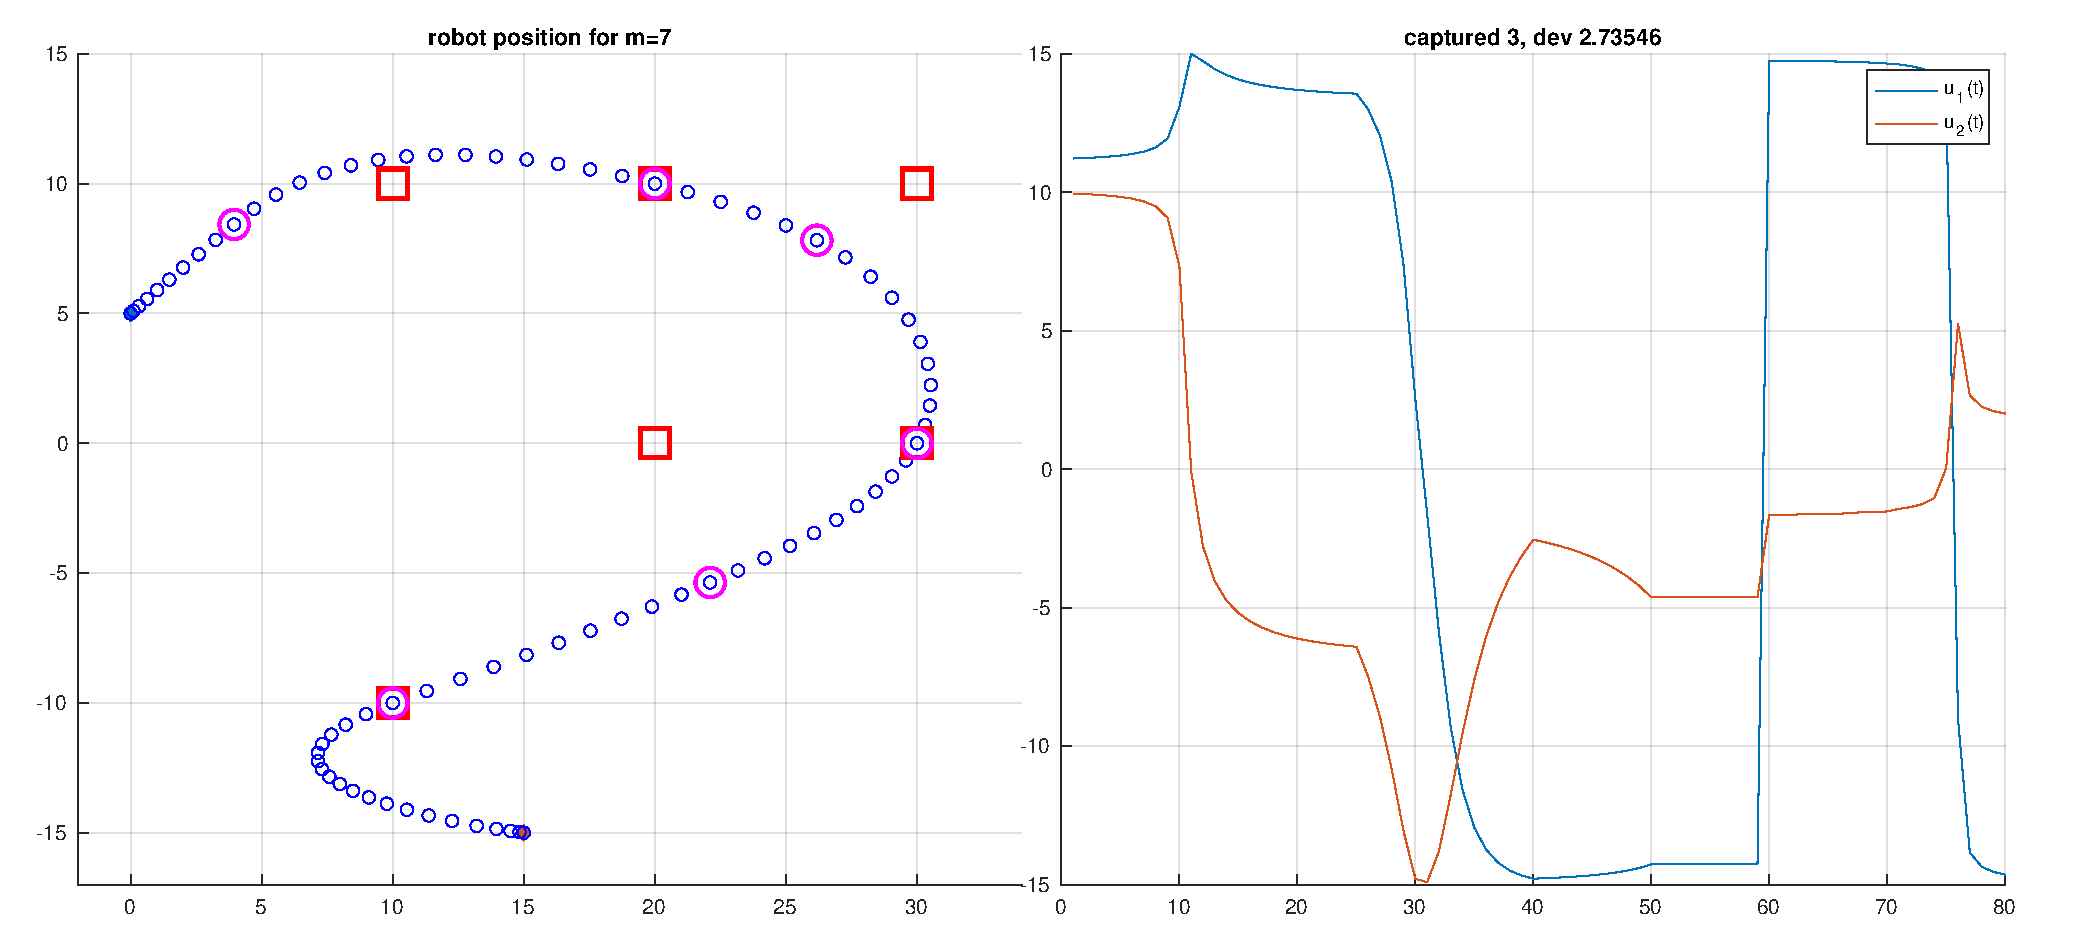
\includegraphics[width=0.5\linewidth]{part1/figures/task11/task_11_7.pdf}
    \end{subfigure}
    \begin{subfigure}
        \centering
        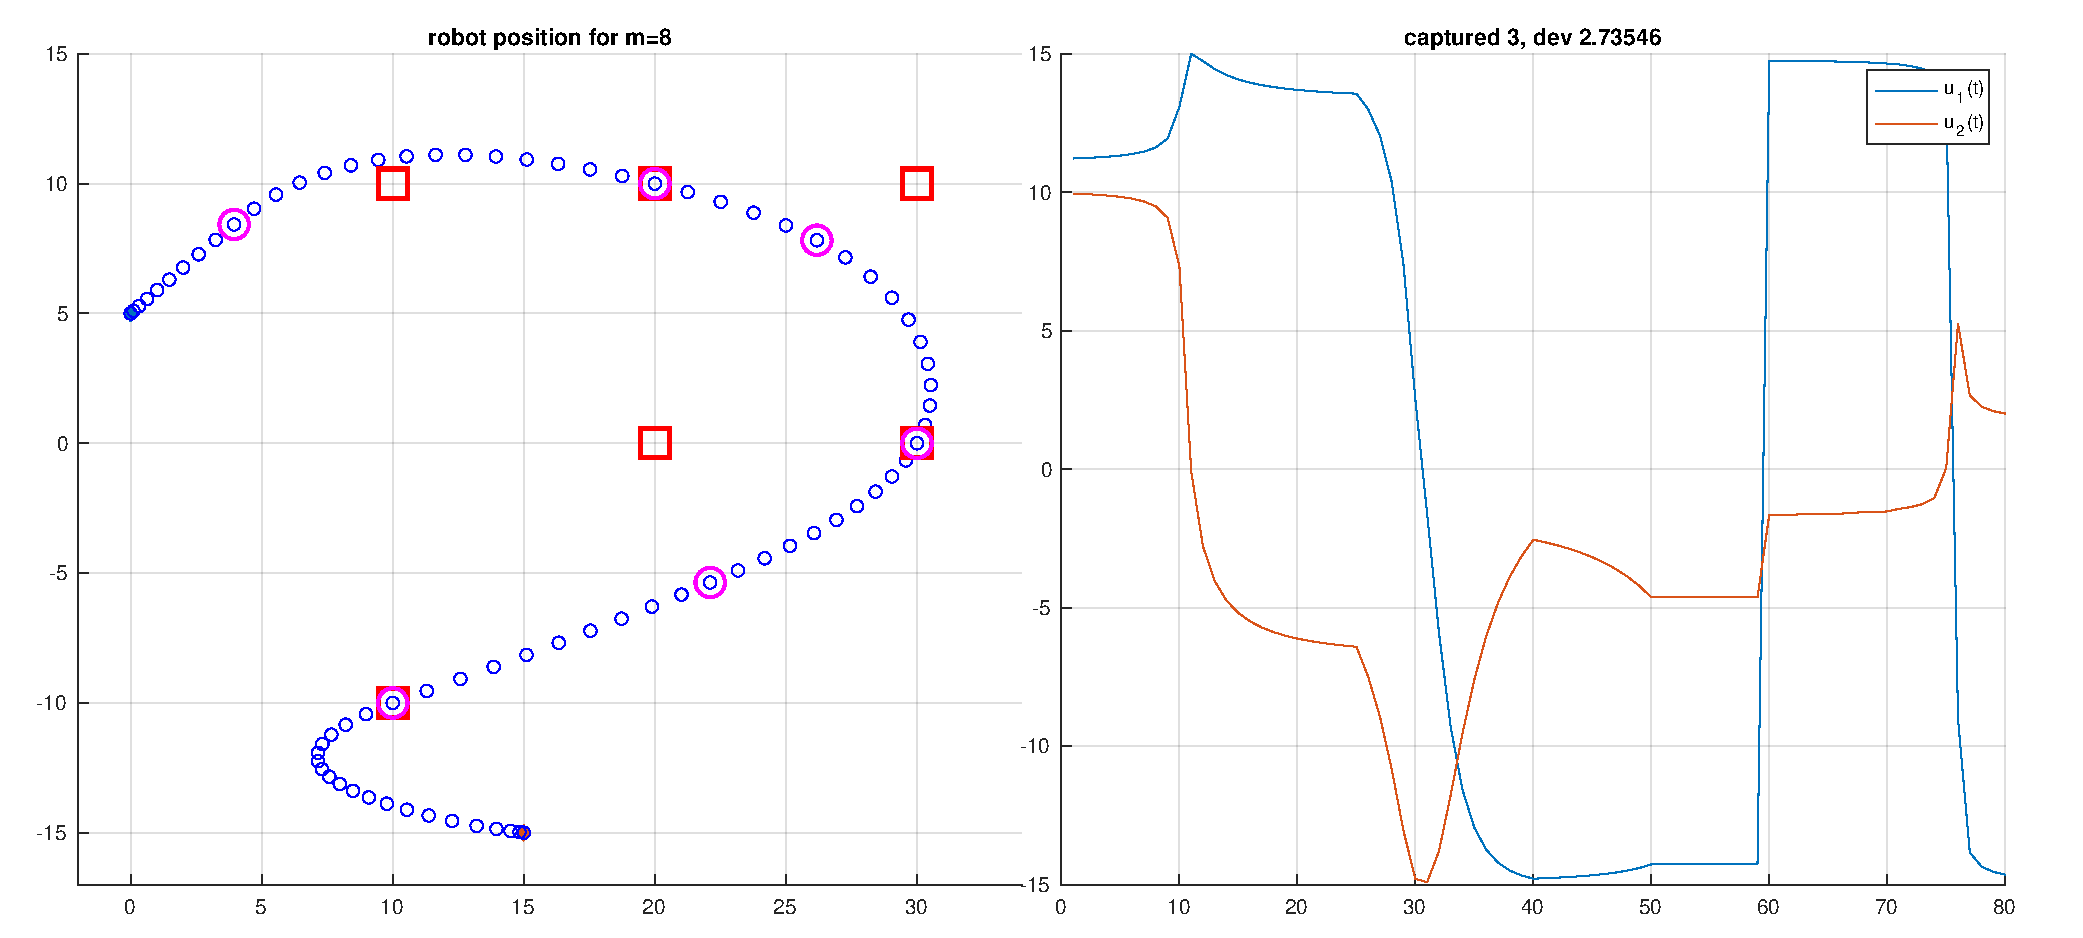
\includegraphics[width=0.5\linewidth]{part1/figures/task11/task_11_8.pdf}\hspace{0em}
        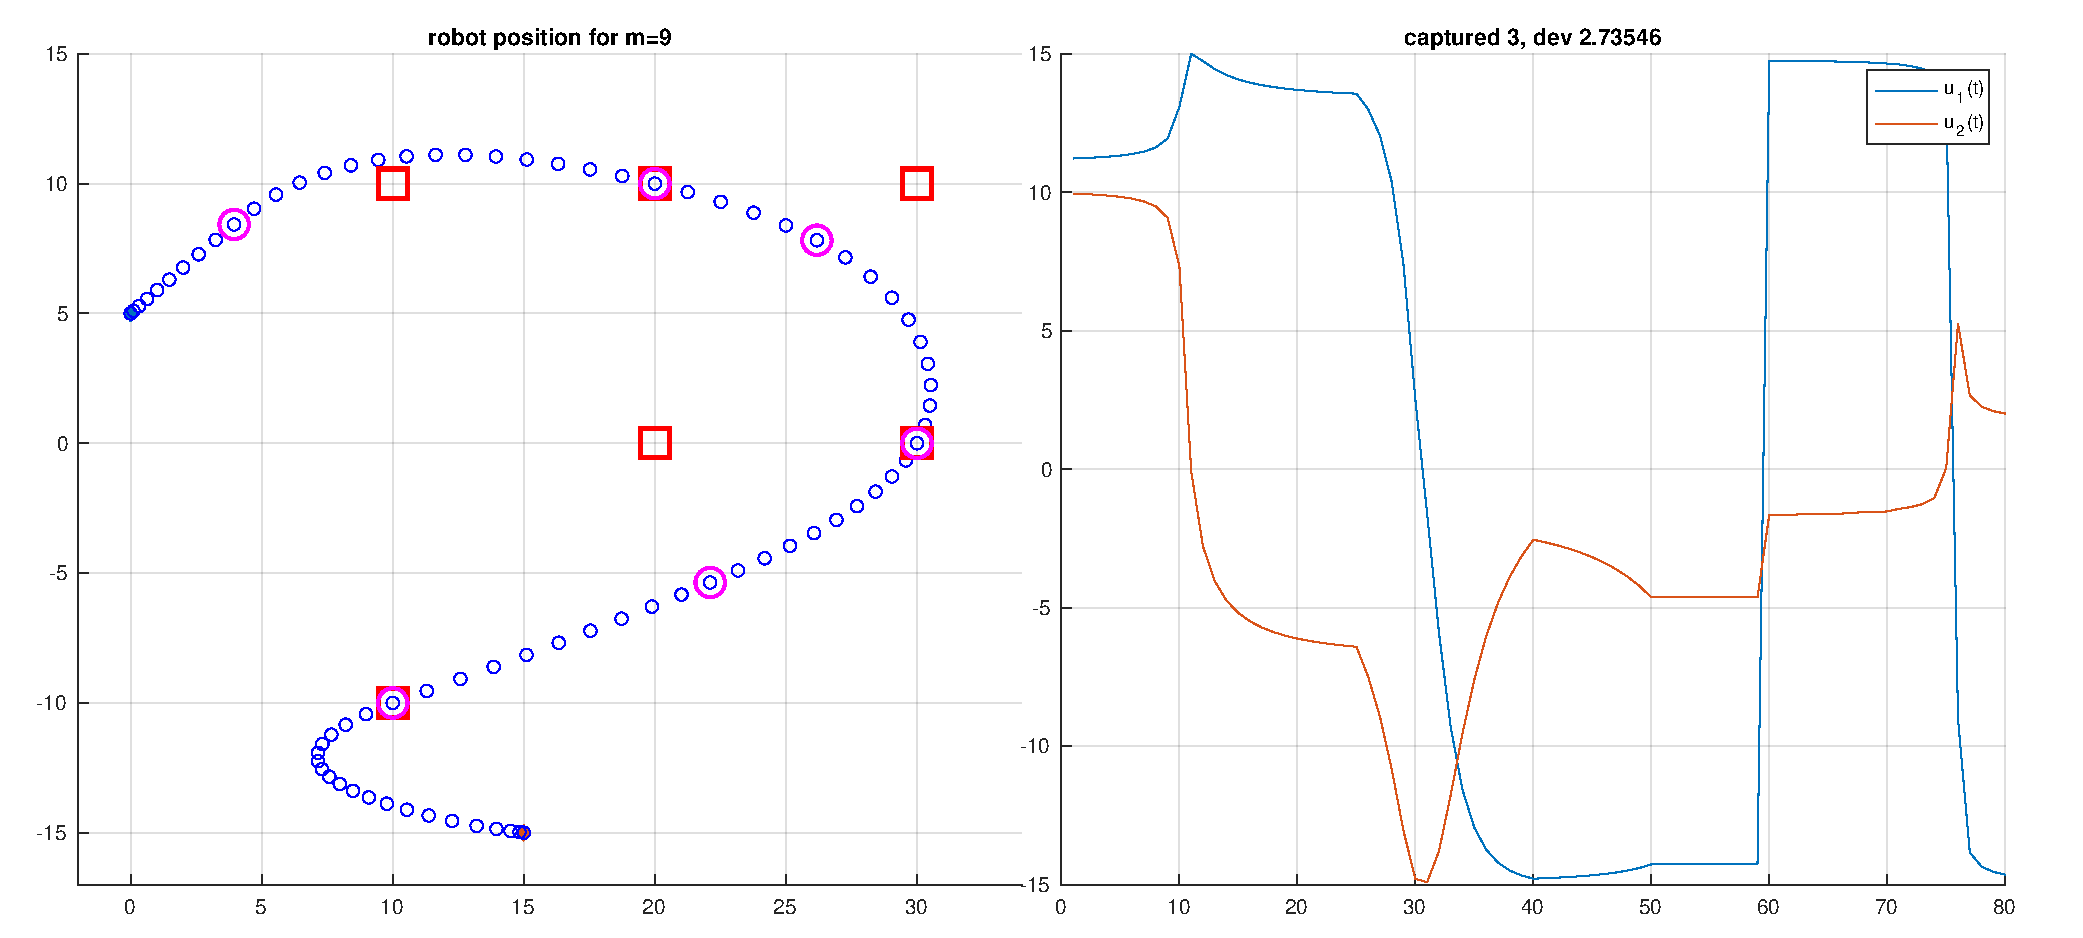
\includegraphics[width=0.5\linewidth]{part1/figures/task11/task_11_9.pdf}
    \end{subfigure}
\end{figure}

\section {Task 12}
%\noindent\fcolorbox{black}{lightgray}{
%    \parbox{\textwidth}{ \textbf{Task 12.} What's the role of the weights in~\eqref{P:prob8}?
%}}

The optimizer tries to optimize the utility function of each waypoint divided by the previous value. The utility values for first 5 iterations are shown in \ref{task12:listing:results}.

\begin{lstlisting}[label=task12:listing:results, caption=Unweighted utility function for each waypoint., float=!htb]
    5.9580    0.9926    3.3379    1.8267    2.3790    0.0000
    6.0346    0.0000    4.3660    1.3281    3.0118         0
    6.0892         0    4.4750    0.3854    4.4923         0
    6.2897         0    4.4125    0.0000    5.7152         0
    6.2540         0    4.3987    0.0000    5.7602         0
    6.2514         0    4.3983    0.0000    5.7630         0
    6.2512         0    4.3983    0.0000    5.7632         0
    6.2512         0    4.3983    0.0000    5.7632         0
    6.2512         0    4.3983    0.0000    5.7632         0
    6.2512         0    4.3983    0.0000    5.7632         0
\end{lstlisting}

By investigating the resulting utility function sizes for each waypoint, we can see that if the robot captures the waypoint, the utlity becomes $0$. Since the optimizer tries to minimize the sum of the utility function for each waypoint, thanks to the reweighting technique, it already has the information from the previous iteration, that the waypoint can be captured. The previous utility value was $0$ and when we divide any number by a very small number ($\epsilon = 10^{-6}$) this fraction explodes thus forcing the optimizer to keep this value small by setting the numerator $0$ again.  